\documentclass{article} % For LaTeX2e
\usepackage{iclr2027_conference,times}
% times.sty silently leaves Latin Modern under some engines; newtxtext pins Times metrics
% so local pagination matches a full TeX Live build. Neither touches the style file.
\IfFileExists{newtxtext.sty}{\usepackage{newtxtext}}{}

% Optional math commands from https://github.com/goodfeli/dlbook_notation.
\input{math_commands.tex}

\usepackage{hyperref}
\usepackage{url}
\usepackage{graphicx}
\usepackage{booktabs}
\usepackage{xcolor}
\usepackage{amsmath,amssymb}
\graphicspath{{figures/}}

\title{When a Blank Is Not a Control: Ablation Choice,\\Generation Budget, and the Attribution\\of Grounding Gains}

% Authors must not appear in the submitted version. They should be hidden
% as long as the \iclrfinalcopy macro remains commented out below.
% Non-anonymous submissions will be rejected without review.

\author{Alexander Mueller \\
Department of Computer Sciences\\
University of Wisconsin--Madison\\
Madison, WI 53706, USA \\
\texttt{amueller.mco@gmail.com} \\
\And
Jae-Ho Lee \\
Visual Intelligence and Graphics Lab \\
Korea University \\
Seoul, South Korea \\
\And
Gyeong-Moon Park \\
Visual Intelligence and Graphics Lab \\
Korea University \\
Seoul, South Korea
}

\newcommand{\rateT}{\ensuremath{H}}
\newcommand{\rateF}{\ensuremath{F}}
\newcommand{\dSight}{\ensuremath{\Delta_{\mathrm{image}}}}
\newcommand{\dBlind}{\ensuremath{\Delta_{\mathrm{ablated}}}}
\newcommand{\dPrim}{\ensuremath{\Delta_{\mathrm{primary}}}}
\newcommand{\civ}[2]{$[#1,\ #2]$}

%\iclrfinalcopy % Uncomment for camera-ready version, but NOT for submission.
\begin{document}

\maketitle

\begin{abstract}
Object-hallucination benchmarks read a better score as better grounding, and the standard check
removes the image to see whether a gain survives. We show that the answer depends on what
replaces the image. We prefill \textsc{LLaVA-1.5-7B}'s description with a passage stitched from
captions of other images, varying only whether they describe one scene or five. A present-minus-absent
score rises by $0.49$, the profile of improved grounding, although only the text changed. With
the image replaced by a grey field the rise is intact, $1.03$ times its sighted size, as our registered
analysis found. In a post-hoc extension to $3{,}500$ images, a mismatched real image, scored where
the sighted generations end before the token budget, leaves $0.47$ of it: about half the rise depends on the image being
the right one. The blank removes the answerable content along with the evidence; on standard benchmarks it
leaves CHAIR with no named objects and POPE with every answer ``no''. With a mismatched image, a published method's POPE gain is image-attributable
($+0.021$ of $+0.022$). A registered yes/no version of our probe does not move, so the effect is
confined to free generation. We recommend reporting both error rates and choosing the ablation
deliberately.
\end{abstract}

\section{Introduction}

When a vision-language model scores better on an object-hallucination benchmark, the improvement is
usually read as better visual grounding. Training-free mitigation methods report better scores as
reduced hallucination \citep{pai, vista, adaiat, regionaware, vcd}, some explicitly as better
grounding \citep{cai, savaa}. Yet the scores also move with caption length and generation budget
\citep{pope, regionaware}, and lower CHAIR can accompany less informative output \citep{safefaith}.
The natural check is to remove the image and ask whether a gain survives: a gain that survives did not
come from looking. This paper shows that the answer to that check depends on what replaces the image.

The check needs the model to keep responding about the scored objects once the image is gone. POPE
\citep{pope} names each candidate object in a question, so its hit rate $H$ on present objects and
false-alarm rate $F$ on absent ones stay measurable whatever the model sees. CHAIR \citep{chair} scores
only the objects the model chooses to mention; its instance score is a false-discovery rate
\citep{throne} whose denominator the model chooses. A fixed candidate list is necessary but not
sufficient: a model that names nothing sets both rates to zero, one that affirms everything sets both
to one, and either corner sends $J = H - F$ to zero. Both occur in published work: blinded
\textsc{LLaVA-1.5} answers ``no'' to everything \citep{lan2026seeing}, sighted \textsc{MultiModal-GPT}
``yes'' \citep{pope}.

\begin{figure}[t]
{\centering
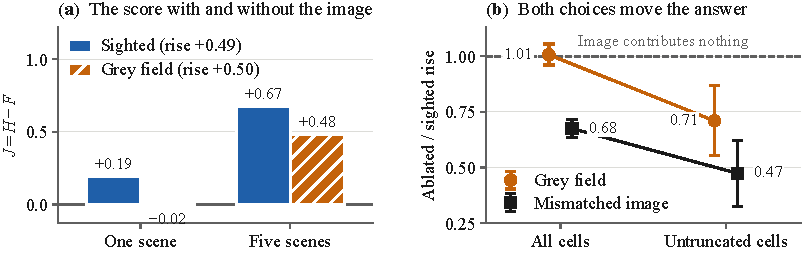
\includegraphics{fig_lead.pdf}\par}
\caption{\textbf{(a)} $J = H - F$ on \textsc{LLaVA-1.5-7B} with the target image and with a uniform grey
field in its place, on the registered $500$ images; every token of text is identical across each pair.
The image raises $J$ by about $0.2$ in each condition and by nearly the same amount in both, so
against \emph{this} ablation the one-to-five-scene rise does not need it. \textbf{(b)} The ablated
rise as a fraction of the sighted one on $3{,}500$ images (post hoc), for two ablations, on all
$10{,}500$ cells and on the $2{,}089$ cells whose sighted continuations both end before the budget;
$95\%$ intervals clustered on the image. A ratio of $1$ means the image contributes nothing.}
\label{fig:lead}
\end{figure}

We build a case in which the cause of a score change is known. We ask \textsc{LLaVA-1.5-7B} to describe
a COCO image and prefill the start of its answer with a short passage cut from human captions of
\emph{other} images, varying only whether those captions describe one other scene or five
(Figure~\ref{fig:example}). The endpoint is how often the continuation repeats an object the passage
names, split by whether the object is in the image ($H$) or not ($F$). Only the text differs between
the conditions, yet the score rises by $0.49$ on its $[-1,1]$ scale ($0.36$ with continuation lengths
matched), mainly because $F$ falls from $0.49$ to $0.11$: the profile a benchmark reader would take as
improved grounding.

Does that rise need the image? Our registered control replaced the image with a uniform grey field,
kept every token of text, and found the rise intact, at $1.03$ times its sighted size
(Figure~\ref{fig:lead}a). A different ablation gives a different answer. In a post-hoc extension to
$3{,}500$ images, a mismatched real photograph in place of the target, scored on cells whose sighted
generations end before the token budget, leaves $0.47$ of the rise, so about half of it depends on the image being the right
one (Figure~\ref{fig:lead}b). The cause of the rise is textual; how much of its effect runs through the
image depends on the control. A grey field removes the image and, with it, the model's ability to
answer about any scene, which hides the part of the rise that needs the correct image.

We contribute three things. (i) A statement of what an image-ablated control must do to attribute a
score change to the image: keep the model responding about the scored objects, and change image
content rather than remove the image, since a blank can also make the ground-truth labels false
(Section~\ref{sec:theory}). (ii) A controlled case in which the standard control's answer is reversed
by the choice of ablation and of generation regime, with the hit and false-alarm rates showing how the
image's contributions cancel inside the score (Section~\ref{sec:results}). (iii) The same analysis on a
published method, PAI \citep{pai}, whose gain passes the content-changing control on CHAIR and POPE
and decomposes mainly into a threshold shift (Section~\ref{sec:mitigation}), with a reporting format
that exposes what a single score hides (Section~\ref{sec:reco}).

\section{What a present-minus-absent score can identify}
\label{sec:theory}

Write $H$ for the rate at which a model names a candidate object that is present in the image and
$F$ for the rate at which it names one that is absent. Scores built on a fixed candidate set are
functions of $(H, F)$; the simplest is $J = H - F$, which has the form of Youden's $J$
\citep{youden1950}. We borrow the correspondence for its decomposition, not to claim that captioning
is a diagnostic test (Appendix~\ref{app:sdt}). CHAIR has a different form. With $P$ present and $A$
absent candidates, counts pooled over captions, and counting mention occurrences as our CHAIR port does
(Appendix~\ref{app:mitig-rates}), $\mathrm{CHAIR}_i = \kappa FA/(HP + \kappa FA)$, where $\kappa$ is
the number of mentions per named absent object divided by the number per named present object. It
falls whenever $\kappa F$ falls proportionally faster than $H$, including when $H$ falls too, so CHAIR
can improve while $J$ worsens.

\paragraph{The score does not isolate sensitivity.} Under an equal-variance Gaussian formulation the
two rates give a separation $d' = Z(H) - Z(F)$ and a threshold $c = -\tfrac{1}{2}[Z(H) + Z(F)]$, with
$Z = \Phi^{-1}$ \citep{snodgrass1988}. Inverting,
\begin{equation}
J \;=\; \Phi\!\left(\tfrac{d'}{2} - c\right) - \Phi\!\left(-\tfrac{d'}{2} - c\right),
\label{eq:J}
\end{equation}
and $\partial J/\partial c = \varphi(-d'/2 - c) - \varphi(d'/2 - c)$ vanishes only where $c\,d' = 0$: for
any non-zero $d'$ the score depends on where the threshold sits. A reader who sees $J$ move cannot tell
whether $d'$ moved, $c$ moved, or both, and, since $J$ is a difference, cannot tell whether an unchanged
$J$ hides opposite movements in $H$ and $F$. Nor does $d'$ settle the question. It measures how well
behaviour separates the two populations using whatever information the model has, and the text in the
prompt, including which objects it puts up for scoring, is part of that information. Nothing in
Equation~\ref{eq:J} distinguishes separability achieved by looking at the image from separability
achieved through the text.

\paragraph{Which counterfactual attribution needs.} Let $\Delta(x)$ be the change in $J$ that an
intervention produces with image $x$. Its image-attributable part is defined against a counterfactual
input $\tilde{x}$ that replaces the image: $\dSight = \Delta(x) - \Delta(\tilde{x})$. Two choices of
$\tilde{x}$ answer different questions. A blank asks whether the change needs \emph{an} image; another
image from the same distribution asks whether it needs \emph{this} image. A claim of better grounding
is of the second kind, since it says the output now tracks what the image shows, and the two coincide
only if removing the image leaves the model's behaviour on the scored objects otherwise intact. A blank
can fail that in two ways: it can leave nothing to score, and it can move the model to an operating
point where it no longer answers about any scene, so that the image effect it removes is not the one
the intervention acts on. A mismatched image keeps the model answering about a real scene, the
counterfactual that measures of cross-modal interaction use \citep{hessel2020emap, gat2021perceptual};
its cost is that the substitute can contain some of the scored objects, which biases $\dSight$ towards
zero (Section~\ref{sec:twofactors}).

\section{Method}
\label{sec:method}

\begin{figure}[t]
\centering\footnotesize
\setlength{\tabcolsep}{4pt}
\renewcommand{\arraystretch}{1.12}
\begin{tabular}{@{}p{0.115\textwidth}p{0.855\textwidth}@{}}
\toprule
\multicolumn{2}{@{}l}{Image 146155 (COCO). Annotated objects: bottle, \textbf{person}, wine glass.} \\
\midrule
\textbf{One scene} & \emph{Passage:} A \underline{dog} and its owner playing \underline{Frisbee}, in the dirt. A \textbf{man} and two \underline{dogs} playing with an object. A \textbf{man} and two \underline{dogs} on \\
Sighted & a beach. A \textbf{man} and two \underline{dogs} playing with an object. {\color{gray}[repeated to the budget]} \\
Grey field & a field. A \underline{dog} and its owner playing \underline{Frisbee}. A \underline{dog} and its owner playing \underline{Frisbee} in the dirt. \\
Mismatched & a field. A \textbf{woman} and a \underline{dog} playing with a \underline{frisbee}. {\color{gray}[repeated to the budget]} \\
\midrule
\textbf{Five scenes} & \emph{Passage:} \textbf{People} with \underline{ski} and \underline{snowboard} equipment shaking hands. A little \textbf{boy} wearing a baseball hat holding a \underline{baseball bat}. A \textbf{person} stands between two \underline{dogs} on a \\
Sighted & leash. A \textbf{man} and a \textbf{woman} standing in front of a wine rack. {\color{gray}[repeated to the budget]} \\
Grey field & leash. A \textbf{person} with a backpack on their back. {\color{gray}[repeated to the budget]} \\
Mismatched & leash. A \textbf{woman} wearing sunglasses and a green shirt. A \textbf{man} wearing a white shirt. {\color{gray}[\ldots]} \\
\bottomrule
\end{tabular}
\caption{One cell of the stimulus, chosen for legibility, with the continuation of each arm. Objects
the passage names are scored: \textbf{bold} if annotated in the image, \underline{underlined} if not.
With one scene every arm repeats absent objects; with five, every arm names only the present one, with
or without the correct image. The sighted arm alone mentions the wine rack it sees.}
\label{fig:example}
\end{figure}

\paragraph{Stimulus.} We ask the model to describe the image and prefill the start of its answer with a
passage built from five human COCO captions of other images: in the one-scene condition all five
describe one other image, in the five-scene condition five different images. They are shuffled, joined
and cut to a per-cell token length --- on \textsc{LLaVA-1.5-7B} the smaller of half the model's own
caption length and the length of a natural-prose description of the first source image, $44.6$ tokens
on average (Appendix~\ref{app:setup}) --- so a passage can end mid-word, and the model continues
greedily up to a budget of $384$ tokens. A \emph{cell} is one image with its passage draw in both
conditions, and each image contributes three. Both conditions have the same passage length; after the
cut the five-scene passage covers about $2.7$ distinct scenes against $1.0$ and twice as many object
types. A continuation that reaches the budget is \emph{truncated}: $45\%$ of one-scene and $68\%$ of
five-scene continuations are, many repeating one sentence (Figure~\ref{fig:example}).

\paragraph{Endpoint.} A \emph{unit} is an (image, object type named in the passage) pair, and the model
carries a unit forward if its continuation names that object type. $H$ and $F$ are carry-forward rates
over units whose object is and is not in the image's COCO annotations, and $\dPrim$ is the change in
$J$ from one scene to five. This endpoint was adopted after CHAIR proved unusable on these conditions
(Appendix~\ref{app:prereg}).

\paragraph{Ablations.} Each ablated arm reruns the pipeline with the target image replaced and every
token of text unchanged, so it scores the same units with the same labels. The \emph{grey field} is a
flat mid-grey image of the target's size. The \emph{mismatched image} is another image of the same
sample, assigned by a derangement: a random permutation of the images that maps none to itself. With
$\dBlind$ the contrast in the ablated arm, the image-attributable part is $\dSight = \dPrim - \dBlind$,
and $\dBlind/\dPrim$ is the share of the rise that survives the ablation. We call each image condition --- sighted, grey
field, mismatched image --- an \emph{arm}.

\paragraph{Samples, registration and inference.} The registered sample is $500$ COCO val2017 images
($1{,}500$ cells), and the extension is $3{,}500$ images that contain them ($10{,}500$ cells). We call
an analysis registered when a written plan with its decision rules was committed to our git
repository before the corresponding generation job; the timestamps are our own, not a third-party
registry's, and Appendix~\ref{app:prereg} lists each registration with its commit hash. Seeds encode
the date an analysis was fixed (the derangement's is $20260919$), so they also record the timeline. The
grey-field analyses and the mismatched image on the registered sample are registered, the latter by a
dated amendment written before its data existed; the $3{,}500$-image comparison of the two ablations
is post hoc. Intervals are $95\%$ paired bootstraps clustered on the image, $B = 4000$.

\section{Results}
\label{sec:results}

\subsection{A large rise with a textual cause}
\label{sec:exp1}

On \textsc{LLaVA-1.5-7B} the score rises from $+0.19$ to $+0.67$, a contrast of $+0.49$
\civ{+0.43}{+0.54}. It is the least controlled number we report: matching continuation lengths leaves
$+0.36$ \civ{+0.30}{+0.41}, and restricting to untruncated cells of the $3{,}500$-image sample leaves
$+0.35$ \civ{+0.28}{+0.41} (Appendix~\ref{app:regime}). Units whose object is in the image are enriched
for frequent objects the model names anyway, a non-visual route to a higher score: stratifying by
object frequency leaves $+0.33$ \civ{+0.22}{+0.44}, and because every arm scores the same units, this
composition effect cancels from $\dSight$ to first order (Appendix~\ref{app:robust}). With lengths
matched, $H$ barely moves ($-0.03$ \civ{-0.08}{+0.02}) while $F$ falls from $0.46$ to $0.08$. The rise
is monotone over a five-point grid in the number of scenes and replicates on
\textsc{LLaVA-OneVision-0.5B} ($+0.38$ \civ{+0.32}{+0.43}; Appendix~\ref{app:models}).

\paragraph{The rise is specific to assembled captions and to free generation.} A registered version
that builds the passage from natural prose (Localized Narratives) instead of COCO captions was null
($+0.01$ \civ{-0.04}{+0.05}), under every specification, though it realised about half the headline's
dose; by that registration, the lead result is specific to the assembled-caption construct. An earlier
registered natural-prose run did score five sources above one, by $+0.07$ \civ{+0.02}{+0.13} raw but
only $+0.02$ \civ{-0.03}{+0.07} length-matched. A registered yes/no version of the probe on the same
units does not move ($-0.01$ \civ{-0.03}{+0.01}), and by that registration every claim here concerns
free generation (Appendix~\ref{sec:forced}).

\subsection{The registered control: a grey field}
\label{sec:blind}

\begin{table}[t]
\caption{The one-scene to five-scene contrast with the image and under the grey field, on truncated
generations as registered. $\dSight = \dPrim - \dBlind$; bold marks intervals that exclude zero. The
last column is the share of the rise that survives the grey field. \textsc{Qwen3-VL-8B} is documented in
Appendix~\ref{app:qwen3}; \textsc{Qwen2.5-VL-7B}, which is not interpreted, is in
Appendix~\ref{app:models}.}
\label{tab:models}
\begin{center}
\small
\begin{tabular}{lrrlr}
\toprule
Architecture & Sighted $\dPrim$ & Grey $\dBlind$ & $\dSight$ & Grey/sighted \\
\midrule
\textsc{LLaVA-1.5-7B}          & $+0.486$ & $+0.502$ & $-0.016$ \civ{-0.070}{+0.040} & $1.03$ \\
\textsc{LLaVA-OV-0.5B}         & $+0.378$ & $+0.413$ & $-0.035$ \civ{-0.091}{+0.018} & $1.09$ \\
\textsc{Kosmos-2}              & $+0.215$ & $+0.318$ & $\mathbf{-0.103}$ \civ{-0.168}{-0.036} & $1.48$ \\
\textsc{Qwen3-VL-8B}           & $+0.583$ & $+0.523$ & $\mathbf{+0.060}$ \civ{+0.024}{+0.096} & $0.90$ \\
\bottomrule
\end{tabular}
\end{center}
\end{table}

Table~\ref{tab:models} gives the contrast with the image and under the grey field on four
architectures. On \textsc{LLaVA-1.5-7B} the grey rise is $1.03$ \civ{0.92}{1.16} times the sighted
one. \textsc{LLaVA-OV-0.5B} agrees, although its grey continuations are short (medians of five and
eleven tokens against $192$ sighted). The other two depart in opposite directions: on \textsc{Kosmos-2}
the rise is larger without the image, and on \textsc{Qwen3-VL-8B} about a tenth of it needs the image,
though its arms repeat sentences at different rates (Appendix~\ref{app:qwen3}). \textsc{Qwen2.5-VL-7B}
produced four- or five-token continuations in every arm and is not interpreted, as its registration
committed in advance (Appendix~\ref{app:models}).

The grey null is not a failure to use the image. Within each condition the image raises $J$ by
$+0.21$ \civ{+0.16}{+0.26} and $+0.19$ \civ{+0.16}{+0.23} on \textsc{LLaVA-1.5-7B}, and raises $d'$ in
every condition (Appendix~\ref{app:dprime-table}); because that effect is nearly equal in the two
conditions, it cancels from $\dSight$. It is not equal in $H$ and $F$ separately
(Table~\ref{tab:report}): under grey the image contributes $-0.14$ to the rise in $H$ and $-0.12$ to
the rise in $F$, and the two cancel in $J$. The grey null holds under three ground-truth constructions,
every registered truncation rule and a length match; the registered mention-rate control fails on five
of sixteen powered subsets, four of them with $\dSight$ near $+0.10$ (Appendix~\ref{app:robust}).

\subsection{The ablation and the generation regime}
\label{sec:twofactors}

\paragraph{Two choices, each sufficient to move the answer.} Both factors were run on all $10{,}500$
cells of the $3{,}500$-image sample, with identical passages: the grey field and the mismatched image,
each scored on all cells and on the $2{,}089$ untruncated cells, those in which neither sighted
continuation reaches the budget (Appendix~\ref{app:regimeblind}). On all cells the grey field
reproduces the registered null (ratio $1.01$ \civ{0.96}{1.05}) and the mismatched image the
registered sample's $0.67$ ($0.68$ \civ{0.64}{0.72}). On untruncated cells the ratios fall to $0.71$
\civ{0.56}{0.87} and $0.47$ \civ{0.33}{0.62} (Figure~\ref{fig:lead}b). Each factor moves the answer at
either level of the other, and together they take the image's share of the same rise from nothing to
about half, $\dSight = +0.18$ \civ{+0.12}{+0.24}. The substitute image also contains $46$--$48\%$ of
the present objects the passage names ($10$--$12\%$ of the absent ones); excluding those units raises
$\dSight$ on all cells from $+0.15$ to $+0.24$ \civ{+0.21}{+0.27}, so the substitution estimates are
conservative. On \textsc{Qwen3-VL-8B} only the ablation factor can be run, since $94\%$ of its
continuations reach the budget and $14$ cells are untruncated. There the two ablations agree: $\dSight$
is $+0.065$ \civ{+0.031}{+0.100} with a mismatched image and $+0.060$ with grey (ratios $0.89$ and
$0.90$). That model's sighted one-scene $J$ is already near zero ($+0.05$), so grey has no level to
remove, which fits the mechanism below, though we read it post hoc (Appendix~\ref{app:qwen3}).

\paragraph{Why the grey field hides the contribution.} $\dSight$ is the difference between the image's
effect on $J$ in the five-scene and the one-scene condition, and grey removes both. With one scene it
drops $H$ from $0.68$ to $0.47$, level with $F$ ($0.49$), so $J$ starts at zero; with five it lowers
$J$ by a similar amount, and the two removals cancel. The mismatched image leaves the model a scene
to answer about: its one-scene $H$ stays at $0.64$, and what it removes is the five-scene rise in $H$
that needs the correct image, since $H$ falls from $0.64$ to $0.60$ where the sighted arm's rises from
$0.68$ to $0.78$. Table~\ref{tab:report} shows the contribution sits in $H$, not $F$.

\paragraph{Which ablations blind the model.} Of the ten ablations run on the registered sample
(Appendix~\ref{app:ladder}), five barely remove the image: under pixel noise, light blur and patch
shuffling the one-scene $J$ stays between $+0.14$ and $+0.18$, against $+0.19$ sighted, so their null
$\dSight$ says little. The four that do remove it --- grey, black, heavy blur and $16{\times}16$
downsampling --- collapse the one-scene $J$ to between $-0.02$ and $+0.03$, and all four return
$\dSight$ near zero. Only the substitution removes the correct image while leaving an answerable one,
and only it returns a positive $\dSight$ ($+0.16$ \civ{+0.11}{+0.21}), which survives matching
continuation lengths across conditions ($+0.14$ \civ{+0.10}{+0.18}).

\begin{table}[t]
\caption{The rise on \textsc{LLaVA-1.5-7B} (registered sample), decomposed under each ablation. The
first three columns are one-to-five-scene changes; the last two are the image-attributable parts,
sighted minus ablated, with $95\%$ intervals. Columns round independently. $^{*}$Post hoc for this
contrast. This is the reporting format we recommend (Section~\ref{sec:reco}).}
\label{tab:report}
\begin{center}
\small
\setlength{\tabcolsep}{4.5pt}
\begin{tabular}{lrrrll}
\toprule
& \multicolumn{3}{c}{Change, one to five scenes} & \multicolumn{2}{c}{Image-attributable} \\
\cmidrule(lr){2-4}\cmidrule(l){5-6}
Quantity & Sighted & Grey & Mismatched & Grey field & Mismatched image \\
\midrule
Hit rate $H$             & $+0.10$ & $+0.24$ & $-0.05$ & $-0.14$ \civ{-0.19}{-0.08} & $+0.15$ \civ{+0.10}{+0.20} \\
False-alarm rate $F$     & $-0.38$ & $-0.26$ & $-0.37$ & $-0.12$ \civ{-0.15}{-0.10} & $-0.01$ \civ{-0.03}{+0.01} \\
Score $J$                & $+0.49$ & $+0.50$ & $+0.33$ & $-0.02$ \civ{-0.07}{+0.04} & $+0.16$ \civ{+0.11}{+0.21} \\
Separation $d'^{*}$      & $+1.53$ & $+1.35$ & $+0.97$ & $+0.19$ \civ{+0.03}{+0.35} & $+0.56$ \civ{+0.40}{+0.72} \\
Threshold $c^{*}$        & $+0.45$ & $+0.04$ & $+0.61$ & $+0.41$ \civ{+0.32}{+0.50} & $-0.16$ \civ{-0.24}{-0.07} \\
\bottomrule
\end{tabular}
\end{center}
\end{table}

\paragraph{Decomposition.}\label{sec:decomp} Under either ablation the image changes the rates, but differently
(Table~\ref{tab:report}). Against grey it lowers the rise in $H$ and deepens the fall in $F$ by
similar amounts, which cancel in $J$; against the mismatched image it adds to the rise in $H$ and
leaves $F$ alone. In signal-detection terms the correct image contributes separation ($d'$ $+0.56$
\civ{+0.40}{+0.72}) against the mismatched image, but mostly threshold ($c$ $+0.41$) against grey,
because the grey field moves the threshold itself. Separation still rises in every arm ($d'$ gains
$1.53$ sighted, $1.35$ under grey and $0.97$ with the mismatched image), so on this construction
much of it comes from the text. These
coordinates recode the two rates exactly but were not registered for this contrast, and we do not
claim the equal-variance model holds: one operating point cannot test it, and mixtures can mimic
unequal variance \citep{decarlo2002}. The argument needs only Equation~\ref{eq:J} and the rates.

\section{A published method on CHAIR and POPE}
\label{sec:mitigation}

We applied the same decomposition to PAI \citep{pai}, a training-free method that amplifies attention
to image tokens during decoding, on \textsc{LLaVA-1.5-7B} captioning $500$ COCO images at its
prescribed strength. This analysis was registered in advance (Appendix~\ref{app:mitig}); the scored
units are all $80$ COCO categories per image, so $H$ and $F$ are defined, and because $F$ is about
$0.01$, $J$ is essentially $H$. At the repository's default strength the method has no CHAIR gain to
decompose ($\Delta\mathrm{CHAIR}_i$ $-0.26$ \civ{-1.42}{+0.91}), so everything below is at the
prescribed setting.

\begin{table}[t]
\caption{PAI against the unmodified model on standard CHAIR (\textsc{LLaVA-1.5-7B}, $500$ COCO
images). Lower $\mathrm{CHAIR}_i$ is better. The change row gives PAI minus vanilla, with $95\%$
intervals beneath; here $d'$ and $c$ were registered in advance.}
\label{tab:pai}
\begin{center}
\small
\setlength{\tabcolsep}{3.4pt}
\begin{tabular}{lrrrrrr}
\toprule
Arm & $\mathrm{CHAIR}_i$ & $H$ & $F$ & $J$ & $d'$ & $c$ \\
\midrule
Vanilla              & $12.8$ & $0.78$ & $0.010$ & $0.77$ & $3.10$ & $0.77$ \\
PAI ($\alpha = 0.5$) & $7.2$  & $0.71$ & $0.005$ & $0.70$ & $3.12$ & $1.01$ \\
\midrule
Change & $-5.6$ & $-0.07$ & $-0.005$ & $-0.07$ & $+0.02$ & $+0.24$ \\
       & \scriptsize[$-7.1$,\,$-3.9$] & \scriptsize[$-0.09$,\,$-0.05$] & \scriptsize[$-0.006$,\,$-0.004$] & \scriptsize[$-0.09$,\,$-0.05$] & \scriptsize[$-0.06$,\,$+0.09$] & \scriptsize[$+0.20$,\,$+0.28$] \\
\bottomrule
\end{tabular}
\end{center}
\end{table}

PAI lowers $\mathrm{CHAIR}_i$ from $12.8$ to $7.2$ (Table~\ref{tab:pai}). That PAI buys precision with
recall is already established: \citet{sparc} report precision rising from $84.70$ to $90.64$ and recall
falling from $79.46$ to $72.44$ for PAI on \textsc{LLaVA-1.5} over $500$ COCO images. Our $H$ is that
recall, and it falls by $0.07$ against their $0.0702$, a check on the recoding rather than a finding.
What the decomposition adds is that the rate of naming absent objects also halves, so CHAIR improves
while $J$ worsens by $0.07$, the two summaries ordering the same captions oppositely. Probit $d'$ does
not move and the threshold does: moving $c$ alone accounts for a change in $J$ of $-0.07$, moving $d'$
alone for $+0.003$ (Appendix~\ref{app:zroc}). Shortening the unmodified model's own captions until
its $F$ matches PAI's gives $\mathrm{CHAIR}_i$ of $8.0$ \civ{6.9}{9.3}, a difference from PAI of $-0.8$
\civ{-1.8}{+0.4}; truncation is a standard length baseline \citep{lessismore}, but shortening is not a
pure threshold change, so this places PAI near the unmodified model's trajectory rather than on it.
Whether a small separation gain accompanies the shift the registered test could not decide: a log-odds
measure rises ($+0.30$ \civ{+0.13}{+0.48}) while probit $d'$ and the matched-$F$ comparison do not.

\paragraph{The ablation control on CHAIR.} No uniform field can run it: under grey, and equally under
black, the model names none of the $80$ categories in any of $500$ captions, with or without PAI, so
$\mathrm{CHAIR}_i$ is $0/0$. A mismatched image keeps the model naming objects. PAI's $\mathrm{CHAIR}_i$
gain then falls to $+0.4$ \civ{-1.2}{+2.0}, leaving $+5.2$ \civ{+2.9}{+7.4} attributable to the image,
which the ablation study's registered rule classifies as image-attributable (Appendix~\ref{app:ladder}).

\paragraph{The ablation control on POPE.} On official POPE with a mismatched image, PAI's
attention-only configuration --- which reproduces its published gain, $+1.10$ accuracy points against
their $+1.06$ --- raises $J$ by $+0.022$ \civ{+0.011}{+0.034} sighted and $+0.001$ \civ{-0.010}{+0.012}
ablated, so $\dSight = +0.021$ \civ{+0.004}{+0.037}. The gain needs the image; the registered rule
certifies it only as partly image-attributable because the lower bound falls just below half the gain.
Under a grey field the same test cannot run: the model answers ``no'' to all $9{,}000$ questions,
correctly, since a grey field contains none of the queried objects, so $H = F = 0$ by construction
(Appendix~\ref{app:pope}). The released \texttt{--use-attn --use-cfg} configuration shows no gain at
all, because it suppresses the amplification at the prefill position that carries a one-token answer.
PAI's own published POPE table decomposes the same way: on balanced splits $F = H + 1 - 2\,\mathrm{acc}$
and $H$ follows from accuracy and F1, giving $\Delta d' = +0.04$ against $\Delta c = +0.18$
(Appendix~\ref{app:pope}).

On both benchmarks, then, PAI's gain is tied to the image and is mainly a threshold shift, whose
separation component the registered test could not resolve. Nothing here says the improvement is
spurious, only that $\mathrm{CHAIR}_i$ alone cannot say which kind of improvement it is, and that the
rates which can are already computed wherever CHAIR is.

\section{Recommended reporting}
\label{sec:reco}

\begin{enumerate}
\itemsep0.1em
\item \textbf{Report $H$ and $F$ with their decomposition, not a single score.} Report the
image-attributable part of each rate, since a null on $J$ can hide offsetting effects on the two, and
$d'$ and $c$ where the question is separation against threshold (Table~\ref{tab:report}). For CHAIR,
report the $H$ and $F$ its mention records already contain (Table~\ref{tab:pai}).
\item \textbf{Ablate every endpoint whose candidates the input supplies, and choose the ablation for
the question.} A question naming each object, as in POPE, or a passage naming it, as here, keeps the
model answering about every scored object without the image. To test grounding, change the image's
content rather than remove it, and report the ablated arm's levels in each condition: an ablation
that leaves them unchanged has not blinded the model, and one that sends them to chance has removed
the answerable content along with the evidence. A blank also empties CHAIR's denominator and falsifies
POPE's labels.
\item \textbf{Do not read an endpoint whose denominator the model chooses as measuring grounding on its
own} when the intervention can change how readily the model names objects --- attention or activation
interventions, contrastive or shortened decoding, instruction changes. Report its $H$ and $F$, and say
whether its attribution to the image was tested.
\end{enumerate}

Published tables often already contain the rates: on POPE's balanced splits $F = H + 1 - 2\,\mathrm{acc}$,
which prices the two degenerate corners --- both at accuracy $50.0$ and $J = 0$, but F1 $66.7$ for an
always-``yes'' model against $0.0$ for a blinded one.

\section{Related work}
\label{sec:related}

\paragraph{Object-hallucination endpoints.} CHAIR \citep{chair} scores captions against COCO annotations
\citep{coco} as the share of mentioned objects that are absent. POPE \citep{pope} fixes the candidates
and asks yes/no questions, drawing absent objects at random, by frequency, or by co-occurrence;
its frequency-based splits are the natural template for separating the object-frequency effect of
Section~\ref{sec:exp1} from grounding. CHAIR's authors found no correlation between caption length and
hallucination in 2018 captioners \citep{chair}; later work finds CHAIR sensitive to length and budget,
and rewarding short captions for want of a recall term \citep{pope, regionaware, throne}. AMBER reports
coverage beside its hallucination rate \citep{amber}, and \citet{safefaith} find that across six methods
lower CHAIR goes with lower recall; neither runs an ablated condition or decomposes an effect.

\paragraph{Image-ablated controls.} Question-only baselines exposed language priors in VQA
\citep{goyal2017vqa, agrawal2018vqacp}; MMStar subtracts the image-free score \citep{mmstar};
\citet{lan2026seeing} degrade the image across four benchmarks, \citet{kaduri2025whats} ablate the
attention path instead of the pixels, \citet{zafar2026medical} derive grounding metrics from blank and
image-absent inputs, and PAI's authors generate with the image excluded to diagnose text inertia
\citep{pai}. These ask whether a score can be reached without looking; we ask whether a \emph{change}
in score is attributable to the image. Closest to us, \citet{liao2026decodable} find a training-free
steering gain of $21$ points with the image and $19$ with a grey blank, and guard against input
degeneracy by requiring five ablations, including a real but mismatched image, to agree; on their task
they do. Ours is a case where they disagree, and Section~\ref{sec:twofactors} gives the reason. That an
ablation's answer depends on its baseline is known for feature attributions
\citep{sturmfels2020baselines} and activation patching \citep{zhang2024patching}, and a model's reliance
on a modality has been measured with mismatched inputs \citep{hessel2020emap, gat2021perceptual,
parcalabescu2023mmshap}; those measure what a model relies on, not whether an evaluation gain is.

\paragraph{Signal detection.} Separating sensitivity from threshold is the founding move of
signal-detection theory, and reporting a corrected score without its components conflates them
\citep{snodgrass1988, youden1950}; applying it to language models is an active line
\citep{llmsdt2026, llmmetacog2026, machinepsych2026}, with a text model's own confidence as the decision
variable. \citet{mirage} argue that contrastive decoding's POPE gains are a response shift, since
non-visual manipulations match or beat VCD ($87.6$ and $89.6$ against VCD's $88.6$ and greedy's $87.1$ on
\textsc{LLaVA-1.5-7B}); they report accuracy and yes-rate without decomposing them or ablating the image.
We add a multimodal setting in which the sensitivity term is itself contaminated, because separability
can come from the prompt. Unlike protocol artefacts in unfair comparisons \citep{lucic, choi, dacrema,
winnerscurse}, ours is an endpoint that does not isolate its construct even under a fair one.

\paragraph{Context-induced hallucination and mitigation.} Our stimulus follows \citet{shortcut}, who
prompt a captioner with ground-truth captions of an unrelated image; we vary a caption property they
hold fixed and add the ablated arms. Training-free methods that intervene on attention or activations
\citep{pai, vista, cai, savaa, regionaware, adaiat} or on the decoding distribution \citep{vcd} are
evaluated on the endpoints above; \citet{axbench} is the closest methodological neighbour in
intervention evaluation.

\section{Limitations}
\label{sec:limits}

\paragraph{What this establishes.} Whether a change in a present-minus-absent score is attributed to the
image depends on how the image is removed and whether generations are truncated, in a case whose cause
is known to be textual; the usual blank can return no data, or a null that a content-changing ablation
contradicts. We do not show that models ignore images, that CHAIR or POPE are invalid, or that published
gains are misattributed; the one published method we decomposed has a gain tied to the image on both
benchmarks.

\paragraph{Scope.} The stimulus is artificial: passages stitched from captions and cut mid-word, and the
rise does not appear with natural prose. Many truncated continuations repeat one sentence to the budget.
The registered analyses concern the grey field, which we now argue is the less informative control; the
$2\times2$ that makes the argument is post hoc, uses one derangement, and rests on one model; on
\textsc{Qwen3-VL-8B} only the ablation factor could be run, and there the two ablations agree. The registered mention-rate control fails on five of sixteen powered
subsets, the $d'$/$c$ recoding is post hoc for the scene-count contrast, and PAI's separation question
could not be resolved. Appendix~\ref{app:prereg} lists every registered analysis with its outcome.


\subsection*{AI use statement}

Generative AI tools were used in this work as a coding and drafting assistant: for implementing the
experimental harness and analysis scripts, for orchestrating runs on the compute cluster, and for
drafting and editing prose in this manuscript. They were not used to generate, select or alter any
experimental result. Every number reported here is produced by the released analysis code from the
released artefacts, and the authors verified each claim in the text against those artefacts and take
full responsibility for the content of the paper.

\subsection*{Ethics statement}

This work uses publicly available models and the public COCO and POPE benchmarks. No new data were
collected and no human subjects were involved. The contribution is to evaluation practice: we show
that whether a change in a grounding score is attributed to the image depends on how the image is
removed, and that the usual blank can hide or fail to measure that contribution. Registered analyses
whose outcomes cut against our claims are reported, and every registered analysis is listed with its
outcome in Appendix~\ref{app:prereg}.

\subsection*{Reproducibility statement}

An analysis is called registered when a written plan with its decision rules was committed to the
authors' git repository before the corresponding generation job; the timestamps are the authors' own,
not a third-party registry's. Appendix~\ref{app:prereg} lists every registration with its commit hash
and date, and the registrations with their dated amendments are released. The endpoint was adopted
after CHAIR proved unusable on these conditions, the $d'$/$c$ recoding of the scene-count contrast and
the $3{,}500$-image comparison of ablations are post hoc, and every element chosen after seeing data is
marked where it appears. Each pipeline reproduces previously computed per-condition rates to within
$5\times10^{-3}$ before reporting a new quantity. Section~\ref{sec:method} gives the stimulus and
endpoint, Appendix~\ref{app:setup} the prompts, decoding settings, model versions and unit counts, and
Appendix~\ref{app:repro} the implementation record. The analysis runs on CPU from the released
artefacts, so every number can be checked without a GPU or the original checkpoints.
\ificlrfinal
  Code and data: \url{https://github.com/alexmueller07/Grounding-Effect}.
\else
  % To attach an anonymised repository, replace the sentence below with one line:
  %   Code and data (anonymised): \url{https://anonymous.4open.science/r/XXXXXX}.
  The repository is released publicly; its URL is withheld here only because it identifies
  the authors.
\fi

\bibliography{refs}
\bibliographystyle{iclr2027_conference}

\appendix
\section{Experimental Details}
\label{app:setup}

This appendix supplies everything needed to check the measurements in the main text: the stimulus
construction, the scorer, the unit definition, the interval estimator, the integrity gates, the
complete tables behind every figure, the signal-detection derivation the diagnosis rests on, and the
pre-registration record with its decision rules. Figure~\ref{fig:concept} summarises the design.

\paragraph{Terms.} The main text's vocabulary is used throughout. A \emph{cell} is one image with its
passage draw in both conditions (\texttt{cap1}, one scene; \texttt{cap5}, five scenes); a \emph{unit}
is an (image, passage object) pair; an \emph{arm} is one image condition; and a continuation is
\emph{truncated} when it reaches the $384$-token budget. $H$ and $F$ are the carry-forward rates on
present and absent units and $J = H - F$. One older term remains: \emph{blind} denotes the
grey-field arm, the originally registered ablation. Registered outcome labels are quoted as the
registrations wrote them (Appendix~\ref{app:prereg}).

\begin{figure}[htb]
{\centering
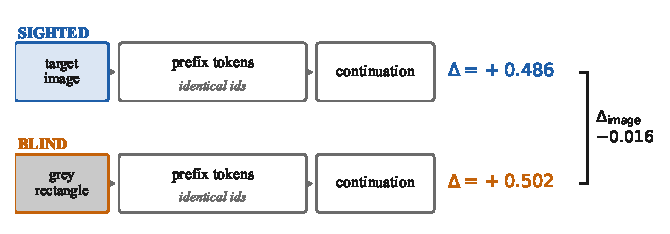
\includegraphics{fig_concept.pdf}\par}
\caption{The design. The sighted and blind rows differ in the image alone; prefix token ids are
bit-identical, so the difference between the two rises is attributable to replacing the image with a
uniform grey field. On \textsc{LLaVA-1.5-7B} that difference is $-0.016$.}
\label{fig:concept}
\end{figure}

\subsection{Models, Decoding and Prompt}
\label{app:modelspec}

Five checkpoints are used; the first two carry every primary number, and the fifth,
\textsc{Qwen3-VL-8B}, is documented separately in Appendix~\ref{app:qwen3}. \textsc{LLaVA-1.5-7B} is
\texttt{llava-1.5-7b-hf} \citep{llava15} in bfloat16 on a single consumer GPU. The second is
\texttt{llava-onevision-qwen2-0.5b-ov-hf} \citep{llavaov}, run with its own tokenizer and its own
chat template. It
differs in language-model family (Qwen2), vision tower (SigLIP), training recipe and resolution
scheme (anyres), and is $7.90\times$ smaller by parameter count. Where the two disagree, the
disagreement is reported rather than pooled.

The two further models in this group were each run under their own registration. \textsc{Qwen2.5-VL-7B} is
\texttt{Qwen/Qwen2.5-VL-7B-Instruct} \citep{qwen25vl} in bfloat16 with its own chat template; its cut, chosen by a
registered census rule before any generation, is $f = 0.230$ (mean prefix $40.7$ tokens) on all
$500$ images. \textsc{Kosmos-2} is \texttt{microsoft/kosmos-2-patch14-224} \citep{kosmos2} in float32, its
checkpoint's own precision. It has no chat template, so its registered prompt is its trained task
string without the grounding marker, \texttt{Describe this image in detail:}, which keeps its output
in plain prose; its census cut is $f = 0.460$ (mean prefix $36.1$ tokens) on $473$ images, after $27$
whose free-running caption was under $32$ tokens were excluded by the registered rule. Both use the
same stimulus assembly, scorer, blinding constant and bootstrap as the first two; their unit counts
and the full census tables are in the released registration records.

Decoding is greedy throughout (\texttt{do\_sample=False}), with no sampling parameters of any kind.
Free-running captions use \texttt{max\_new\_tokens} $=256$; continuations from a supplied prefix use
$384$ in the two-point measurement on \textsc{LLaVA-1.5-7B}, with a $192$-token reconstruction of the
same measurement reported alongside it (Appendix~\ref{app:regime}). Greedy decoding is load-bearing rather than convenient:
because decoding is deterministic, the model's own free-running caption \emph{is} its own
continuation from its own prefix at any cut, so the cut position is matched exactly rather than
approximately.

The prompt is the LLaVA-1.5 v1 conversation format, verbatim, unchanged across every condition:

\begingroup\fontsize{8}{9.5}\selectfont\begin{verbatim}
A chat between a curious human and an artificial intelligence assistant. The
assistant gives helpful, detailed, and polite answers to the human's questions.
USER: <image>
Please describe this image in detail. ASSISTANT:
\end{verbatim}\endgroup

\noindent with one space after the system string and a newline after \texttt{<image>}. Image
preprocessing is the stock LLaVA-1.5 processor, CLIP ViT-L/14-336, with no overrides. Generation is
batched with left padding, batch $16$ for captions and $8$ for continuations.

\textsc{LLaVA-OV-0.5B} differs in one respect that matters for correctness rather than for style.
Under its anyres tiling the prompt length varies per image, from $2{,}088$ to $3{,}714$ tokens, so
the processor itself left-pads; Appendix~\ref{app:gates} gives the gate that catches a hand-rebuilt
attention mask attending to that padding.

\subsection{Images}
\label{app:images}

All images are COCO \texttt{val2017}. An image is eligible if it has at least one instance
annotation, at least one human caption and a readable file. Eligible ids are sorted, $500$ are drawn
without replacement with \texttt{default\_rng(20260817)}, and the draw is re-sorted by image id. The
identical $500$ images are used by every \textsc{LLaVA} condition in the two-point measurement;
\textsc{Kosmos-2} uses $473$ of them (Appendix~\ref{app:modelspec}), the dose grid $499$, and the
generation-regime control a larger sample of $3{,}500$ that nests these $500$. Images whose free-running caption
is shorter than $32$ tokens are excluded from the prefixed conditions; none of the $500$ fell below
this floor, and the observed minimum is $55$ tokens.

One analysis --- the generation-regime control of Appendix~\ref{app:regime} --- extends the sample to
$3{,}500$ images with the original $500$ nested inside, giving $10{,}500$ cells and $21{,}000$ rows.

\subsection{Stimulus Construction}
\label{app:stimulus}

For image $i$, let $L_i$ be the token length of the model's own greedy caption; the cut is
$c_i(f) = \lfloor f \cdot L_i \rfloor$. The primary cut is $f = 0.5$ on \textsc{LLaVA-1.5-7B}, where $c_i(0.5)$ has mean $58.24$ tokens;
the two-point measurement there caps each cell's budget further at the token length of a Localized
Narratives description of the first source image, so the realised budget has mean $44.6$ (sd $13.7$,
range $12$--$87$). On \textsc{LLaVA-OV-0.5B} $f = 0.21$, with mean prefix length $50.272$ tokens. Prefix length is keyed to the image rather than to the condition, so it is identical across
conditions at each cut by construction and the contrast is never a length contrast.

The two conditions of the primary contrast differ in exactly one property of the prefix:

\begin{itemize}
\itemsep0em
\item \texttt{cap1} --- five human COCO captions of \textbf{one} other image.
\item \texttt{cap5} --- five human COCO captions of \textbf{five} different other images.
\end{itemize}

Both are built by the same procedure --- strip terminal periods, shuffle under a per-image seed, join
with \texttt{". "}, tokenize, and slice the token id list to the budget --- except that the one-scene
prefixes use the doubling step described next and the five-scene prefixes do not need it (their
doubling rate is zero by construction). The dose grid rebuilds the one-scene condition without doubling
and lands at $+0.1947$ against $+0.1881$ (Appendix~\ref{app:dose}). Four properties of
that assembler are worth stating precisely, because each has been described loosely elsewhere. If the
joined string tokenizes shorter than the budget it is concatenated to itself verbatim and re-checked,
with a doubling bound of seven; the loop exits on the bound as well as on the budget, so a prefix can
come out shorter than the target. Truncation is a slice of the token id list, so it never cuts inside
a token, but because the tokenizer is subword the boundary can fall mid-word and routinely falls
mid-sentence. The assembler never sees the image: it takes captions, a length and a seed. And the
prefix ids are spliced after the prompt rather than re-encoded with it, so the model is shown a token
sequence that was never produced by tokenizing the full string.

Each image contributes three cells, one per derangement of the partner assignment, giving $1{,}500$
cells over $500$ images in each condition.

\paragraph{Realised rather than nominal dose.} The token budget truncates, so the model does not see
all five assembled units. Across the whole dose grid, units-as-assembled is $5.000$ at every grid
point while units-as-seen is flat at $2.671$--$2.697$; what moves is scenes-as-seen, which rises
$0.999 \rightarrow 1.718 \rightarrow 2.131 \rightarrow 2.414 \rightarrow 2.671$. The manipulation is
described as five-and-five throughout because that is what is held fixed; realised figures are stated
wherever the contrast is quantified.

\paragraph{The dose grid's assembler.} The five-point grid varies the number of distinct source
scenes $S \in \{1,\dots,5\}$ while holding five caption units at every grid point, under quotas
$[5] / [3,2] / [2,2,1] / [2,1,1,1] / [1,1,1,1,1]$, with one assembler throughout, the same per-cell
budget, the same join seed, and zero doubling by construction. Its census kept $1{,}361$ of $1{,}500$
cells across $499$ images ($f_{\mathrm{keep}} = 0.907$).

\paragraph{The blind conditions.} \texttt{cap1g} and \texttt{cap5g} run the identical pipeline with
the target image replaced by a flat mid-grey rectangle at the target's own pixel dimensions, and with
prefix token ids held bit-identical to the corresponding sighted condition. The image-attributable
component is $\dSight = \dPrim - \dBlind$, an algebraic identity in its components; what is empirical
is its magnitude.

\subsection{Object Extraction and Ground Truth}
\label{app:gt}

The scorer is a faithful port of the CHAIR object scorer. The 80-category synonym table is used
verbatim, including its double-word merges (\texttt{sports ball}, \texttt{hot dog},
\texttt{baby <animal>} to \texttt{<animal>}, \texttt{passenger jet} to \texttt{jet}, \texttt{bow tie}
to \texttt{tie}) and the canonical toilet-seat rule. The ground-truth object set $G(i)$ is the union
of image $i$'s segmentation category names and every object mined from that image's human captions
with the same extractor. An object is \emph{in the image} iff its canonical node lies in $G(i)$.

Two portability deviations from the reference implementation are applied identically to every
condition, so their first-order bias cancels in every contrast reported: a regex word tokenizer
(\texttt{[a-z]+} over lowercased text, retaining character offsets) replaces the NLTK tokenizer, and
a rule-based singularizer replaces \texttt{pattern.singularize}. Absolute rates are therefore not
comparable to published CHAIR numbers on these conditions; only within-paper contrasts are.
Appendix~\ref{app:mitig-port} bounds what the two substitutions actually touch at the standard
free-captioning protocol, where the same port reproduces published levels closely; that is one
configuration and does not widen this caveat.

The union construction is deliberately permissive, which makes \rateF{} conservative: a permissive
$G(i)$ can only move objects out of the false class. It also has a consequence that determines the
endpoint choice. A prefix built from an image's own human captions consists of members of $G(i)$ by
construction, so a prefix-copied mention is arithmetically incapable of being scored as a
hallucination. Measured across the grounded conditions of both architectures, $10{,}608$ copied
mentions produced exactly $0$ hallucinations. A per-mention hallucination rate is therefore
structurally undefined on such prefixes, which is why the endpoint below classifies \emph{prefix}
objects and compares carry-forward rates within a condition.

\paragraph{Three constructions.} Every number in the paper is scored under the union. Two further
constructions are used for the sensitivity analysis of Appendix~\ref{app:gtsens}: segmentation-only
($G(i)$ restricted to instance-annotation category names) and caption-only ($G(i)$ restricted to
objects mined from the human captions). The estimator is unmodified across the three; only the
ground-truth dictionary is swapped, and the switch asserts its own union branch equal to the
published $G(i)$ per image.

\subsection{The Endpoint and Its Units}
\label{app:endpoint}

For each (image, condition) pair we extract the object types named in the prefix, $P$, and in the
continuation, $C$. The unit is the pair (image, object type in $P$), deduplicated within a
condition-image, so an object named five times in the prefix contributes exactly one unit, and
carry-forward is the binary event that the type appears anywhere in the continuation. That
deduplication makes the measurement immune to repetition loops in the continuation; it does not
address repetition in the prefix, which is measured directly on the prefix string.

Pooled over units, \rateT{} and \rateF{} are the carry-forward rates for prefix objects in and not in
$G(i)$, and $J = H - F$. Table~\ref{tab:units} gives the realised unit counts.
Because the unit set is fixed by the prefix, and the blind conditions hold prefix token ids
bit-identical, the blind conditions carry the same unit counts as their sighted counterparts by
construction.

\begin{table}[htb]
\caption{Unit counts per condition. A unit is one (image, prefix object type) pair, deduplicated
within a condition-image. The blind conditions share these counts by construction.}
\label{tab:units}
\begin{center}
\small
\begin{tabular}{llrrr}
\toprule
architecture & condition & true units & false units & cells \\
\midrule
\textsc{LLaVA-1.5-7B} & one scene (\texttt{cap1}) & 528 & 2{,}332 & 1{,}500 \\
\textsc{LLaVA-1.5-7B} & five scenes (\texttt{cap5}) & 892 & 4{,}988 & 1{,}500 \\
\textsc{LLaVA-OV-0.5B} & one scene (\texttt{cap1}) & 554 & 2{,}452 & 1{,}500 \\
\textsc{LLaVA-OV-0.5B} & five scenes (\texttt{cap5}) & 1{,}020 & 6{,}308 & 1{,}500 \\
\bottomrule
\end{tabular}
\end{center}
\end{table}

The endpoint $J$ is not pre-registered. It was adopted after CHAIR and the per-mention rate were found
defective on these conditions, for the reason given in Appendix~\ref{app:gt}; this is recorded in
Appendix~\ref{app:prereg} among the specification elements selected in the presence of data.

\subsection{Interval Estimation}
\label{app:boot}

All intervals are paired image-level bootstraps clustered on the image. A replicate resamples the
image ids with replacement, carries \emph{all} of that image's cells into the replicate together,
recomputes both conditions on the resampled set, and the interval is the $2.5$/$97.5$ percentile
range over replicates. Clustering is required rather than optional, because each image contributes
several rows and resampling rows would understate the interval. Multiplicity is preserved --- an
image drawn three times counts three times --- and the resample size is asserted equal to $n$ on
every replicate.

$B = 8000$ for pooled estimates and $B = 4000$ elsewhere. The two-point measurement uses
\texttt{default\_rng(20260830)}; the blind-baseline and signal-detection analyses use seed $20260912$ at
$B = 4000$. Alternate-seed replications are reported for every primary contrast
(Appendix~\ref{app:seeds}).

\subsection{Integrity Gates}
\label{app:gates}

Six gates run before any number is reported. All are pass/abort rather than advisory.

\paragraph{Verification gate.} No pipeline may report a new quantity unless it first reproduces
previously published per-condition rates to within $5\times10^{-3}$. Realised margins: the blind
analysis's positive control reproduced the published $\dPrim$ to $2.9\times10^{-5}$ and
$1.8\times10^{-5}$ on the two architectures; the signal-detection analysis reproduced the unit counts of
Table~\ref{tab:units} exactly with rate deviations of $0.0$ on all four conditions, and reproduced
the published $\Delta$ intervals to $3.3\times10^{-5}$ and $2.5\times10^{-5}$.

\paragraph{Mask-validity gate.} The free-running condition comes straight from the processor, while
the prefixed conditions append prefix token ids and rebuild the batch --- and its attention mask ---
by hand. An error in that hand-built mask would corrupt only the prefixed conditions, and would
manufacture an effect that is large, clean, internally consistent and entirely spurious; nothing in
the resulting numbers would look wrong. The gate is a longest-common-prefix check of the rebuilt
encoding against the processor's own, with a known expected value of $51$, and a batch that fails it
aborts the condition rather than emitting numbers. The risk is acute under \textsc{LLaVA-OV-0.5B}'s
anyres tiling, where the processor itself left-pads.

\paragraph{Attention gate.} Registered, and required to pass before any outcome can be declared. It
compares object recall from the model's own free caption with a real image against the same with flat
grey: $0.839$ and $0.781$ on the two architectures against $0.000$ grey, with an identical-caption
rate of $0.000$ and mean caption length $116.98$ real against $73.01$ grey on \textsc{LLaVA-1.5-7B}.
The grey condition produces different, shorter, object-free captions rather than no captions.

\paragraph{Construction and prefix-identity gates.} Every published prefix is rebuilt from its source
captions under its per-row seed and compared bit-for-bit; realised drift is $0$ of $3{,}000$. Census
checksum drift is $0$. Per-architecture integrity gates on the blind-baseline analysis pass at $1500/1500$ on all
six checks (four conditions present, budget, prefix identity, five-scene zero doubling, cap, self).

\paragraph{Budget and cell-count gates.} Fatal assertions on budget mismatch, cap exceedance,
incomplete cells and cell count against the frozen census; none triggered on any reported run.

\paragraph{Bootstrap multiplicity assertion.} Active in every analysis reported here
(Appendix~\ref{app:boot}, and see Appendix~\ref{app:bootcheck}).

\section{Additional Robustness Analyses}
\label{app:robust}

\begin{figure}[htb]
{\centering
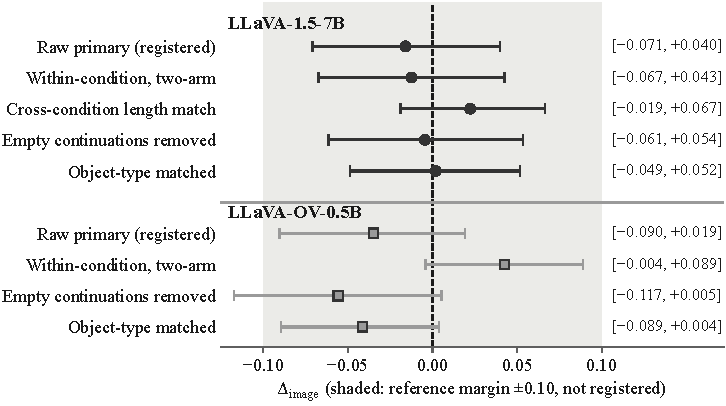
\includegraphics{fig_robustness.pdf}\par}
\caption{The image-attributable component on the two \textsc{LLaVA}-lineage architectures under every
rule in Table~\ref{tab:trunc}, against the $\pm 0.10$ reference margin, which is a reporting choice rather
than a registered bound. One interval, \textsc{LLaVA-OV-0.5B}'s with empty continuations removed,
extends beyond the margin.}
\label{fig:robustness}
\end{figure}


\begin{figure}[htb]
{\centering
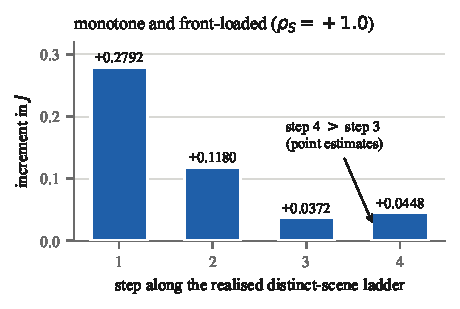
\includegraphics{fig_dose.pdf}\par}
\caption{Increments in $J$ along the realised distinct-scene ladder on \textsc{LLaVA-1.5-7B}. The
first step carries $58\%$ of the rise, so the curve is front-loaded; the fourth step's point estimate
slightly exceeds the third's, so it shows no plateau within the grid. Distinct-type
count and mentions-per-type track the manipulation with the same precision, so the ladder is graded
in a quantity that co-varies with source-scene count rather than isolating it.}
\label{fig:dose}
\end{figure}


Every analysis in this section tests the same quantity: $\dSight = \dPrim - \dBlind$, the part of the
contrast attributable to the image. Figure~\ref{fig:robustness} plots a subset of these rows; the full
set is here, and Figure~\ref{fig:dose} shows the dose-response grid the contrast sits on.

\subsection{Ground-Truth Construction}
\label{app:gtsens}

The null does not depend on how the ground truth was built. Re-scoring all four conditions
under segmentation-only and caption-only definitions, with the estimator unmodified and only the
ground-truth dictionary swapped, gives Table~\ref{tab:gtsens}.

\begin{table}[htb]
\caption{The contrast under three independent ground-truth constructions. The six $\dSight$ point estimates lie between $-0.042$ and
$-0.0156$, and in all six $\dBlind$ exceeds $\dPrim$; intervals are
shown only for the union construction (Table~\ref{tab:trunc}).}
\label{tab:gtsens}
\begin{center}
\small
\begin{tabular}{llrrr}
\toprule
architecture & quantity & union & segmentation only & captions only \\
\midrule
\textsc{LLaVA-1.5-7B}  & $\dPrim$ & $+0.4859$ & $+0.5015$ & $+0.4848$ \\
\textsc{LLaVA-1.5-7B}  & $\dBlind$ & $+0.5019$ & $+0.5172$ & $+0.5126$ \\
\textsc{LLaVA-1.5-7B}  & $\dSight$ & $-0.0160$ & $-0.0156$ & $-0.0279$ \\
\midrule
\textsc{LLaVA-OV-0.5B} & $\dPrim$ & $+0.3780$ & $+0.3682$ & $+0.3743$ \\
\textsc{LLaVA-OV-0.5B} & $\dBlind$ & $+0.4128$ & $+0.4101$ & $+0.4129$ \\
\textsc{LLaVA-OV-0.5B} & $\dSight$ & $-0.0348$ & $-0.0420$ & $-0.0386$ \\
\bottomrule
\end{tabular}
\end{center}
\end{table}

The largest pairwise spread in $\dPrim$ across the three constructions is $0.0167$, which is $3.4\%$
of the effect and roughly a seventh of any one interval's width, and the two architectures' shifts
point in opposite directions --- the signature of noise at this scale rather than of a systematic
construction bias. The arithmetic reason is that reclassification is small and balanced across
conditions: dropping the caption-mined half moves $91$ of $8{,}740$ units ($1.04\%$) on \textsc{LLaVA-1.5-7B} and $109$ of $10{,}334$ ($1.05\%$) on \textsc{LLaVA-OV-0.5B}, affecting $6.4\%$ of union-true units
in \emph{both} conditions on \textsc{LLaVA-1.5-7B} and $7.4\%$ and $6.7\%$ on \textsc{LLaVA-OV-0.5B}. A
construction that reclassified the two conditions at different rates is what would move a contrast
mechanically, and this one does not.

The union row was cross-checked against a second, independently written scorer with its own bootstrap
seed, which returns $0.48587082$ / $0.50151970$ / $0.48475570$ against this analysis's $0.485871$ /
$0.5015$ / $0.4848$.

Two constraints travel with this block. That analysis's own registered decision on the segmentation-only runs is
mechanical rather than substantive --- its gate compares the recomputed contrast against a
union-anchored reference, which a segmentation-only run legitimately misses --- and the six paired
cross-construction differences are point estimates without intervals
(Appendix~\ref{app:repro-limits}). They say how far the constructions agree, not how confidently.

\subsection{Truncation and Length-Matching Rules}
\label{app:trunc}

``Length-matched $\dSight$'' names more than one estimand, and the distinction is consequential, so
every rule we ran is reported. Let $L$ be the per-cell truncation length at which continuations are
re-scored. A \emph{within-condition} rule sets $L$ separately inside the sighted and the blind halves;
a \emph{cross-condition} rule sets one $L$ per cell and applies it to both halves, so the sighted and
blind continuations are evaluated at the same length. Only the cross-condition rule is length-matched
in the sense the phrase implies.

\begin{table}[htb]
\caption{$\dSight$ under each truncation and matching rule. Every interval on the two \textsc{LLaVA}
architectures contains zero. The full ladder was run only on those two; for the other two we give the
registered primary, and for \textsc{Kosmos-2} the length-matched form as well. That match is within
each condition only: blind continuations on \textsc{Kosmos-2} run about $1.7$ times longer than sighted
ones, no sighted-against-blind match was run, and the design cannot separate the image from length. The two
\textsc{Kosmos-2} intervals exclude zero. Rows for the two \textsc{LLaVA} architectures come from the
registration run; the last three, and Table~\ref{tab:blind}, come from the run that measured all four
architectures together. Point estimates agree between the runs; interval endpoints differ in the
third decimal because the bootstrap seeds differ, and both runs are released.}
\label{tab:trunc}
\begin{center}
\footnotesize
\setlength{\tabcolsep}{3pt}
\begin{tabular}{llll}
\toprule
architecture & rule & $\dSight$ & 95\% CI \\
\midrule
\textsc{LLaVA-1.5-7B} & raw, no truncation match (registered primary) & $-0.0160$ & \civ{-0.0708}{+0.0400} \\
\textsc{LLaVA-1.5-7B} & within-condition, two-condition $L$ & $-0.0124$ & \civ{-0.0673}{+0.0427} \\
\textsc{LLaVA-1.5-7B} & cross-condition $L$ & $+0.0223$ & \civ{-0.0190}{+0.0665} \\
\textsc{LLaVA-1.5-7B} & empty continuations removed & $-0.0045$ & \civ{-0.0614}{+0.0536} \\
\textsc{LLaVA-1.5-7B} & type-matched (mention-rate control) & $+0.0019$ & \civ{-0.0488}{+0.0516} \\
\midrule
\textsc{LLaVA-OV-0.5B} & raw, no truncation match (registered primary) & $-0.0348$ & \civ{-0.0905}{+0.0192} \\
\textsc{LLaVA-OV-0.5B} & within-condition, two-condition $L$ & $+0.0426$ & \civ{-0.0041}{+0.0891} \\
\textsc{LLaVA-OV-0.5B} & empty continuations removed & $-0.0557$ & \civ{-0.1172}{+0.0053} \\
\textsc{LLaVA-OV-0.5B} & type-matched (mention-rate control) & $-0.0413$ & \civ{-0.0895}{+0.0040} \\
\midrule
\textsc{Qwen2.5-VL-7B} & raw, no truncation match (registered primary) & $+0.0157$ & \civ{-0.0226}{+0.0552} \\
\textsc{Kosmos-2} & raw, no truncation match (registered primary) & $-0.1028$ & \civ{-0.1677}{-0.0360} \\
\textsc{Kosmos-2} & length-matched & $-0.0873$ & \civ{-0.1502}{-0.0250} \\
\bottomrule
\end{tabular}
\end{center}
\end{table}

The four truncation rules are the raw (unmatched) rule, the
within-condition rule, the cross-condition rule and the empty-continuation rule; the type-matched row
is a matching rule rather than a truncation rule and is discussed in Appendix~\ref{app:mrate}.

The empty-continuation rows run in opposite directions on the two architectures --- closer to zero on
\textsc{LLaVA-1.5-7B}, further from it on \textsc{LLaVA-OV-0.5B}, and containing zero in both --- so the empty-rate asymmetry
between conditions does not explain the null in either direction.

\paragraph{A fifth rule, and why it is not in the table.} A replication analysis computed a
within-condition length match in which $L$ is minimised over \emph{four} conditions, two of which are
not in the contrast, and reports $+0.0395$ \civ{+0.0050}{+0.0754}. We report it here because it is in
the released artefacts and because it is the one length-matched estimate that excludes zero. It
should not be read as a truncation rule for this contrast, for a reason that is checkable
arithmetically. Under that rule the truncation depth is itself a function of the manipulation being
contrasted: removing the image shortens continuations, so the blind half is truncated on $43.7\%$ of
cells against the sighted half's $23.6\%$. The differential shrinkage is $0.1020 - 0.0667 = 0.0353$,
against an observed discrepancy of $+0.0395 - (+0.0042) = +0.0353$, where $+0.0042$
\civ{-0.0335}{+0.0427} is that analysis's cells recomputed under the registered two-condition rule.
The cross-condition version on those cells reads $-0.0140$ \civ{-0.0452}{+0.0172}, the
narrowest of the three. The registered raw primary is untouched by any of this; the replication
analysis computes it on its own cell set, at $-0.0104$ against the registered $-0.0160$.

\subsection{The Mention-Rate Control}
\label{app:mrate}

The strongest competing explanation for the blind null is that a shift in overall mention rate,
rather than blinding, drives it. The threat is real: the one-scene to five-scene increase in mention
count is substantially larger in the blind condition than in the sighted one (sighted minus blind,
$-12.68$ \civ{-14.77}{-10.56}, on \textsc{LLaVA-1.5-7B}).

The pre-registered control holds distinct object \emph{types} fixed rather than mentions, because
carry-forward is set membership and cannot depend on multiplicity. The continuations make the
distinction concrete: on \textsc{LLaVA-1.5-7B} they average $26.59$ object mentions across only
$1.515$ distinct types, so most mentions are re-namings that cannot change any carry outcome. Type-matched, the null holds on
both architectures (Table~\ref{tab:trunc}, last row of each block).

\begin{table}[htb]
\caption{The adversarial re-analysis. The registered verdict passes on all fourteen powered blocks on
\textsc{LLaVA-OV-0.5B} and fails on five of sixteen powered blocks on \textsc{LLaVA-1.5-7B} --- four
mention-count strata in the positive direction and one type-matched block in the negative direction;
both architectures are reported.}
\label{tab:mrate}
\begin{center}
\small
\begin{tabular}{lll}
\toprule
block & estimate & reading \\
\midrule
type-matched, \textsc{LLaVA-1.5-7B} & $+0.0019$ \civ{-0.0488}{+0.0516} & passes \\
type-matched, \textsc{LLaVA-OV-0.5B} & $-0.0413$ \civ{-0.0895}{+0.0040} & passes \\
mention-count strata, \textsc{LLaVA-1.5-7B} & $+0.093$ to $+0.107$, four blocks & \textbf{fails} \\
type-matched block ($\tau = 2$), \textsc{LLaVA-1.5-7B} & $-0.0688$ \civ{-0.1343}{-0.0057} & \textbf{fails} \\
all fourteen powered blocks, \textsc{LLaVA-OV-0.5B} & --- & passes \\
repeat-mention probe, \textsc{LLaVA-1.5-7B} & $+0.1144$ \civ{+0.0519}{+0.1734} & diagnostic \\
conditioning on types directly & $+0.002$ & diagnostic \\
\bottomrule
\end{tabular}
\end{center}
\end{table}

Four mention-count-stratified blocks on \textsc{LLaVA-1.5-7B} come out positive, in the direction
pre-specified as adverse. We report the failure rather than amend the rule, and we report the
diagnostic that indicates why it occurs. Stratifying on repeat mentions alone --- the quantity
$\mathrm{mentions} - \mathrm{types}$, which by construction cannot change any carry outcome ---
reproduces the effect more strongly ($+0.1144$) than the mention-count stratification does, while
conditioning on types directly gives $+0.002$. A variable incapable of affecting the endpoint
therefore reproduces the effect better than the variable of interest, which is what one expects if
the stratifier is a proxy for something else. It is: every mention stratum above roughly sixteen on
\textsc{LLaVA-1.5-7B} is entirely cap-truncated, so high mention count there marks ``reached the
token cap and looped'' rather than verbosity.

\paragraph{The smallest ratio across strata.} Across all adequately powered blocks, the smallest point
estimate of $\dBlind / \dPrim$ is $0.7333$ on \textsc{LLaVA-1.5-7B} and $0.9074$ on \textsc{LLaVA-OV-0.5B}. These
are minima of point estimates, not confidence bounds; the ratio on the full sample is $1.033$
\civ{0.922}{1.155}. What we claim is that the image-attributable component of $J$ is null at our
power --- not that the image adds nothing detectable,
which Appendix~\ref{app:dprime-table} shows directly to be false.

\subsection{One Block That Runs in Our Favour and Is Unexplained}
\label{app:oddblock}

A type-restricted block on \textsc{LLaVA-1.5-7B} returns $\dSight = -0.0688$
\civ{-0.1343}{-0.0057} and is systematic rather than sampling noise: it sits at the $0.27$th
percentile of same-size random subsets of the same cells. The repeat-mention probe does not reproduce
it, no truncation account explains it, and \textsc{LLaVA-OV-0.5B} shows nothing comparable (the
corresponding block sits at the $55.5$th percentile). A negative $\dSight$ means the image acts in a
direction nobody predicted, and it flatters the conclusion of this paper, which is a reason for more
suspicion rather than less. The cells this block excludes --- those in which the five-caption prefix raised the count of distinct
types sharply --- return $\dSight = +0.1264$ \civ{+0.0143}{+0.2432}, so the pooled null combines
subgroups of opposite sign; this split was examined after the fact. Both halves are defined by a
post-treatment quantity, so neither half is a causal contrast and no re-weighting of these data will settle it; resolving it
requires a design that manipulates prefix type-content directly.

\subsection{Generation Regime}
\label{app:regime}

The five-scene condition generates longer continuations and reaches the generation cap more often
(share at the budget $0.679$ against the one-scene condition's $0.447$), so a control that removes
truncation from the comparison is necessary. Requiring that \emph{neither} condition reach the budget
keeps $21.5\%$ of cells at $500$ images ($323$ of $1{,}500$) and drops the true-unit count to $75$
against a registered floor of $100$; the contrast is then $+0.4667$ \civ{+0.3129}{+0.6134} and
underpowered by its own rule. Raising the budget from $192$ to $384$ tokens does not fix this ---
truncation barely moves (share at the budget $0.448 / 0.677$ at $384$ against $0.447 / 0.679$ at
$192$). Adding images does.

\begin{table}[htb]
\caption{The generation-regime control at power: the contrast measured only on cells in which neither
condition reached the generation cap, at $3{,}500$ images. On a subset where neither condition reached the budget, greedy decoding makes the $192$- and $384$-token continuations identical, so that row is a determinism check rather than an independent replication.}\label{tab:regime}
\begin{center}
\footnotesize
\setlength{\tabcolsep}{4pt}
\begin{tabular}{llll}
\toprule
estimate & $\Delta$ & 95\% CI & width \\
\midrule
both conditions untruncated, $3{,}500$ images (primary) & $+0.3460$ & \civ{+0.2849}{+0.4058} & $0.1209$ \\
the same, length-matched & $+0.1999$ & \civ{+0.1462}{+0.2524} & $0.1062$ \\
the same, $192$-token reconstruction (determinism check) & $+0.3460$ & \civ{+0.2849}{+0.4058} & $0.1209$ \\
the same, alternate bootstrap seed & $+0.3460$ & \civ{+0.2876}{+0.4050} & $0.1174$ \\
composition control, base-rate tertiles & $+0.1994$ & \civ{+0.1059}{+0.2897} & $0.1838$ \\
composition control, shared object types & $+0.3496$ & \civ{+0.2923}{+0.4168} & $0.1245$ \\
all cells, raw, $3{,}500$ images & $+0.4719$ & \civ{+0.4507}{+0.4928} & $0.0421$ \\
all cells, length-matched, $3{,}500$ images & $+0.3679$ & \civ{+0.3478}{+0.3872} & $0.0394$ \\
original $500$ images only, both untruncated (descriptive) & $+0.4663$ & \civ{+0.3139}{+0.6124} & $0.2985$ \\
\bottomrule
\end{tabular}
\end{center}
\end{table}

The control passes: interval width $0.1209$ against a registered ceiling of $0.130$, true units
$466 / 914$ against a floor of $100$, on $2{,}089$ of $10{,}500$ cells. The untruncated subset is
short-continuation by construction (mean $28.9$ tokens in the one-scene condition against $40.3$ in
the five-scene condition), so a positive verdict says the effect exists \emph{within} the
regime-matched population and no more.

Two facts bear on this estimate. The confirmatory estimate is $26\%$ below the
underpowered $500$-image estimate that motivated running it, and the confirmatory interval
\emph{excludes} that point estimate while the underpowered interval comfortably contains the
confirmatory one. An arithmetic decomposition of the reported unit counts puts the $3{,}000$
extension images alone at $+0.3237$; that figure carries no interval and enters no registered decision, and
is given because it makes the shrinkage concrete. The frozen original stimulus set replicates cleanly
alongside it: the original all-cells contrast of $+0.4859$ reproduces at $+0.4877$
\civ{+0.4298}{+0.5434} on the regenerated cells, and the regenerated untruncated subset gives $+0.4663$
on $321$ cells at $76$ true units against the original's $+0.4667$ on $323$ cells at $75$.

The same control is unevaluated on \textsc{LLaVA-OV-0.5B}, where the untruncated subset reaches $90$
true units on $287$ of $1{,}500$ cells against the same floor of $100$. It points the same way as
that architecture's primary ($+0.2830$) and may not be read as support. The dose grid's own regime
control is likewise unevaluated: truncation rises monotonically with the dose
(share at the budget $0.436 \rightarrow 0.655$, Spearman $\rho = +1.0$), and the registered
all-untruncated control reaches $150$ cells with true-unit counts between $29$ and $72$ against a floor
of $100$.

\subsection{Seeds and Reconstructions}
\label{app:seeds}

\begin{table}[htb]
\caption{Alternate-seed and alternate-budget replications of the primary contrasts.}
\label{tab:seeds}
\begin{center}
\small
\begin{tabular}{lll}
\toprule
quantity & estimate & 95\% CI \\
\midrule
$\dPrim$, \textsc{LLaVA-OV-0.5B}, alternate bootstrap seed & $+0.3780$ & \civ{+0.3233}{+0.4352} \\
regime control, alternate bootstrap seed & $+0.3460$ & \civ{+0.2876}{+0.4050} \\
regime control, $192$-token reconstruction & $+0.3460$ & \civ{+0.2849}{+0.4058} \\
forced-choice contrast, alternate bootstrap seed & $-0.0095$ & \civ{-0.0312}{+0.0118} \\
\bottomrule
\end{tabular}
\end{center}
\end{table}

\section{Signal-Detection Derivation}
\label{app:sdt}

\begin{figure}[htb]
{\centering
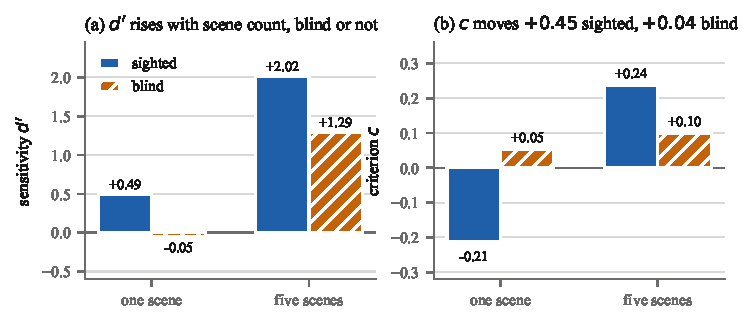
\includegraphics{fig_sdt.pdf}\par}
\caption{Signal-detection decomposition on \textsc{LLaVA-1.5-7B}. Sensitivity rises with scene count
whether or not the image is present; the criterion moves mainly when it is.}
\label{fig:sdt}
\end{figure}


This section derives the relationship the main text relies on, and states the assumptions it needs;
Figure~\ref{fig:sdt} shows the operating points the derivation is evaluated at.
Write $H$ for the carry-forward rate on prefix objects present in the image and
$F$ for the rate on absent ones. Let $\Phi$ be the standard normal distribution function,
$\varphi$ its density, and $Z = \Phi^{-1}$.

\subsection{The Reparameterisation}

The three summaries are
\begin{align}
J &= H - F, \label{eq:appJ}\\
d' &= Z(H) - Z(F), \label{eq:dprime}\\
c &= -\tfrac{1}{2}\left[ Z(H) + Z(F) \right]. \label{eq:crit}
\end{align}
Equations~\ref{eq:dprime}--\ref{eq:crit} invert exactly:
\begin{equation}
Z(H) = \tfrac{d'}{2} - c, \qquad Z(F) = -\tfrac{d'}{2} - c,
\end{equation}
so that
\begin{equation}
H = \Phi\!\left(\tfrac{d'}{2} - c\right), \qquad
F = \Phi\!\left(-\tfrac{d'}{2} - c\right), \qquad
J(d',c) = \Phi\!\left(\tfrac{d'}{2} - c\right) - \Phi\!\left(-\tfrac{d'}{2} - c\right).
\label{eq:Jdc}
\end{equation}
The map $(H,F) \mapsto (d',c)$ is a bijection from $(0,1)^2$ onto $\mathbb{R}^2$: two observed rates,
two parameters. On a single operating point the equal-variance Gaussian model is therefore
\emph{saturated}. Nothing is estimated beyond the two rates, and $d'$ and $c$ are re-expressions of
them rather than fits --- a point we return to in Appendix~\ref{app:sdt-assumptions}, because it cuts
both ways.

\subsection{$J$ Is Not Invariant to the Criterion}
\label{app:sdt-noninvariance}

Differentiating \eqref{eq:Jdc} in $c$ at fixed $d'$, and using the symmetry of $\varphi$,
\begin{equation}
\frac{\partial J}{\partial c}
 = \varphi\!\left(\tfrac{d'}{2} + c\right) - \varphi\!\left(\tfrac{d'}{2} - c\right)
 = -\frac{2}{\sqrt{2\pi}}\,
   \exp\!\left(-\frac{d'^2/4 + c^2}{2}\right) \sinh\!\left(\frac{c\,d'}{2}\right).
\label{eq:appdJdc}
\end{equation}
This vanishes if and only if $c\,d' = 0$. For $d' > 0$ it is strictly negative for $c > 0$ and
strictly positive for $c < 0$, so at fixed $d'$ the statistic $J$ increases in $c$ on $c < 0$,
decreases on $c > 0$, and attains a unique interior maximum at $c = 0$:
\begin{equation}
J^{*}(d') \;=\; \max_{c}\, J(d',c) \;=\; 2\Phi\!\left(\tfrac{d'}{2}\right) - 1,
\qquad\text{so}\qquad
J(d',c) \le 2\Phi\!\left(\tfrac{d'}{2}\right) - 1
\label{eq:Jmax}
\end{equation}
with equality if and only if $c = 0$. The right-hand side of \eqref{eq:Jmax} is Youden's index of the
equal-variance Gaussian ROC with separation $d'$.

Equation~\ref{eq:Jmax} is the precise sense in which a present-minus-absent rate both is and is not
criterion-free. Youden's index, as a summary of an ROC \emph{curve}, is criterion-free by
definition: it is the maximum over operating points, and a maximum does not depend on where on the
curve one happens to sit. A present-minus-absent rate measured at a single, uncontrolled operating
point equals that maximum only when the operating point happens to be unbiased, and otherwise
under-reports it by an amount that is itself a function of the criterion. Free generation supplies no
mechanism that pins the operating point at $c = 0$, and Appendix~\ref{app:dprime-table} shows that in
our data it is not pinned there.

The local behaviour explains why the confusion is durable. Since $\varphi'(x) = -x\varphi(x)$,
\begin{equation}
\left.\frac{\partial^2 J}{\partial c^2}\right|_{c=0} = -\,d'\,\varphi\!\left(\tfrac{d'}{2}\right),
\qquad\text{hence}\qquad
J(d',c) \;=\; 2\Phi\!\left(\tfrac{d'}{2}\right) - 1
 \;-\; \tfrac{1}{2}\, d'\, \varphi\!\left(\tfrac{d'}{2}\right) c^{2} \;+\; O(c^{4}).
\label{eq:expand}
\end{equation}
The leading criterion dependence is quadratic, not linear. A criterion shift confined to a
neighbourhood of the unbiased point costs $J$ only at second order, which is why the statistic is
routinely described as bias-corrected. A criterion shift between two points that are not symmetric
about zero moves $J$ at first order, with the slope given by \eqref{eq:appdJdc}.

\subsection{The Conditions Under Which It Would Be Invariant}
\label{app:sdt-conditions}

From \eqref{eq:appdJdc}, $J$ is \emph{exactly} invariant to the criterion in three cases and no others.

\begin{enumerate}
\itemsep0em
\item $d' = 0$, where $J \equiv 0$ for every $c$. This is the degenerate case, not a useful one.
\item $c$ held fixed across the compared conditions. Then $\Delta J$ is a function of $\Delta d'$ and
of the common $c$ alone. This is the condition an experiment can actually arrange, and arranging it
is what a response-rate control does.
\item Criteria symmetric about the unbiased point, $c_2 = -c_1$, since $J$ is even in $c$ at fixed
$d'$.
\end{enumerate}

\noindent It is \emph{approximately} invariant whenever
$\tfrac{1}{2}d'\varphi(d'/2)\,c^2$ falls below the resolution of interest. The coefficient
$d'\varphi(d'/2)$ rises from $0.193$ at $d' = 0.5$ to $0.484$ at $d' = 2.0$. At $d' = 1.5$, exact
evaluation of \eqref{eq:Jdc} gives a cost of $0.0023$ in $J$ for a criterion displacement of
$|c| = 0.1$ and $0.054$ for $|c| = 0.5$.

\paragraph{The complementary exact statement, which needs no distributional assumption.} On the rate
scale, if both rates receive a common additive shift $\delta$, then $J$ is exactly unchanged while
$d'$ is not, unless $H = F$. On the probit scale the roles reverse: a pure criterion move at fixed
$d'$ is a common additive shift of $Z(H)$ and $Z(F)$, under which $d'$ is exactly unchanged while $J$
is not, unless $c = 0$. The two summaries are exactly invariant to different perturbations, and
neither is invariant to the other's. Which of those two invariances an evaluation wants is a
substantive choice about what the evaluation is for; reporting only $J$ makes that choice silently.

\subsection{Where the Equal-Variance Gaussian Assumption Is and Is Not Warranted}
\label{app:sdt-assumptions}

The assumption is warranted in three respects and unwarranted in four, and we state both halves
because the derivation above is only as good as the model it sits in.

\paragraph{Warranted.} \emph{(i) Nothing is fitted.} On one operating point the map of
\eqref{eq:Jdc} is a bijection, so $d'$ and $c$ consume exactly the information in $H$ and $F$. Every
statement above is checkable directly from the two rates, and the values in
Table~\ref{tab:sdt-audit} are verified to be so. \emph{(ii) No boundary pathology.} Rates are
log-linear corrected, $(\mathrm{hits}+0.5)/(n_{\mathrm{signal}}+1)$, applied unconditionally to every
condition so that none is selectively corrected; no boundary-rate events were recorded, so no $Z$ is
evaluated at an endpoint. \emph{(iii) The qualitative conclusion is link-free.} Under a logit link
the same two contrasts read $+0.4207$ \civ{+0.1498}{+0.6911} on the discriminability coordinate and
$+0.6953$ \civ{+0.5448}{+0.8478} on the criterion coordinate, so sign and exclusion of zero are not
probit artefacts. More generally, the argument of Appendix~\ref{app:sdt-conditions} needs only that
the reparameterisation separate a discriminability coordinate from a propensity coordinate; the
Gaussian choice fixes which coordinates, not whether the confound exists.

\paragraph{Not warranted.} \emph{(i) There is no z-ROC.} Equal variance is testable only
with several criterion points per condition. A binary carry outcome at one operating point supplies a
single $(H,F)$ pair, so the model is saturated and the equal-variance assumption carries no degree of
freedom against which it could fail. Unequal variance would change the numerical values of $d'$ and
$c$; it would not change the fact that $J$ depends on both. \emph{(ii) There is no explicit decision
threshold.} Carry-forward is not a thresholded judgement on a latent evidence axis. It is an emergent
property of autoregressive generation: whether a type named in the prefix reappears anywhere in a
continuation produced under a fixed token budget. The latent-variable story is a description of two
rates, not a mechanism claim, and should not be read as one. \emph{(iii) Units within an image are
not independent.} Object types drawn from one prefix compete for one continuation and one token
budget. Deduplication removes repetition \emph{within} a continuation but not this competition. The
intervals respect the dependence, since they cluster on the image
(Appendix~\ref{app:boot}); the Gaussian model's unit-level independence does not. \emph{(iv) The
budget binds.} With shares at the budget of $0.447$ and $0.679$ in the two conditions of \textsc{LLaVA-1.5-7B}, a large fraction of continuations end at the budget, so a unit's carry probability depends
on how many other units compete for the remaining budget. A capacity constraint of that kind is not
representable as a threshold on a per-unit evidence variable, and it cannot be absorbed into either
$d'$ or $c$.

Finally, the cancellation of a response-propensity shift out of $J$ is \emph{exact} only under an
additive shift of both rates, and only \emph{approximate} under an equal-variance Gaussian model of
the same shift. The same qualification attaches to the component analysis of
Appendix~\ref{app:dprime-table}.



\subsection{Operating Points in Signal-Detection Coordinates}
\label{app:zroc}

Figure~\ref{fig:zroc} places the four cells of the main contrast in $z$-coordinates, where a change
that moves along a constant-$d'$ contour is a pure threshold shift and one that crosses contours is a
change in separability. It is a reading aid for Table~\ref{tab:report} and adds no new quantity. In panel~(a)
both arms cross contours between the one-scene and five-scene conditions ($d'$ rises $1.53$ sighted
and $1.35$ blind), so the rise is largely a change of separability with or without the image. In
panel~(b) PAI moves nearly parallel to the contours, a large $\Delta c$ beside a $\Delta d'$ whose
interval contains zero.

\begin{figure}[htb]
{\centering
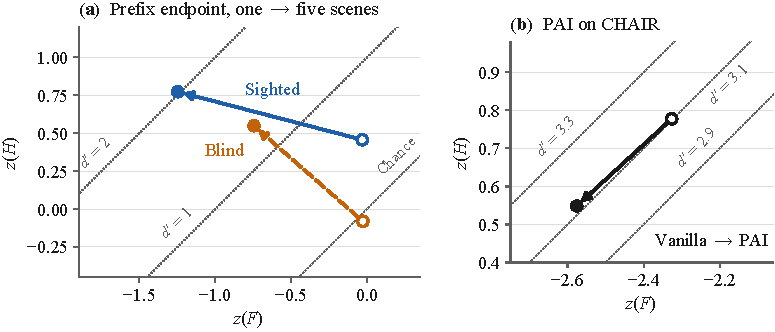
\includegraphics{fig_zroc.pdf}\par}
\caption{Operating points in $z$-coordinates. Dotted lines hold $d' = z(H) - z(F)$ constant, so height
above the chance diagonal is separation and movement parallel to it is a change of threshold.
\textbf{(a)} The scene-count rise on \textsc{LLaVA-1.5-7B}, from one scene (open) to five (filled),
moves away from the diagonal almost as far without the image as with it (post hoc for these
conditions). \textbf{(b)} PAI on standard CHAIR moves almost parallel to the diagonal: on this probit
scale the threshold changes and separation does not, although a logit separation measure does rise
(Section~\ref{sec:mitigation}).}
\label{fig:zroc}
\end{figure}

\subsection{Numerical Audit at the Reported Operating Points}
\label{app:sdt-audit}

Table~\ref{tab:sdt-audit} evaluates \eqref{eq:Jdc}, \eqref{eq:appdJdc} and \eqref{eq:Jmax} at the
per-condition $d'$ and $c$ reported for \textsc{LLaVA-1.5-7B}, and compares the result against the
independently measured $J$. The reconstruction is not a new measurement, but the identity
\eqref{eq:Jdc} applied to values reported elsewhere in this paper, and it is included because a
reviewer can and should check it.

\begin{table}[htb]
\caption{Reconstruction of the measured $J$ from the reported $d'$ and $c$ on \textsc{LLaVA-1.5-7B},
via $J(d',c) = \Phi(d'/2 - c) - \Phi(-d'/2 - c)$. Residuals are at the resolution of the
four-decimal $d'$ and $c$ inputs. $J^{*}$ is the criterion-free Youden index at the same $d'$.}
\label{tab:sdt-audit}
\begin{center}
\footnotesize
\setlength{\tabcolsep}{3.5pt}
\begin{tabular}{lrrrrrrr}
\toprule
condition & $d'$ & $c$ & $J(d',c)$ & meas.\ $J$ & residual & $J^{*}(d')$ & $\partial J/\partial c$ \\
\midrule
sighted, one scene   & $+0.4861$ & $-0.2130$ & $+0.1878$ & $+0.18814$ & $-0.00033$ & $+0.1920$ & $+0.039$ \\
sighted, five scenes & $+2.0183$ & $+0.2371$ & $+0.6736$ & $+0.67401$ & $-0.00038$ & $+0.6871$ & $-0.113$ \\
blind, one scene     & $-0.0549$ & $+0.0532$ & $-0.0219$ & $-0.02191$ & $+0.00004$ & $-0.0219$ & $+0.001$ \\
blind, five scenes   & $+1.2918$ & $+0.0975$ & $+0.4797$ & $+0.47997$ & $-0.00032$ & $+0.4817$ & $-0.041$ \\
\bottomrule
\end{tabular}
\end{center}
\end{table}

Three things follow, and the third is the one that matters.

First, the reconstruction reproduces all four measured gaps to within $4\times10^{-4}$, which is the
resolution of the quoted inputs. The signal-detection and $J$ analyses are therefore describing
the same four cells, and the reader may treat $(d', c)$ and $(\rateT, \rateF)$ as interchangeable
coordinates on this data.

Second, the operating points are close to, but not at, the unbiased point. The measured $J$ falls
short of the criterion-free Youden index $J^{*}$ by $0.0039$, $0.0131$, $0.0000$ and $0.0017$ in the
table's row order (for the blind one-scene cell, where $d' < 0$, $J^{*}$ is the most negative value
attainable rather than the largest), so at these operating points $J$ under-reports the discriminability available at the
same $d'$, by an amount that is itself a function of the criterion. This is the second-order regime
of \eqref{eq:expand}.

Third, decomposing $\dSight$. Evaluating \eqref{eq:Jdc} with the reported $d'$ values but $c$ set to
zero in all four cells gives contrasts of $+0.4951$ sighted and $+0.5036$ blind, so
$\dSight = -0.0085$ on the discriminability coordinate alone; the criterion terms supply the
remaining $-0.0075$ of the reported $-0.0160$. On these data the \emph{movement} of $J$ is
therefore carried predominantly by $d'$, and the criterion coordinate contributes about $0.007$ to a
contrast of $0.486$. This sharpens the diagnosis rather than softening it. The
criterion moves substantially in the sighted conditions, from $-0.213$ to $+0.237$, and barely at all
in the blind ones, from $+0.053$ to $+0.098$, and the image-attributable component of the criterion
contrast is $+0.4057$ \civ{+0.3157}{+0.4957} --- \emph{larger} than the image-attributable component
of discriminability, $+0.1855$ \civ{+0.0252}{+0.3463}. Both of those image effects are invisible in
$J$: the criterion effect because $J$ is stationary in $c$ near the unbiased point
(\eqref{eq:expand}), and the discriminability effect because the map $d' \mapsto 2\Phi(d'/2)-1$ is
concave, its slope $\varphi(d'/2)$ falling from $0.387$ at $d' = 0.5$ to $0.242$ at $d' = 2.0$, so
the same increment in $d'$ buys less $J$ at the higher $d'$ at which the sighted conditions sit. An
endpoint that is stationary in one coordinate by construction and compressive in the other is not a
measure of either.

\section{Additional Model Results}
\label{app:models}


\begin{table}[htb]
\caption{The rise with and without the image, for the four architectures in this group. The blind rise is
positive in every case. The image-attributable component lies within $\pm 0.10$ on the first three and
excludes zero on \textsc{Kosmos-2}, where removing the image \emph{increases} the rise.
$^{\dagger}$\textsc{Qwen2.5-VL-7B} produces a median continuation of four tokens (five on its blind
one-scene arm), which leaves a carry-forward endpoint almost nothing to register. Its registration
states that it does not constitute a replication, and the main text does not count it. We did not
verify that this length reflects the model rather than our prompt and chat template for it, so we do
not interpret the row.}
\label{tab:blind}
\begin{center}
\small
\begin{tabular}{lrrl}
\toprule
Architecture & Sighted $\dPrim$ & Blind $\dBlind$ & $\dSight$ \\
\midrule
\textsc{LLaVA-1.5-7B} & $+0.4859$ & $+0.5019$ & $-0.0160$ \civ{-0.0701}{+0.0399} \\
\textsc{LLaVA-OV-0.5B} & $+0.3780$ & $+0.4128$ & $-0.0348$ \civ{-0.0906}{+0.0179} \\
\textsc{Qwen2.5-VL-7B}$^{\dagger}$ & $+0.1598$ & $+0.1441$ & $+0.0157$ \civ{-0.0226}{+0.0552} \\
\textsc{Kosmos-2} & $+0.2148$ & $+0.3176$ & $\mathbf{-0.1028}$ \civ{-0.1677}{-0.0360} \\
\bottomrule
\end{tabular}
\end{center}
\end{table}


\subsection{Per-Condition Rates and Contrasts}
\label{app:percond}

\begin{table}[htb]
\caption{Per-condition carry-forward rates and gaps. Unit counts are in Table~\ref{tab:units}; the
blind conditions share them by construction.}
\label{tab:percond}
\begin{center}
\small
\begin{tabular}{lllll}
\toprule
architecture & condition & \rateT{} & \rateF{} & $J$ \\
\midrule
\textsc{LLaVA-1.5-7B} & sighted, one scene & $0.6761$ & $0.4880$ & $+0.1881$ \civ{+0.1416}{+0.2362} \\
\textsc{LLaVA-1.5-7B} & sighted, five scenes & $0.7803$ & $0.1063$ & $+0.6740$ \civ{+0.6410}{+0.7072} \\
\textsc{LLaVA-1.5-7B} & blind, one scene & $0.4678$ & $0.4897$ & $-0.0219$ \\
\textsc{LLaVA-1.5-7B} & blind, five scenes & $0.7085$ & $0.2285$ & $+0.4800$ \civ{+0.4441}{+0.5148} \\
\midrule
\textsc{LLaVA-OV-0.5B} & sighted, one scene & $0.5578$ & $0.5171$ & $+0.0406$ \\
\textsc{LLaVA-OV-0.5B} & sighted, five scenes & $0.5471$ & $0.1284$ & $+0.4187$ \\
\textsc{LLaVA-OV-0.5B} & blind, one scene & $0.2058$ & $0.3230$ & $-0.1172$ \\
\textsc{LLaVA-OV-0.5B} & blind, five scenes & $0.3922$ & $0.0965$ & $+0.2956$ \civ{+0.2632}{+0.3271} \\
\bottomrule
\end{tabular}
\end{center}
\end{table}

A model that cannot see the image at all posts a large positive $J$: $+0.4800$ and $+0.2956$ in the
five-scene blind conditions of the two architectures. Table~\ref{tab:contrasts} gives the contrasts
and their pre-registered controls.

\begin{table}[htb]
\caption{The primary contrast and its controls on both architectures. The two point estimates differ
($+0.4859$ against $+0.3780$), but their raw intervals overlap narrowly, as do the length-matched
ones.}
\label{tab:contrasts}
\begin{center}
\small
\begin{tabular}{lll}
\toprule
contrast & $\Delta$ & 95\% CI \\
\midrule
\multicolumn{3}{l}{\textsc{LLaVA-1.5-7B}} \\
\quad primary, raw & $+0.4859$ & \civ{+0.4283}{+0.5417} \\
\quad co-primary, length-matched & $+0.3558$ & \civ{+0.3045}{+0.4082} \\
\quad composition control, base-rate tertiles & $+0.3327$ & \civ{+0.2212}{+0.4367} \\
\quad composition control, shared object types & $+0.4696$ & \civ{+0.4153}{+0.5261} \\
\quad blind & $+0.5019$ & \civ{+0.4441}{+0.5565} \\
\quad $\dBlind / \dPrim$ & $1.033$ & \civ{0.922}{1.155} \\
\midrule
\multicolumn{3}{l}{\textsc{LLaVA-OV-0.5B}} \\
\quad primary, raw & $+0.3780$ & \civ{+0.3213}{+0.4333} \\
\quad co-primary, length-matched & $+0.2871$ & \civ{+0.2375}{+0.3365} \\
\quad object-type-matched & $+0.3655$ & \civ{+0.3129}{+0.4276} \\
\quad doubled prefixes removed & $+0.3733$ & \civ{+0.3162}{+0.4310} \\
\quad empty continuations removed & $+0.3905$ & \civ{+0.3311}{+0.4478} \\
\quad blind & $+0.4128$ & \civ{+0.3609}{+0.4640} \\
\quad $\dBlind / \dPrim$ & $1.092$ & \civ{0.954}{1.265} \\
\bottomrule
\end{tabular}
\end{center}
\end{table}

\paragraph{The doubling check.} The assembler of Appendix~\ref{app:stimulus} reaches its budget by
self-concatenation, and on \textsc{LLaVA-OV-0.5B} the budget is close to twice what five COCO
captions fill, so the one-scene condition's prefixes are frequently doubled text while the five-scene
condition's are not. Doubling is detected on the prefix string itself --- whether its leading half
reappears verbatim, plus an $8$-gram distinctness floor --- rather than inferred from the assembler's
counter. Removing every doubled prefix leaves the contrast at $+0.3733$ \civ{+0.3162}{+0.4310}
against a raw $+0.3780$ \civ{+0.3213}{+0.4333}, so \textsc{LLaVA-OV-0.5B}'s result is not a
duplication artefact.

\paragraph{Why the composition controls are load-bearing.} Five source scenes contribute roughly
twice the prefix objects of one: a mean of $3.92$ distinct object types against $1.91$ on \textsc{LLaVA-1.5-7B}. Length matching is likewise not optional, because the five-scene condition generates
longer text and reaches the budget far more often ($0.679$ against $0.447$); it costs
$27\%$ of the effect and threatens neither its sign nor its power.

\paragraph{What the composition controls do not fix.} Every composition control in this paper matches
on the object \emph{set}, and the set operation discards per-occurrence counts, so these controls fix
which object types appear and never how often each is stated. Measured on the frozen prefixes
themselves, with no model in the loop (Table~\ref{tab:census}), total object mentions are nearly
conserved across the two conditions while the count of distinct types roughly doubles, so mentions
per type falls reciprocally. That quantity is unmatched in every contrast above, and it is part of
the reason the contrast is named by its manipulation rather than by a mechanism.

\begin{table}[htb]
\caption{Stimulus-side census on the frozen prefixes of \textsc{LLaVA-1.5-7B}, $1{,}500$ cells, no
model in the loop.}
\label{tab:census}
\begin{center}
\small
\begin{tabular}{lrr}
\toprule
per prefix & one scene & five scenes \\
\midrule
total object mentions & $4.933$ & $4.829$ \\
distinct object types & $1.907$ & $3.920$ \\
mentions per type & $2.623$ & $1.248$ \\
fraction of prefixes containing a restated type & $0.902$ & $0.539$ \\
\bottomrule
\end{tabular}
\end{center}
\end{table}

\subsection{The Image's Contribution Within Each Condition}
\label{app:withincond}

The blind null concerns the \emph{change} in the image's contribution between conditions, not whether
the image contributes. Table~\ref{tab:withincond} gives the contribution itself: sighted minus blind
$J$ within each condition, from the same run and bootstrap ($B = 4000$) as Table~\ref{tab:dprime}.
It is large and excludes zero in all four cells, which shows the design detects image effects of this
size; it is nearly equal across conditions, which is why $\dSight$ is null. The image's contribution to
$d'$ also excludes zero in every cell (Table~\ref{tab:dprime}) but is \emph{not} equal across
conditions, and the image's contributions to \rateT{} and \rateF{} separately differ by condition and
offset in $J$ (Table~\ref{tab:report}).

\begin{table}[htb]
\caption{The image's contribution to $J$ within each condition: sighted minus blind, with $95\%$
clustered bootstrap intervals. $\dSight$ is the five-scene row minus the one-scene row.}
\label{tab:withincond}
\begin{center}
\small
\begin{tabular}{llll}
\toprule
architecture & condition & sighted $-$ blind & 95\% CI \\
\midrule
\textsc{LLaVA-1.5-7B}  & one scene   & $+0.2100$ & \civ{+0.1635}{+0.2584} \\
\textsc{LLaVA-1.5-7B}  & five scenes & $+0.1940$ & \civ{+0.1591}{+0.2316} \\
\textsc{LLaVA-OV-0.5B} & one scene   & $+0.1579$ & \civ{+0.1119}{+0.2041} \\
\textsc{LLaVA-OV-0.5B} & five scenes & $+0.1230$ & \civ{+0.0921}{+0.1538} \\
\bottomrule
\end{tabular}
\end{center}
\end{table}

\subsection{Which Rate Moves}
\label{app:halves}

\begin{table}[htb]
\caption{Decomposition of the contrast into its two rates, at matched length on \textsc{LLaVA-1.5-7B}. Each row is the five-scene value minus the one-scene value.}
\label{tab:halves}
\begin{center}
\small
\begin{tabular}{lll}
\toprule
half & $\Delta$ & 95\% CI \\
\midrule
\rateT{} & $-0.0301$ & \civ{-0.0760}{+0.0153} \\
\rateF{} & $-0.3859$ & \civ{-0.4086}{-0.3650} \\
log-odds interaction & $+2.2065$ & \civ{+1.9565}{+2.4609} \\
\bottomrule
\end{tabular}
\end{center}
\end{table}

At matched length the false-object carry-forward rate falls from $0.463$ to $0.077$ --- a factor of
six --- while the true-object rate does not move at a resolution this design can detect. In raw,
unmatched data \textsc{LLaVA-1.5-7B}'s \rateT{} also rises ($0.6761 \rightarrow 0.7803$), so on that
architecture both halves move before length is held fixed and only the false-object half survives
holding it fixed. On \textsc{LLaVA-OV-0.5B} only the false-object half moves in raw data and matched
alike: \rateT{} is flat across conditions ($0.5578$ against $0.5471$) and \rateF{} collapses
$0.5171 \rightarrow 0.1284$, a factor of $4.03$ against \textsc{LLaVA-1.5-7B}'s raw $4.59$. One
consequence is worth isolating: because \textsc{LLaVA-OV-0.5B}'s true-object half does not move, its
one-scene $J$ is $+0.0406$, so given five captions that all describe the same wrong scene the smaller
model carries true and false prefix objects forward at essentially the same rate.

\subsection{Sensitivity by Condition}
\label{app:dprime-table}

\begin{table}[htb]
\caption{Sensitivity $d'$ by condition, sighted against blind. The rightmost column is the paired
difference within a condition; all four rows exclude zero, so the image is being used in every
condition measured. The per-condition table is given for the two \textsc{LLaVA} architectures; the
image-attributable component of $d'$ on all four measured architectures is given in the text below.}
\label{tab:dprime}
\begin{center}
\small
\begin{tabular}{lllll}
\toprule
architecture & condition & $d'$ sighted & $d'$ blind & sighted $-$ blind \\
\midrule
\textsc{LLaVA-1.5-7B}  & one scene   & $+0.486$ & $-0.055$ & $+0.54$ \civ{+0.42}{+0.67} \\
\textsc{LLaVA-1.5-7B}  & five scenes & $+2.018$ & $+1.292$ & $+0.73$ \civ{+0.61}{+0.85} \\
\textsc{LLaVA-OV-0.5B} & one scene   & $+0.102$ & $-0.360$ & $+0.46$ \civ{+0.33}{+0.61} \\
\textsc{LLaVA-OV-0.5B} & five scenes & $+1.252$ & $+1.028$ & $+0.22$ \civ{+0.14}{+0.31} \\
\bottomrule
\end{tabular}
\end{center}
\end{table}

Blinding costs the model real discriminability in every condition, and on \textsc{LLaVA-1.5-7B}'s
one-scene condition it costs all of it: blind $d' = -0.055$ \civ{-0.171}{+0.063} contains zero, while
the blind five-scene condition reaches $d' = +1.2918$ \civ{+1.1865}{+1.3984}. Any reading of this
paper as a claim that the model ignores the image is contradicted by this table.

The contrast is a different matter. The one-scene to five-scene increase in $d'$ on \textsc{LLaVA-1.5-7B} is $+1.5322$ \civ{+1.36}{+1.70} sighted and $+1.3467$ \civ{+1.19}{+1.50} blind, so the
image-attributable component is $+0.1855$ \civ{+0.0252}{+0.3463} on \textsc{LLaVA-1.5-7B} and
$-0.2382$ \civ{-0.400}{-0.082} on \textsc{LLaVA-OV-0.5B}. Both exclude zero, in opposite directions, and adding
the two further architectures, including \textsc{Qwen2.5-VL-7B}, which the main text does not
interpret, splits them two--two rather than resolving them. Measured together in
a single run, the two \textsc{LLaVA} components and the two further architectures' are $+0.1855$ \civ{+0.0271}{+0.3481}, $-0.2382$
\civ{-0.4021}{-0.0847}, $+0.2761$ \civ{+0.1160}{+0.4467} and $-0.1881$ \civ{-0.3598}{-0.0098};
every interval excludes zero and the sign is not stable across architectures. The first two differ
from the values above in the third decimal of their interval endpoints because that run used a
different bootstrap seed; the point estimates are identical and both runs are released. The
criterion behaves as described in Appendix~\ref{app:sdt-audit}: on \textsc{LLaVA-1.5-7B} $c$ moves
$-0.213 \rightarrow +0.237$ sighted and $+0.053 \rightarrow +0.098$ blind, an image-attributable
component of $+0.4057$ \civ{+0.3157}{+0.4957}.

Two deflations belong beside this table rather than in a footnote. Because
$c = -\tfrac{1}{2}[Z(\rateT) + Z(\rateF)]$, the criterion result is substantially a re-expression of
the two carry rates already reported: the image-attributable components of both rate contrasts are negative and of comparable size
($-0.1366$ \civ{-0.1898}{-0.0824} and $-0.1206$ \civ{-0.1459}{-0.0953} on \textsc{LLaVA-1.5-7B};
$-0.1971$ \civ{-0.2512}{-0.1444} and $-0.1623$ \civ{-0.1856}{-0.1397} on \textsc{LLaVA-OV-0.5B}), and two
comparable falls \emph{are} a criterion rise. And neither $d'$ nor $c$ appears in the pre-registration
governing these conditions; both are post-hoc for them, while the registered primary remains $J$.
The main text's central claim --- that the rise in $J$ does not need the image --- rests on the
registered primary; its signal-detection reading is post hoc and is labelled as such there.

Note also that $\dSight \equiv d_{\rateT}^{\mathrm{sight}} - d_{\rateF}^{\mathrm{sight}}$ is an
algebraic identity, not a check: $J$ is itself a difference, so expanding both sides in the eight
underlying rates yields the same eight terms and the equality holds for any data whatsoever. It was
verified numerically only to confirm that it \emph{is} the identity (residuals $5.6\times10^{-17}$
and $2.8\times10^{-17}$). The empirical content is that each component is large and excludes zero,
and that the two components are close in magnitude. Nothing forces that closeness; had the image
moved \rateT{} by $0.14$ and \rateF{} by $0.02$, $J$ would have registered a large visual effect.

\subsection{The Dose-Response Grid}
\label{app:dose}

\begin{table}[htb]
\caption{The five-point scene-count grid, holding five caption units at every point. Rank correlation
with realised distinct-scene count is $\rho_S = +1.0000$ \civ{+0.900}{+1.000}.}
\label{tab:dose}
\begin{center}
\small
\begin{tabular}{lrrrrr}
\toprule
 & $S{=}1$ & $S{=}2$ & $S{=}3$ & $S{=}4$ & $S{=}5$ \\
\midrule
$J$ & $+0.1947$ & $+0.4739$ & $+0.5919$ & $+0.6290$ & $+0.6738$ \\
\rateT{} & $0.6674$ & $0.7335$ & $0.7759$ & $0.7770$ & $0.7808$ \\
\rateF{} & $0.4727$ & $0.2596$ & $0.1840$ & $0.1480$ & $0.1069$ \\
true units & $454$ & $638$ & $723$ & $731$ & $780$ \\
share at budget & $0.436$ & $0.569$ & $0.636$ & $0.642$ & $0.655$ \\
\bottomrule
\end{tabular}
\end{center}
\end{table}

The endpoint contrast is $+0.4791$ \civ{+0.4197}{+0.5391}, interval width $0.1194$ against a
registered ceiling of $0.130$. The profile is strictly increasing and all four adjacent steps exclude
zero, at $+0.2792$, $+0.1180$, $+0.0372$ and $+0.0448$: the largest single step carries $58.3\%$ of
the total rise, just under the $60\%$ the readout had fixed in advance as the boundary of the
threshold outcome; the fourth step's point estimate slightly exceeds the third's, so the curve is
front-loaded without a plateau inside the grid. The length-matched profile keeps the same sign ($+0.3210$)
and remains strictly increasing, but its largest step carries $60.1\%$ of its rise, just over the
same boundary the raw profile sits just under. No registered outcome depends on it.

Two positive controls were available at no cost and both held. The $S{=}5$ condition rebuilds
bit-for-bit against the five-scene condition of the two-point measurement ($1361/1361$ cells identical), and
$S{=}1$ lands at $+0.1947$ against the two-point measurement's $+0.1881$ despite being built by a different
assembler with no doubling loop, which closes the objection that the two-point contrast is an
artefact of assembler asymmetry between its conditions. Of the three registered co-primaries, two
are monotone ($+0.502$, $+0.481$); the base-rate-tertile co-primary returned a width of $0.2295$
against its ceiling and is recorded as no-data, and it halves the endpoint to $+0.249$, so part of
the magnitude of the two-point contrast is attributable to object base-rate composition rather than
to dose. We do not quote the endpoint without that qualification.

\paragraph{Why the curve cannot name the variable.} At a fixed token budget the grid makes an
identity exact. Total object mentions per prefix is conserved across the whole grid
($4.687 \rightarrow 4.576$, Spearman $\rho = -0.9$ \civ{-1.0}{+0.4}), as is the false-object subset
($3.640 \rightarrow 3.607$), while the count of distinct object types doubles
($1.847 \rightarrow 3.761$, $\rho = +1.0$ \civ{+1.0}{+1.0}). Mentions per type therefore falls
reciprocally ($2.582 \rightarrow 1.232$, $\rho = -1.0$ \civ{-1.0}{-1.0}) and the product of the two
stays near-constant ($4.77$ against $4.63$). Distinct-type count and mentions-per-type track $S$ with
identical precision, so no statistic computable on this grid separates them. This diagnostic was
added after the grid's pre-registration was committed, enters no registered decision, and is reported as a
limitation rather than as a result.

The registered eight-unit extension was not run, on a mechanical branch rather than a judgement call:
eight units buys units-as-seen $2.671 \rightarrow 2.702$ and scenes-as-seen $+0.031$, against gates
of $5.0$ and $0.5$.

\subsection{The Forced-Choice Register}
\label{app:register}

The identical manipulation was re-posed on the identical units as a binary existence probe, in which
the object is supplied by the question rather than selected by the model:
$37{,}910$ answers over $3{,}000$ rows, $1{,}500$ cells, $500$ images and $79$ object types, with an
unparseable-answer rate of $0.0000$ in all eight conditions.

\begin{table}[htb]
\caption{The scene-count contrast in a forced-choice register, on the same units as the generative
contrast.}
\label{tab:register}
\begin{center}
\small
\begin{tabular}{lll}
\toprule
quantity & estimate & 95\% CI \\
\midrule
scene-count contrast, forced choice & $-0.0095$ & \civ{-0.0314}{+0.0124} \\
scene-count contrast, free generation, same units & $+0.4859$ & \civ{+0.4283}{+0.5417} \\
difference of differences & $+0.4954$ & \civ{+0.4393}{+0.5517} \\
log-odds co-primary, generative & $+2.6116$ & \civ{+2.3160}{+2.9007} \\
log-odds co-primary, forced choice & $-0.0034$ & \civ{-0.6688}{+0.5951} \\
probe with no prefix, $J$ & $+0.8334$ & \civ{+0.8012}{+0.8656} \\
\bottomrule
\end{tabular}
\end{center}
\end{table}

Three checks address the obvious objections. The probe works: with no
prefix $J$ is $+0.8334$, four times the registered instrument floor, and a single wrong-scene
prefix multiplies the false-positive rate from $0.0217$ to roughly $0.88$ --- about $40\times$ ---
identically in both conditions, so the register carries the context pathology itself at full
strength. The registered compression flag was not triggered, and the ceiling-free log-odds co-primary agrees with
the raw one; a later analysis nonetheless found this binary probe saturated once any prefix is present
(Appendix~\ref{app:unsat}), so these checks do not rule out a ceiling. And it is not a ground-truth artefact:
re-derived under segmentation-only and caption-only definitions the cell is invariant, with the
largest pairwise spread in the forced-choice contrast at $0.0116$ and neither paired difference
excluding zero. The realised interval width is $0.0438$ against a pre-registered ceiling of $0.150$,
so the null is $3.4\times$ narrower than the design required rather than a failure of power.

One qualification, recorded because it narrows the claim. An exploratory re-read of the same rows
finds the forced-choice readout is, once any prefix exists, close to a deterministic function of
prefix membership: naming an object in the context moves the false-positive rate from
$0.022$ to $0.871$ --- the pooled yes-rate itself runs $0.095$ to $0.895$ --- and nothing else we
varied moves it further. The bound may therefore belong to this probe as
much as to forced choice in general. Establishing which would require a probe whose
no-prefix and with-prefix yes-rates are comparable --- a closed set including unmentioned distractors,
or a readout that is not thresholded. Both were built and run, and Appendix~\ref{app:unsat} reports
them: the closed set saturates further rather than less, and the graded readout, which is
demonstrably not pinned, returns the same null.

\subsection{The Base-Rate Reference}
\label{app:noprefix}

With no prefix at all, $90.3\%$ (\textsc{LLaVA-1.5-7B}) and $85.0\%$ (\textsc{LLaVA-OV-0.5B}) of the objects scored as
``true'' already appear in the model's own unprompted caption, giving a no-prefix $J$ of $+0.871$ and
$+0.816$. Most of \rateT{} is therefore available without reading the prefix, which is the base-rate
enrichment that an earlier pre-registration predicted in writing, and it is the reason
the true-object half has little room to move.

\section{Pre-registration and Deviations}
\label{app:prereg}
\subsection{Summary of Registered Analyses}
\label{app:registry}

Table~\ref{tab:registry} lists every pre-registered analysis reported in this paper, one row per
registration, with its registered primary, its outcome and where it is reported. Decision rules,
amendments and full outcomes are given in the entries below and in the sections cited.

\paragraph{What ``registered'' means here.} A registration is a written plan, with its decision rules
and the reading of each outcome, committed to the authors' git repository before the first generation
job it governs; amendments are appended, dated and committed before the data they concern. The
timestamps are the authors' own commit history, not a third-party registry's, so they document order
rather than prove it. Table~\ref{tab:reghash} gives each registration's first commit. One plan was not
committed: the de-saturated forced-choice registration (row 13) was written to the compute cluster,
where its copy is byte-identical to the local file and predates the first calibration row by seven
minutes. Random seeds encode the date an analysis was fixed, so they give the same timeline.

\begin{table}[htbp]
\caption{First commit of each registration (short hash and date). Row
numbers follow Tables~\ref{tab:registry} and~\ref{tab:registry2}. Later amendments are separate, dated
commits. $^{a}$Not committed; the date is that of its byte-identical copy on the compute cluster.
$^{b}$The mismatched-image arm was added by Amendment~2 (\texttt{463fe01}, 2026-09-19), before its data
existed.}
\label{tab:reghash}
\begin{center}
\small
\begin{tabular}{rlll}
\toprule
Row & Registered analysis & Commit & Date \\
\midrule
1  & Scene count, \textsc{LLaVA-1.5-7B}          & \texttt{9c77354} & 2026-09-09 \\
2  & Scene count, \textsc{LLaVA-OV-0.5B}         & \texttt{7b8b4a2} & 2026-09-11 \\
3  & Grey-field baseline, both \textsc{LLaVA}     & \texttt{90c0043} & 2026-09-12 \\
4  & \textsc{Qwen2.5-VL-7B}                       & \texttt{b7d900d} & 2026-09-11 \\
5  & \textsc{Kosmos-2}                            & \texttt{cdee4fe} & 2026-09-13 \\
6  & Dose grid                                    & \texttt{2fa4a23} & 2026-09-11 \\
7  & Regime control at power                      & \texttt{74e98bc} & 2026-09-09 \\
8  & Mention-rate control                         & \texttt{23ef3ce} & 2026-09-14 \\
9  & Repetition                                   & \texttt{725723d} & 2026-09-11 \\
10 & Agreement                                    & \texttt{3adf8ac} & 2026-09-11 \\
11 & Natural prose                                & \texttt{5701136} & 2026-09-12 \\
12 & Second register (forced choice)              & \texttt{f009160} & 2026-09-11 \\
13 & De-saturated forced choice$^{a}$             & none            & 2026-09-15 \\
14 & Distractor units                             & \texttt{8fe97a7} & 2026-09-15 \\
15 & PAI, standard CHAIR                          & \texttt{ce3ed30} & 2026-09-15 \\
16 & VCD, standard CHAIR                          & \texttt{28a4caa} & 2026-09-15 \\
17 & Ablation ladder$^{b}$                        & \texttt{f186bcf} & 2026-09-19 \\
18 & POPE with an ablated arm                     & \texttt{90e428d} & 2026-09-19 \\
19 & \textsc{Qwen3-VL-8B}                         & \texttt{7a30268} & 2026-09-19 \\
\bottomrule
\end{tabular}
\end{center}
\end{table}

\begin{table}[htbp]
\caption{Registered analyses reported in this paper and their outcomes. Quoted phrases are registered
outcome labels; other outcomes use the wording of the section cited.
Rows are grouped by topic and do not follow the numbering of Appendix~\ref{app:prereg-detail}.}
\label{tab:registry}
\begin{center}
\footnotesize
\setlength{\tabcolsep}{4pt}
\begin{tabular}{@{}p{0.17\linewidth}p{0.305\linewidth}p{0.345\linewidth}p{0.12\linewidth}@{}}
\toprule
\raggedright Analysis & \raggedright Registered primary & \raggedright Outcome &
\raggedright Reported in \tabularnewline
\midrule
\raggedright 1.\ Scene count, \textsc{LLaVA-1.5-7B} &
\raggedright five-scene minus one-scene $J$; length-matched co-primary; composition and regime controls &
\raggedright positive; both composition controls hold; regime control underpowered (row 7) &
\raggedright App.~\ref{app:percond}, \ref{app:regime} \tabularnewline\addlinespace[1pt]
\raggedright 2.\ Scene count, \textsc{LLaVA-OV-0.5B} &
\raggedright the same contrast, evaluated independently &
\raggedright positive; point estimate below row 1's, intervals overlapping narrowly; regime control unevaluated &
\raggedright App.~\ref{app:percond}, \ref{app:regime} \tabularnewline\addlinespace[1pt]
\raggedright 3.\ Blind baseline, both \textsc{LLaVA} &
\raggedright $\dSight$ per architecture, behind an attention gate &
\raggedright registered outcome held on both; $\dSight$ null on both; zero-$J$ flag ``fails'' &
\raggedright Sec.~\ref{sec:blind}; App.~\ref{app:models} \tabularnewline\addlinespace[1pt]
\raggedright 4.\ Contrast and blind arms, \textsc{Qwen2.5-VL-7B} &
\raggedright scene-count contrast with blind arms, behind an attention gate &
\raggedright ``image-inert'', outranking ``replicates''; not counted as a replication &
\raggedright Sec.~\ref{sec:blind}; App.~\ref{app:models} \tabularnewline\addlinespace[1pt]
\raggedright 5.\ Contrast and blind arms, \textsc{Kosmos-2} &
\raggedright the same, with $\dSight$ as headline; five-condition stop gate; image-inert outcome requires a null at power &
\raggedright stop gate ``degenerate continuations'' as registered, amended before any endpoint;
readout mechanically ``replicates'', licence text set aside; $\dSight$ excludes zero downward &
\raggedright Sec.~\ref{sec:blind}; App.~\ref{app:models} \tabularnewline
\midrule
\raggedright 6.\ Dose grid &
\raggedright rank correlation and endpoint contrast over one to five scenes &
\raggedright monotone; base-rate-tertile co-primary no-data; eight-unit branch not run &
\raggedright App.~\ref{app:dose} \tabularnewline\addlinespace[1pt]
\raggedright 7.\ Regime control at power &
\raggedright contrast on cells where neither condition reached the budget, on an enlarged sample &
\raggedright positive; below the underpowered estimate that motivated it &
\raggedright App.~\ref{app:regime} \tabularnewline\addlinespace[1pt]
\raggedright 8.\ Mention-rate control &
\raggedright $\dSight$ at fixed distinct object types, blockwise; adverse direction pre-specified &
\raggedright type-matched estimate null on both; rule passes on \textsc{LLaVA-OV-0.5B} and fails on \textsc{LLaVA-1.5-7B} &
\raggedright App.~\ref{app:mrate}, \ref{app:oddblock} \tabularnewline
\midrule
\raggedright 9.\ Repetition &
\raggedright stated-once against repetition-retained prefixes at a fixed object set; reading conditional on $\rho$ &
\raggedright unresolved on the width rule; repetition reading cannot be returned; one manipulation gate failed &
\raggedright App.~\ref{app:prereg-detail} \tabularnewline\addlinespace[1pt]
\raggedright 10.\ Agreement &
\raggedright contradicting one-scene condition against its anchor, with an edit-matched control &
\raggedright no-data; edit control null; type-count confound found afterwards &
\raggedright App.~\ref{app:prereg-detail} \tabularnewline\addlinespace[1pt]
\raggedright 11.\ Natural prose &
\raggedright the same manipulation on natural-prose units; units-seen gate &
\raggedright ``construct-specific'' (with ``unit count unmatched''): null at power, unit-standardised control also null; lead result specific to assembled captions &
\raggedright Sec.~\ref{sec:exp1}; App.~\ref{app:prereg-detail} \tabularnewline
\bottomrule
\end{tabular}
\end{center}
\end{table}

\begin{table}[htbp]
\caption{Registered analyses and their outcomes, continued from Table~\ref{tab:registry}.}
\label{tab:registry2}
\begin{center}
\footnotesize
\setlength{\tabcolsep}{4pt}
\begin{tabular}{@{}p{0.17\linewidth}p{0.305\linewidth}p{0.345\linewidth}p{0.12\linewidth}@{}}
\toprule
\raggedright Analysis & \raggedright Registered primary & \raggedright Outcome &
\raggedright Reported in \tabularnewline
\midrule
\raggedright 12.\ Second register &
\raggedright the same contrast as a forced-choice existence probe on the same units &
\raggedright bounded, at power &
\raggedright App.~\ref{sec:forced}, \ref{app:register} \tabularnewline\addlinespace[1pt]
\raggedright 13.\ De-saturated forced choice &
\raggedright select an off-ceiling probe on arm-pooled calibration, then measure it; graded readout reported in every branch &
\raggedright ``still saturated''; contrast not computed; graded evidence post-hoc &
\raggedright App.~\ref{app:unsat-gate} \tabularnewline\addlinespace[1pt]
\raggedright 14.\ Distractor units &
\raggedright the contrast on objects the prefix never names; binary and graded readouts gated separately &
\raggedright ``distractor probe saturated'' (binary primary over its ceiling); graded co-primary null but not accepted as confirmation under the registration's acceptance rule &
\raggedright App.~\ref{app:unsat-scope} \tabularnewline
\midrule
\raggedright 15.\ PAI, standard CHAIR &
\raggedright decomposition, blinding and truncation-curve components; positive-control and liveness gates &
\raggedright ``cannot resolve'' at the prescribed $\alpha$: ``link-sensitive'', ``blind denominator too thin'', ``cannot resolve'' &
\raggedright Sec.~\ref{sec:mitigation}; App.~\ref{app:mitig-verdict} \tabularnewline\addlinespace[1pt]
\raggedright 16.\ VCD, standard CHAIR &
\raggedright separate registration; within-harness positive control; mode-matched baselines &
\raggedright ``no gain''; ``no gain to decompose'' on all three arms &
\raggedright App.~\ref{app:mitig-vcd} \tabularnewline
\midrule
\raggedright 17.\ Ablation ladder, \textsc{LLaVA-1.5-7B} &
\raggedright $\dSight$ under ten ablations on both endpoints; severity, geometry and collapse screens &
\raggedright seven graded rungs ``ladder null''; substitution ``image contributes'' (after Amendment~3); on CHAIR, substitution ``gain is image-attributable'' &
\raggedright Sec.~\ref{sec:twofactors}, \ref{sec:mitigation}; App.~\ref{app:ladder} \tabularnewline\addlinespace[1pt]
\raggedright 18.\ POPE with a blind arm &
\raggedright $\dSight$ of PAI's gain on official POPE under grey and a mismatched image; fifteen blocking gates &
\raggedright attention-only arm ``partial''; released default no gain; grey ``blind arm degenerate'' &
\raggedright Sec.~\ref{sec:mitigation}; App.~\ref{app:pope} \tabularnewline\addlinespace[1pt]
\raggedright 19.\ \textsc{Qwen3-VL-8B} &
\raggedright the scene-count contrast with a grey arm, behind a harness gate calibrated on \textsc{LLaVA-1.5-7B} &
\raggedright gate ``run endpoint''; registered outcome ``image-attributable'' &
\raggedright Sec.~\ref{sec:blind}; App.~\ref{app:qwen3} \tabularnewline
\bottomrule
\end{tabular}
\end{center}
\end{table}

Nine departures from the registrations bear on how the table is read.

\begin{itemize}
\itemsep0.2em
\item The \textsc{Kosmos-2} stop gate returned ``degenerate continuations'' under its
registered thresholds; two thresholds were amended before any endpoint for that model existed, and
both rules are released (the stop-gate disclosure in Appendix~\ref{app:prereg-detail}; Section~\ref{sec:blind}).
\item The second mitigation method was dropped from the first method's registration by
Amendment~1 and then run under a separate registration with a within-harness positive control; two
of the reasons Amendment~1 gave were corrected before that experiment generated anything
(Appendix~\ref{app:mitig-vcd}).
\item On \textsc{LLaVA-1.5-7B}, four mention-count strata of the mention-rate control show a
positive component, the direction pre-specified as adverse, and the rule was not amended
(Appendix~\ref{app:mrate}).
\item One rung of the registered type-matching ladder on \textsc{LLaVA-1.5-7B} shows a negative
component whose interval excludes zero, and it is unexplained (Appendix~\ref{app:oddblock}).
\item The natural-prose registration's reading required retitling the paper once the lead result
proved specific to assembled captions. The title under which these experiments were registered was
replaced, and the present one makes no claim about the construction (Appendix~\ref{app:prereg-detail}).
\item Amendment~3 of the ablation-ladder registration replaced a comparative collapse screen with
absolute thresholds, before any ladder verdict was read. It changed one verdict, the substitution
arm's, from ``confounded by collapse'' to ``image contributes'' (Appendix~\ref{app:ladder}).
\item Both untruncated-regime ablation arms, the extension of both ablations to the $3{,}500$-image
sample, and the mismatched-image arm on \textsc{Qwen3-VL-8B} were added after the corresponding experiments
were registered and analysed; they are post hoc
(Section~\ref{sec:twofactors}; Appendix~\ref{app:regimeblind}).
\item The $J$ endpoint and the aggregation across cuts were adopted in the presence of data, and
$d'$ and $c$ are post-hoc for the conditions they decompose (Appendix~\ref{app:endpoint};
Section~\ref{sec:decomp}).
\item In the distractor-unit analysis, the first scoring run reported the non-verdict
``distractor probe saturated'' as its headline; a later selector change reported the graded
co-primary's ``distractor null confirmed'' instead. Every number is identical between the two
runs. Because the registration accepts a null only when the binary gates pass, the paper reports the
registered outcome as ``distractor probe saturated'' and the graded null as supporting evidence. Both result
files are kept (Appendix~\ref{app:unsat}).
\end{itemize}


\subsection{Registered Analyses in Detail}
\label{app:prereg-detail}

Each entry below states the decision rule as it was fixed before the data it governs existed, and
then the realised outcome. Pre-registrations are released with the paper, with their amendments.
Every amendment was committed before the run whose endpoint it governs. One requires a sharper
statement: \textsc{Kosmos-2}'s feasibility gate was amended after that gate's own probe had
reported its failures, though before any endpoint existed and on calibration against already-frozen
earlier families. We treat correcting a mis-specified feasibility gate before any endpoint exists as
admissible, and relaxing a readout threshold after a result as not; the entry below gives both rules
and both outcomes so a reader can weigh the distinction independently.

\begin{enumerate}
\itemsep0.35em

\item \textbf{Blind and no-prefix baselines.}
\emph{Rule:} $\dSight = \dPrim - \dBlind$ is the primary, evaluated on each architecture
independently, with a $0.14$ interval-width ceiling, a floor of $100$ true units, an attention gate
that must pass before any outcome can be declared, and a standing flag on the
assertion that a model which does not consult the image has $J$ of zero.
\emph{Outcome:} the registered outcome held independently on both architectures. $\dBlind$ $+0.5019$
\civ{+0.4441}{+0.5565} and $+0.4128$ \civ{+0.3609}{+0.4640}; $\dSight$ $-0.0160$
\civ{-0.0708}{+0.0400} and $-0.0348$ \civ{-0.0905}{+0.0192}, both null; $\dBlind/\dPrim$ $1.033$
\civ{0.922}{1.155} and $1.092$ \civ{0.954}{1.265}. The attention gate passed. The standing flag reads
``fails'' on both architectures. This is the control that was registered as a confirmation and
returned a refutation, under a grey field on truncated generations; Appendix~\ref{app:regimeblind}
shows that answer changes with the ablation and the regime.

\item \textbf{Scene-count dose grid.}
\emph{Rule:} five caption units at every grid point, $S \in \{1,\dots,5\}$, registered decisions fixed in
advance with a $0.13$ interval-width ceiling and a $0.60$ step-fraction boundary separating a graded
reading from a threshold reading.
\emph{Outcome:} monotone. $\rho_S = +1.0000$ \civ{+0.900}{+1.000}; endpoint $+0.4791$
\civ{+0.4197}{+0.5391} at width $0.1194$; all four adjacent steps exclude zero; largest step $58.3\%$
of the rise. Two of three co-primaries concur; the base-rate-tertile co-primary returned no-data at
width $0.2295$ and halves the endpoint to $+0.249$. The registered eight-unit branch was not run on a
mechanical gate (Appendix~\ref{app:dose}).

\item \textbf{Generation-regime control, promoted to primary and run at power.}
\emph{Rule:} the contrast restricted to cells in which neither condition reached the generation cap
is the primary; sample raised to $3{,}500$ images with the original $500$ nested inside; the floor of
$100$ true units and the $0.13$ width ceiling carried over unchanged; a sensitivity analysis on the
original $500$ pre-declared as descriptive and expected to be underpowered.
\emph{Outcome:} positive. $+0.3460$ \civ{+0.2849}{+0.4058} at width $0.1209$, true units $466/914$,
on $2{,}089$ of $10{,}500$ cells; length divergence flag was not triggered; both composition controls
remain positive inside the regime-matched subset. The magnitude rule returns no outcome in either direction
under this rule, and the confirmatory estimate is $26\%$ below the underpowered estimate that motivated the
run (Appendix~\ref{app:regime}).

\item \textbf{Second-register test.}
\emph{Rule:} two registered decisions --- the contrast crosses the register, or it is bounded to the
generative one --- both pre-committed, together with the \emph{reading} of the bounded outcome: that it
appears in the abstract and that every claim in the paper scopes to generative registers. Interval
ceiling $0.150$; floor on true units.
\emph{Outcome:} bounded, at power and by a wide margin. $-0.0095$ \civ{-0.0314}{+0.0124} at width
$0.0438$, true units $528/892$; difference of differences $+0.4954$ \civ{+0.4393}{+0.5517}. The
compression flag was not triggered; the outcome is invariant across all three ground-truth constructions. The
pre-committed reading is executed (Appendix~\ref{app:register}).

\item \textbf{Mention-rate control.}
\emph{Rule:} a control holding distinct object types fixed, with the adverse direction pre-specified,
evaluated blockwise.
\emph{Outcome:} the type-matched estimate is null on both architectures. \textsc{LLaVA-OV-0.5B}
passes on all fourteen powered blocks; the first fails on five of sixteen: four mention-count strata
in the pre-specified adverse direction, and one type-matched block in the opposite direction. The failure is reported and the rule was not amended
(Appendix~\ref{app:mrate}).

\item \textbf{Repetition, at a fixed object set.}
\emph{Rule:} a condition in which each prefix object type is stated once against one in which
repetition is retained, at an exactly matched prefix-object set, plus a model-free condition, three
manipulation gates and a $0.13$ width ceiling; the reading that repetition is the carrier was made
conditional in advance on the lower bound of $\rho = \Delta_{\mathrm{rep}}/\Delta_{\mathrm{total}}$
reaching $0.5$.
\emph{Outcome:} unresolved on the width rule --- $+0.1181$ \civ{+0.0397}{+0.1957} at width $0.1559$
over the ceiling, with the true-unit floor cleared threefold. The conditional fixed in advance is
what settles the question: $\rho = 0.230$ \civ{0.075}{0.389}, the whole interval below $0.5$, so the
repetition reading could not have been returned even at full power. Two manipulation gates passed and
one failed; by that pre-registration's own manipulation-check clause the failure makes the affected
control uninterpretable, and it is excluded from every registered decision rather than quoted.

\item \textbf{Agreement, at a fixed scene count.}
\emph{Rule:} four conditions in one generation job --- a contradicting one-scene condition, an
edit-matched agreeing control, and both anchors --- with registered decisions, subsets and a $0.13$
primary-only width ceiling fixed in advance, and a precedence rule making an underpowered member of
a pair decide the cell.
\emph{Outcome:} no-data. The primary is $+0.2418$ \civ{+0.1663}{+0.3194} at width $0.1531$, short of
the ceiling by $0.0231$, while clearing the true-unit floor more than fourfold. Excluding zero was
not treated as a result and the ceiling was not relaxed. The edit control is null
($-0.0334$ \civ{-0.1034}{+0.0390}), so the edit is a genuine no-op. A confound the pre-registration
did not anticipate was found afterwards and is reported against that registration: the contradicting condition
carries $4.232$ distinct prefix object types against the one-scene condition's $2.022$, so the
primary bundles an agreement change with a type-count change, and composition controls that match
object sets do not remove it.

\item \textbf{Natural prose at matched scene count.}
\emph{Rule:} the same manipulation on natural-prose units (Localized Narratives descriptions) rather
than assembled COCO captions, at
a matched budget, with a gate on units-seen and a pre-committed consequence if it fails.
\emph{Outcome:} primary null at power --- $+0.0062$ \civ{-0.0368}{+0.0515} at width $0.0883$ against
a $0.14$ ceiling, true units $560/640$ --- with every co-primary and specification agreeing, including
the regime-restricted estimate ($+0.0076$ \civ{-0.0366}{+0.0543}). The units-seen gate failed ($1.577$
against $1.062$), so the registered prefix ``unit count unmatched'' applies and the
unit-standardised control is required; it is also null ($-0.0547$ \civ{-0.1398}{+0.0286}) and returns the
same outcome. The registered outcome is therefore ``construct-specific'', whose pre-committed reading is
that the paper's lead result is specific to the assembled-caption construction; the main text states
this (Section~\ref{sec:exp1}), together with the earlier registered five-source natural-prose run, which
returned ``negative at power'' on its contrast defined as single-source minus five-source
($-0.0750$ \civ{-0.1299}{-0.0185}; length-matched $-0.0222$ \civ{-0.0719}{+0.0301}), that is, five
non-redundant sources scored higher ($J = {+0.4407}$ \civ{+0.3971}{+0.4838}). The same registration
recorded before the data that its manipulation realises about half the headline's dose ($1.0$ against
about $2.0$ scenes touched, rather than $1.0$ against $2.83$ on that registration's own metric; the
dose grid's scenes-as-seen measure gives $2.67$, Appendix~\ref{app:setup}), so its null is weaker evidence than a null
at full dose. The same reading also required that
the paper be retitled; it was, and the present title makes no claim about the construction. Both natural-prose conditions sit at $J$ of $+0.4221$ and $+0.4283$,
against the assembled one-scene anchor's $+0.188$; natural-prose continuations rarely reach the token
budget, so passage construction and generation regime are confounded in that comparison.

\item \textbf{Two further architectures with different visual interfaces.}
\emph{Rules:} two separate registrations, with different rules. The \textsc{Qwen2.5-VL-7B}
registration was committed after a checkpoint fetch and a plumbing smoke test but before any score was
computed; its ``image-inert'' outcome is returned when $\dBlind$'s lower bound is above zero and
$\dSight$'s interval contains zero, with no power requirement. The \textsc{Kosmos-2} registration was
committed before any artefact for that model existed, with registered decisions for replication,
non-replication, reversal and image-inertness, five stop-gate conditions and an attention gate; its
image-inert outcome requires $\dSight$ to be null \emph{at power} against a ceiling derived for that
contrast, routing a too-wide interval to no-data.
\emph{Outcome:} run on two architectures outside the \textsc{LLaVA} lineage.
\textsc{Qwen2.5-VL-7B} returns an image-attributable component of $+0.016$ $[-0.023, +0.055]$, inside
the reference margin. Its registration returns ``image-inert'' under the rule fixed at its \S6.1 ---
$\Delta_{\text{blind}}$'s lower bound above zero and $\dSight$ containing zero --- and
that cell outranks the ``replicates'' the primary alone would have produced, with the registration
recording that it must not be written as a third-architecture replication. Its median continuation of
four tokens is a \emph{post-hoc} confound, not a registered condition: no length floor appears in
that registration, and the campaign record declines to formalise one because any threshold excluding
this model would also reject \textsc{LLaVA-OV}. \textsc{Kosmos-2} returns $-0.103$
$[-0.168, -0.036]$, which excludes zero and falls outside the reference margin. Its \S6.2 readout
mechanically returns ``replicates'', but that readout keyed reversal to the primary's sign rather
than the headline estimand's, so its licence text is false for these data and we set it aside;
the substantive finding is that $\dSight$ excludes zero \emph{downward}. Its stop gate is treated in the
stop-gate disclosure immediately below. \textsc{Kosmos-2} is reported in the main text; the third is
named there but not interpreted, and its numbers are here and in Appendix~\ref{app:models}.

\emph{Stop-gate disclosure for \textsc{Kosmos-2}.} Under the rule as registered, the stop gate
returned ``degenerate continuations'' and the generation reported above would not have run. Two
of five conditions failed: a units-inside floor ($2.665$ against a floor of $3.0$) and a degeneracy
ceiling ($0.383$ in the worst arm against a ceiling of $0.20$). Both thresholds were amended, in a
dated amendment committed before any endpoint for that architecture existed --- no ground truth was
loaded, no object extracted and no $J$ computed at that point --- and the justification was
calibration against the already-frozen earlier families. Measured on those: the units floor also
rejects \textsc{LLaVA-1.5-7B} at $2.832$ and the third at $2.987$, and the degeneracy ceiling also
rejects \textsc{LLaVA-1.5-7B}'s arms at $0.678$ and $0.715$ and the second's at $0.535$ and $0.653$.
Both thresholds therefore reject this paper's own lead result. The clause that triggered was
additionally found to be tracking the rate at which generation reached the token cap rather than
collapse: its two hazard sub-clauses triggered zero times in all four arms. We regard correcting a
mis-specified feasibility gate before any endpoint exists as admissible and relaxing a readout
threshold after a result as not, but that distinction is ours, and both the original rule and the
amended one are released with the paper. The registered readout for this architecture is a further
complication we do not paper over: its rule keyed reversal to the primary's sign rather than the
headline estimand's, so it mechanically returns ``replicates'' while the estimand it was meant to
govern excludes zero downward. We set that licence text aside and report the estimand. It also tightens a rule the \textsc{Qwen2.5-VL-7B} registration used: that earlier
registration returned an image-inert outcome on an interval that merely contained zero, with no power
requirement. That does not change the reported result, whose realised width of $0.0780$ would pass
the tighter ceiling.

\item \textbf{A published mitigation method, decomposed on standard CHAIR.}
\emph{Rule:} three components fixed before any generation --- a decomposition component with a
$\pm 0.15$ equivalence margin on $\Delta d'$ and a logit companion required to agree with it, a
blinding component with a thin-denominator guard on the blind arm, and a truncation-curve component
with a $\pm 0.03$ margin on the matched-\rateF{} hit rate --- together with a positive control on
published vanilla CHAIR levels that had to pass before any contrast was read, and a blocking gate
requiring the intervention to be demonstrably live.
\emph{Outcome:} ``cannot resolve'' at the $\alpha$ the method's own paper prescribes for this
model. The positive control and every blocking gate passed. The decomposition component returns
``link-sensitive'', because the probit and logit companions disagree; the blinding component
returns ``blind denominator too thin'', the guard triggering exactly as written; and the truncation
component returns ``cannot resolve'' on an interval that straddles its margin, which is an
underpowered result and not a pass. Two amendments are on the record, each committed before the
endpoint it could have touched. \textbf{Amendment~1} dropped a second candidate method from
\emph{this} experiment, on the grounds that it has no published CHAIR evaluation to reproduce and that its
released code cannot be run greedily, which is the mode this experiment's other arms use. That method was
subsequently run under a separate registration, with a within-harness positive control in place of an
external one and with both decoding modes run against mode-matched baselines
(Appendix~\ref{app:mitig-vcd}). Amendment~1's \emph{conclusion} --- that the arm did not belong in
this experiment --- stands. Two of the reasons it gave were found to be inaccurate on re-verification and
are corrected in Appendix~\ref{app:mitig-vcd}, before any generation for that experiment existed.
\textbf{Amendment~2}
derived the degenerate-corner constant of the log-linear correction and added a
permuted-ground-truth secondary after the blind arm was seen to degenerate. That secondary
is reported in Appendix~\ref{app:mitig-blind}.

\item \textbf{A de-saturated forced-choice readout.}
\emph{Rule:} a two-stage design --- calibrate candidate probes on an $80$-image subset that writes
\emph{only} arm-pooled quantities, so the scene-count contrast is not computable at selection time;
select on pooled \rateF{} alone; then measure the selected probe --- with three off-ceiling
conditions fixed in advance (\rateF{} $\in [0.20, 0.80]$, \rateT{} $\le 0.90$, yes-rate
$\in [0.15, 0.85]$), an instrument gate requiring the selected probe to show a no-prefix $J$ of at
least $+0.2$, and a standing requirement that the graded readout of the published prompt be reported
in every branch whatever the selection returns.
\emph{Outcome:} ``still saturated''. Every candidate probe failed all three off-ceiling
conditions, including the closed candidate set built specifically to de-saturate, which saturated
further rather than less, to a yes-rate of $1.0000$. Under the registered rule the selected probe's
contrast was therefore not computed and not interpreted, and that is enforced in the scorer rather
than by intention. The standing diagnostic still reports: the graded readout of the published prompt
gives $+0.0008$ \civ{-0.0142}{+0.0166}. Because the ceiling gate is defined on the binary rate and
triggered, the interior-mass evidence that the graded readout is genuinely unpinned is \emph{post-hoc},
and is labelled as such wherever it appears (Appendix~\ref{app:unsat}).

\end{enumerate}

\paragraph{A scoring error that the registration's own gate caught, and what it changed.} The
two-alternative variant of the de-saturation design counterbalances which side the unit object is
presented on. Its first scoring pass scored the raw ``answered A'' rate instead of ``chose the unit
object'', which that registration defines explicitly. The effect was to turn the readout into
something close to a coin flip, which is exactly why it appeared to be off ceiling --- pooled
yes-rate $0.5581$ --- and also why the registered instrument gate triggered on it: its no-prefix $J$ was
$-0.3185$ \civ{-0.3602}{-0.2752} against a floor of $+0.2$, anti-diagnostic, because under the wrong
orientation ``answered A'' is pinned near the coin for true units while for false units it follows
the model's side bias. The gate did exactly the job it exists to do. The side is a deterministic
function of the image, the derangement index and the object, so the correction is a re-scoring at
the identical seed with no regeneration, and the superseded scoring is retained in the released
record.

Stated against our own interest: the selection stage ran on the mis-oriented statistic, so the
two-alternative variant was selected as the only in-band candidate. Correctly oriented, that variant's
\rateF{} is about $0.93$, so no candidate would have been in band, the no-candidate-in-band flag
would have raised, and the primary would instead have been the ``answer only from the image''
variant with the two-alternative variant as its fallback. The registered outcome is
``still saturated'' either way, because both sit outside the band
(Table~\ref{tab:unsatceiling}), so the conclusion is invariant to the selection error --- but the selection itself was made on a wrong number, and that
is recorded here rather than quietly repaired. One further deviation belongs with it: the scorer
evaluates the ceiling gate before the instrument gate, while the registration orders the instrument
gate first. Both fail for that variant, so the outcome, no verdict, is the same under either
ordering.

\paragraph{Outcomes against interest.} Four registered tests returned against the hypothesis they
were attached to and were honoured as written: the blind baseline, which refuted the paper's own lead
reading; the mention-rate control, which records a failure on five of sixteen powered blocks on \textsc{LLaVA-1.5-7B};
the repetition conditional, which could only ever have gone against the reading it was attached to;
and the natural-prose condition, whose null is reported at full strength. One control confirmed the
quantity it was built to test and simultaneously shrank the estimate that motivated building it, and
both halves are reported. Two registered analyses failed a width ceiling that was not relaxed after
the fact. Two later registrations returned non-affirmative outcomes and are reported at their
registered strength rather than reframed: the mitigation decomposition returns
``cannot resolve'' on its combined primary, and the de-saturation design returns no verdict
because its own ceiling gate triggered.

\paragraph{What was not pre-registered, and is marked as such.} Three elements of the specification
were selected in the presence of data and are labelled wherever they appear. The $J$ endpoint itself
was adopted after CHAIR and a per-mention hallucination rate were found structurally defective on
these conditions (Appendix~\ref{app:gt}). The aggregation across cuts was likewise not pre-specified.
And $d'$ and $c$ are post-hoc for these conditions: the pre-registration governing them names neither
statistic, its registered primary is $J$, and $J$ is null. The main text's central claim rests
on the registered primary; its signal-detection reading is post hoc and labelled as such.

\paragraph{Operational choices fixed before data but not by an external document.} The
clean/errorful classification rule, the pairing and density-matching rule, the monotonicity
threshold, and the sentence-boundary construction were left open by the candidate specification and
set by us before the data existed. They are pre-data but not pre-specified, and are distinguished
from the registered rules above.

\section{Reproducibility}
\label{app:repro}

\subsection{What Can Be Checked, and How}

Every pre-registration is released with the paper, together with its dated amendments and its
resolution. The machine-readable result artefacts are released with their integrity metadata, and
with a script that re-derives every table cell in this paper from them and fails on disagreement. The
analysis runs on CPU from the released artefacts, so every number in this paper can be
checked without a GPU or the original checkpoints. Regenerating the stimuli and the
generations requires a single consumer GPU and the five public checkpoints of
Appendix~\ref{app:modelspec}.

The verification gate of Appendix~\ref{app:gates} is the operative reproducibility instrument rather
than a formality: no analysis in this paper reports a new quantity until it has first reproduced
previously published per-condition rates to within $5\times10^{-3}$, and the realised margins are
three to four orders of magnitude inside that tolerance.

\subsection{Bootstrap Implementation Check}
\label{app:bootcheck}

All reported intervals were recomputed with image-level paired resampling with replacement,
multiplicity preserved and resample size asserted on every replicate. An implementation error
affecting a subset of auxiliary intervals was identified during verification, and all affected
estimates were recomputed under the registered procedure; no primary conclusion changed. The
multiplicity assertion described in Appendix~\ref{app:boot} is the standing check that closes this
class of defect, and it is active in every analysis reported here.

\subsection{Known Limits of the Released Record}
\label{app:repro-limits}

We list these rather than leave them to be discovered.

\begin{itemize}
\itemsep0em
\item \textbf{Intervals on the cross-construction differences were not retrieved.} The six paired
differences between ground-truth constructions in Table~\ref{tab:gtsens} are quoted as point
estimates. Each is a difference of independently intervalled estimates, which is what it is, but the
paired intervals themselves were computed and not retrieved. Nothing in the reported null depends on
them.
\item \textbf{The inference library version is recorded, not enforced.} Every run used
\texttt{transformers} 5.14.1, but the released environment does not pin it, and three behaviours we
rely on are version-sensitive: attention-interface registration, the dtype argument at checkpoint load, and
processor-side image-token expansion. The COCO file hashes of the downloaded images are not recorded.
\item \textbf{One numerical-realisation caveat.} Greedy decoding in bfloat16 admits near-ties, so a
rebuild under a different batch composition can differ on a small number of tokens. Measured on the
regenerated stimulus set, this moves the primary contrast from $+0.4859$ to $+0.4877$, which bounds
the effect for these conditions.
\item \textbf{The exploratory re-reads of Appendix~\ref{app:register} are not pre-registered and enter
no registered decision.} Their degeneracy threshold and scoring window are inherited rather than registered
as endpoints, their windowed and whole-continuation versions disagree materially, and their
stratifications carry no intervals and no multiplicity correction.
\end{itemize}

\subsection{Reporting Conventions}

Intervals are $95\%$ percentile bootstrap intervals throughout, written \civ{\mathrm{lower}}{\mathrm{upper}}
next to the point estimate. A contrast is written as the five-scene value minus the one-scene value,
so a positive contrast means $J$ is larger when the prefix's five captions describe five scenes.
The image-attributable component is written $\dSight = \dPrim - \dBlind$, so a positive value means
the sighted contrast exceeds the blind one. Rates are fractions in $[0,1]$; the literature commonly
quotes the same quantities as percentages.

\section{Decomposing Published Methods on Standard CHAIR}
\label{app:mitig}

Section~\ref{sec:mitigation} applies the decomposition of Section~\ref{sec:theory} to a published
training-free mitigation method scored with standard CHAIR on free COCO captioning, rather than to
this paper's own prefix endpoint; Appendix~\ref{app:mitig-vcd} reports that a second method had no gain
to decompose. Sections~\ref{app:mitig-arms}--\ref{app:mitig-verdict} cover the
first method: the arms and decoding, the CHAIR port and its validation, the construction of $H$, $F$,
$J$, $d'$ and $c$, the integrity gates, the full decomposition with intervals, the link-sensitivity
analysis, and the degeneracy of the blind arm. Appendix~\ref{app:mitig-vcd} covers the second,
including why it was dropped from the first experiment's registration and then run under its own.

The pre-registered primary returns ``cannot resolve''. It is a conjunction of three components
fixed before any of these data existed, none of which returned an affirmative outcome
(Appendix~\ref{app:mitig-verdict}). What survives every instrument is weaker than a resolved
endpoint, and is the decomposition reading Section~\ref{sec:mitigation} takes from \emph{this}
method (it also reports the permuted-ground-truth secondary of Appendix~\ref{app:mitig-blind}): the
change in $J$ is \emph{dominated} by the criterion, with a small separation component that cannot be
excluded.

\subsection{Method, Arms and Decoding}
\label{app:mitig-arms}

The method is PAI \citep{pai}, a training-free intervention that amplifies attention to the image
tokens during decoding, reimplemented here as an attention hook and gated as described in
Appendix~\ref{app:mitig-gates}. The model is \textsc{LLaVA-1.5-7B} of
Appendix~\ref{app:modelspec}, \texttt{llava-1.5-7b-hf} in bfloat16 on a single consumer GPU.
Decoding is greedy (\texttt{do\_sample=False}) at the $512$-token budget and under the prompt that
the method's own published protocol prescribes for COCO captioning, not this paper's prefix prompt.

Six arms are run on the same $500$ images:

\begin{itemize}
\itemsep0em
\item \texttt{vanilla}: no intervention ($\alpha = 0.0$).
\item \texttt{pai02}: $\alpha = 0.2$, $\gamma = 1.1$ --- the value shipped as the released
repository's default and used by its documented commands.
\item \texttt{pai05}: $\alpha = 0.5$, $\gamma = 1.1$ --- the value the method's paper prescribes for
this model, and the only arm with a published CHAIR effect to decompose.
\item \texttt{vanilla\_blind}, \texttt{pai02\_blind}, \texttt{pai05\_blind}: the identical three arms
with the image replaced by a flat mid-grey $(127,127,127)$ rectangle at each image's own pixel
dimensions, the same blinding constant used throughout this paper.
\end{itemize}

Images are $500$ COCO \texttt{val2017} images. This is a documented deviation from the published
protocol, which draws from \texttt{val2014} under its own fixed seed; it is one of three deviations
fixed in advance, the others being the \texttt{llava-hf} checkpoint port rather than the original
release, and the CHAIR port of Appendix~\ref{app:mitig-port}.

Intervals are paired image-level bootstraps clustered on the image and paired across arms,
$B = 8000$, with resample size asserted on every replicate as in Appendix~\ref{app:boot}. A
\emph{gain} is written so that a positive value means CHAIR fell: $\mathrm{CHAIR}(\texttt{vanilla})
- \mathrm{CHAIR}(\text{method})$. Every other contrast is written method minus \texttt{vanilla}.

\subsection{The CHAIR Port, Its Positive Control, and What Its Deviations Touch}
\label{app:mitig-port}

The scorer is the port of Appendix~\ref{app:gt}: the $80$-category synonym table verbatim, with a
regex \texttt{[a-z]+} word tokenizer substituted for the NLTK tokenizer and a rule-based
singularizer substituted for \texttt{pattern.singularize}.

\paragraph{A direct cross-check against the reference scorer was not run, and is recorded as no-data
rather than as a clean check.} The reference implementation depends on the \texttt{pattern} package and
several NLTK corpora that were unavailable in the analysis environment. The two analyses
below therefore \emph{bound} the deviation from the other side; they do not verify the port against
its reference.

\paragraph{Positive control.} Three published \textsc{LLaVA-1.5-7B} vanilla CHAIR values at this
protocol agree closely: $46.2 / 13.8$ and $46.6 / 13.4$ \citep{pai}, and $46.4$ \citep{vista}. The
tolerance registered in advance was $\mathrm{CHAIR}_s \in [36.2, 56.2]$ and
$\mathrm{CHAIR}_i \in [9.8, 17.8]$. Measured: $\mathrm{CHAIR}_s = 45.00$ and
$\mathrm{CHAIR}_i = 12.78$, so the largest deviation from any published value is $1.6$ points of
$\mathrm{CHAIR}_s$ and $1.0$ of $\mathrm{CHAIR}_i$, far inside the registered band. A second
registered component required the $\alpha = 0.5$ effect on $\mathrm{CHAIR}_s$ to reach at least
$10.0$ with its interval excluding zero; measured $+16.00$ \civ{+11.20}{+20.80}. Both components
pass. Truncation at the token budget is $0.000$ on the vanilla arm, so the generation-budget
confound is absent by measurement rather than by assumption.

Passing this control licenses one claim and no more: \emph{the harness measures something that
behaves like CHAIR at the published level}. It does not license treating absolute rates from this
port as equal to the reference implementation's to the decimal.

\paragraph{What the two substitutions actually touch.} Of the $3{,}827$ category-mention occurrences
in the vanilla arm, $686$ ($17.9\%$) reach a mention only through the rule-based singularizer, so
that substitution is doing real work. Disabling it entirely --- a bound, not a plausible alternative
scorer --- moves $\mathrm{CHAIR}_i$ by $0.156$ and $\mathrm{CHAIR}_s$ by $0.000$; changing
hyphen and apostrophe handling moves them by $0.228$ and $0.000$.

\begin{table}[htb]
\caption{Bounding the CHAIR port's two substitutions on the vanilla arm. \texttt{nosing} disables
singularization entirely; \texttt{hyphen} changes hyphen and apostrophe handling. Neither is offered
as an alternative scorer; both bound how many decisions the substitutions can touch.}
\label{tab:mdport}
\begin{center}
\small
\begin{tabular}{lrrr}
\toprule
scorer variant & $\mathrm{CHAIR}_s$ & $\mathrm{CHAIR}_i$ & mention occurrences \\
\midrule
\texttt{base} & $45.00$ & $12.78$ & $3{,}827$ \\
\texttt{hyphen} & $45.00$ & $13.01$ & $3{,}760$ \\
\texttt{nosing} & $45.00$ & $12.93$ & $3{,}804$ \\
\bottomrule
\end{tabular}
\end{center}
\end{table}

\subsection{How $H$, $F$, $J$, $d'$ and $c$ Are Formed}
\label{app:mitig-rates}

The scored unit is the (image, COCO category) pair: $500$ images $\times$ $80$ categories
$= 40{,}000$ units per arm. A unit is \emph{mentioned} if the arm's caption names that category
under the scorer above, and \emph{present} if the category lies in the image's ground-truth set
$G(i)$, built by the union construction of Appendix~\ref{app:gt}. Pooled over images, $H$ is the
mention rate over present units and $F$ the mention rate over absent units. The three reported
coordinates follow exactly as in Appendix~\ref{app:sdt}, on those same two rates and with nothing
fitted:
\[
J = H - F, \qquad d' = Z(H) - Z(F), \qquad c = -\tfrac{1}{2}\left[Z(H) + Z(F)\right].
\]
The standard CHAIR statistics come from the same mention records: $\mathrm{CHAIR}_s$ is the
proportion of captions containing at least one absent category, and $\mathrm{CHAIR}_i$ the
proportion of category-mention occurrences that are absent.

Rates entering $Z(\cdot)$ carry a log-linear (add-one-half) correction. On the three sighted arms
its effect on $d'$ is at most $0.0013$ and the registered materiality flag is not triggered. On an arm
that mentions nothing it is the entire quantity, which is why the blind rows of
Table~\ref{tab:mdlevels} carry no $d'$ or $c$; Appendix~\ref{app:mitig-blind} gives that case.

\begin{table}[htb]
\caption{Per-arm levels. $\alpha$ is the intervention strength; $\gamma = 1.1$ on both intervened
arms. $\mathrm{CHAIR}_i$ is undefined on the blind arms because its denominator is empty, and their
$d'$ and $c$ are arithmetic of the log-linear correction rather than measurements, so both are
omitted here (Appendix~\ref{app:mitig-blind}). Blind $H$, $F$ and $J$ are raw rates: no caption names any
of the $80$ categories (the log-linear correction would print $0.0003$ for $H$).}
\label{tab:mdlevels}
\begin{center}
\small
\setlength{\tabcolsep}{4pt}
\begin{tabular}{lrrrrrrrr}
\toprule
arm & $\alpha$ & $\mathrm{CHAIR}_s$ & $\mathrm{CHAIR}_i$ & $H$ & $F$ & $J$ & $d'$ & $c$ \\
\midrule
\texttt{vanilla} & $0.0$ & $45.00$ & $12.78$ & $0.7816$ & $0.0100$ & $+0.7716$ & $+3.1032$ & $+0.7741$ \\
\texttt{pai02} & $0.2$ & $48.40$ & $13.04$ & $0.7951$ & $0.0107$ & $+0.7845$ & $+3.1263$ & $+0.7388$ \\
\texttt{pai05} & $0.5$ & $29.00$ & $7.21$ & $0.7083$ & $0.0050$ & $+0.7032$ & $+3.1212$ & $+1.0123$ \\
\midrule
\texttt{vanilla\_blind} & $0.0$ & $0.00$ & undef. & $0.0000$ & $0.0000$ & $0.0000$ & --- & --- \\
\texttt{pai02\_blind} & $0.2$ & $0.00$ & undef. & $0.0000$ & $0.0000$ & $0.0000$ & --- & --- \\
\texttt{pai05\_blind} & $0.5$ & $0.00$ & undef. & $0.0000$ & $0.0000$ & $0.0000$ & --- & --- \\
\bottomrule
\end{tabular}
\end{center}
\end{table}

\begin{table}[htb]
\caption{Generation profile of the same six arms. Columns are mean generated tokens, truncation
rate at the budget, mean category-mention occurrences per caption, mean distinct categories named
per caption, distinct-8-gram fraction, and mean image-attention mass during decoding. The
intervention is live in the blind arms too:
image-attention mass rises with $\alpha$ there as it does in the sighted arms, so the blind
degeneracy of Appendix~\ref{app:mitig-blind} is not a dead hook.}
\label{tab:mdprofile}
\begin{center}
\small
\begin{tabular}{lrrrrrr}
\toprule
arm & tokens & trunc. & mentions & distinct & 8-gram & attn.\ mass \\
\midrule
\texttt{vanilla} & $112.5$ & $0.000$ & $7.654$ & $3.304$ & $0.9990$ & $0.1108$ \\
\texttt{pai02} & $114.2$ & $0.000$ & $7.714$ & $3.398$ & $0.9990$ & $0.1459$ \\
\texttt{pai05} & $128.4$ & $0.016$ & $9.316$ & $2.684$ & $0.9440$ & $0.2412$ \\
\midrule
\texttt{vanilla\_blind} & $66.0$ & $0.000$ & $0.000$ & $0.000$ & $1.0000$ & $0.0777$ \\
\texttt{pai02\_blind} & $61.0$ & $0.000$ & $0.000$ & $0.000$ & $1.0000$ & $0.1152$ \\
\texttt{pai05\_blind} & $70.0$ & $0.000$ & $0.000$ & $0.000$ & $0.9048$ & $0.2076$ \\
\bottomrule
\end{tabular}
\end{center}
\end{table}

A registered informativeness guard would have triggered had the intervened arm bought its CHAIR gain by
saying less. It is not triggered: at $\alpha = 0.5$ captions are \emph{longer} ($112.5 \rightarrow
128.4$ tokens) and carry \emph{more} category-mention occurrences ($7.654 \rightarrow 9.316$), while
the number of distinct categories named falls ($3.304 \rightarrow 2.684$) and repetition rises
(distinct-8-gram $0.9990 \rightarrow 0.9440$; $95$th-percentile maximum token run $2 \rightarrow
3$).

\subsection{Integrity Gates}
\label{app:mitig-gates}

Gates were run at the full $512$-token budget on $16$ images before the endpoint arms. Every
blocking gate passed. The gate that matters most for reading anything below is the liveness gate:
without it, a decomposition of ``the intervention'' could be a decomposition of nothing.

\begin{table}[htb]
\caption{Integrity gates for the decomposition. All blocking gates passed. The liveness gate is the
one that establishes the intervention is actually changing the computation; it gates
\emph{this} reimplementation and makes no claim about any released implementation.}
\label{tab:mdgates}
\begin{center}
\small
\begin{tabular}{p{0.21\textwidth}p{0.70\textwidth}}
\toprule
gate & result \\
\midrule
signal-detection instrument & Pass. Round-trip $(d',c) \rightarrow (H,F) \rightarrow (d',c)$ worst
absolute error $1.7\times10^{-14}$; $Z(0.975)$ exact; the degenerate corners return the constants
derived in advance ($+0.609175$ measured against $+0.609175$ expected). \\
intervention liveness (blocking) & Pass. Determinism control ($\alpha = 0$ run twice) differs on a
fraction $0.0000$ of captions. $\alpha = 0$ against $\alpha = 0.5$ differs on $1.0000$, and
$\alpha = 0$ against $\alpha = 0.2$ on $1.0000$, against a floor of $0.90$. Mean first divergence at
token $12.1$. Image-attention mass is monotone in $\alpha$: $0.1066 < 0.1411 < 0.2380$. Attention
edits executed: $0$ at $\alpha = 0$, $547$ at $\alpha = 0.2$, $665$ at $\alpha = 0.5$. \\
causality & Pass. Residual post-softmax mass on strictly-future keys is exactly $0.0$ when the
kernel is handed no attention mask. \\
decode loop & Pass. $0/16$ mismatches against the library's own greedy generation through the same
kernel at $512$ tokens. \\
kernel & $0/16$ mismatches against the stock attention implementation. Reported, not blocking: all
arms share the same kernel, so a reduction-order difference is common to every arm and cancels in
the paired contrasts. \\
copy drift & Pass. $0$ mismatches against the already-gated generator at $\alpha = 0.0$ and
$\alpha = 0.5$. \\
image block & Pass. Every row carries exactly $576$ image tokens. \\
blind arm & Pass. The blind pixel tensor is bit-identical across all images, and $16/16$ blind
captions differ from their sighted counterparts. \\
mask leak & $0$. Across $376{,}033$ attention calls the interface was handed an explicit mask $0$
times and the causal repair was applied $2{,}689$ times, so the repair is load-bearing. \\
\bottomrule
\end{tabular}
\end{center}
\end{table}

Arm liveness at full scale confirms the same thing on the endpoint run: the fraction of captions
differing is $0.998$ between \texttt{vanilla} and \texttt{pai02} and $1.000$ for every other arm
pair, including each sighted arm against its blind counterpart and the blind arms against each
other.

\subsection{The Decomposition}
\label{app:mitig-decomp}

\begin{table}[htb]
\caption{The full decomposition, each quantity as method minus \texttt{vanilla} with a $95\%$
interval, except the two CHAIR gains, which are written so that positive means CHAIR fell.
``criterion only'' and ``separation only'' are the counterfactual changes in $J$ obtained by moving
$c$ alone and $d'$ alone through Equation~\ref{eq:Jdc}. The matched-$F$ row uses the truncation
curve of Table~\ref{tab:mdcurve}; it is undefined at $\alpha = 0.2$, whose $F$ of $0.0107$ exceeds
the largest $F$ vanilla attains at any token budget ($0.0100$).}
\label{tab:mddecomp}
\begin{center}
\small
\begin{tabular}{lll}
\toprule
quantity & $\alpha = 0.5$ (paper-prescribed) & $\alpha = 0.2$ (repository default) \\
\midrule
$\mathrm{CHAIR}_i$ gain & $+5.56$ \civ{+3.88}{+7.10} & $-0.26$ \civ{-1.42}{+0.91} \\
$\mathrm{CHAIR}_s$ gain & $+16.00$ \civ{+11.20}{+20.80} & $-3.40$ \civ{-7.20}{+0.40} \\
\midrule
$\Delta H$ & $-0.0733$ \civ{-0.0922}{-0.0534} & $+0.0136$ \civ{+0.0000}{+0.0270} \\
$\Delta F$ & $-0.0050$ \civ{-0.0061}{-0.0039} & $+0.0007$ \civ{-0.0003}{+0.0016} \\
$\Delta J$ & $-0.0683$ \civ{-0.0871}{-0.0486} & $+0.0129$ \civ{-0.0008}{+0.0264} \\
$\Delta d'$ (probit separation) & $+0.0181$ \civ{-0.0577}{+0.0938} & $+0.0231$ \civ{-0.0374}{+0.0822} \\
$\Delta c$ (threshold) & $+0.2383$ \civ{+0.1955}{+0.2807} & $-0.0353$ \civ{-0.0636}{-0.0070} \\
$\Delta \log\mathrm{OR}$ (logit separation) & $+0.3037$ \civ{+0.1349}{+0.4761} & $+0.0176$ \civ{-0.1135}{+0.1453} \\
$\Delta H$ at matched $F$ & $+0.0245$ \civ{-0.0037}{+0.0511} & undefined \\
\midrule
$\Delta J$, criterion only & $-0.0716$ \civ{-0.0844}{-0.0583} & $+0.0093$ \civ{+0.0018}{+0.0168} \\
$\Delta J$, separation only & $+0.0029$ \civ{-0.0092}{+0.0150} & $+0.0037$ \civ{-0.0060}{+0.0132} \\
\midrule
$\mathrm{CHAIR}_i$ gain, blind & undefined & undefined \\
sighted gain minus blind gain & undefined & undefined \\
\bottomrule
\end{tabular}
\end{center}
\end{table}

Three readings follow, and the order matters.

\paragraph{At the repository default there is no gain to decompose.} $\Delta\mathrm{CHAIR}_i$ is
$-0.26$ \civ{-1.42}{+0.91} and $\mathrm{CHAIR}_s$ moves the wrong way, $45.00 \rightarrow 48.40$.
The registered outcome for that arm is ``no gain to decompose'', and nothing is decomposed from
it. The two settings are far apart on this benchmark: $\mathrm{CHAIR}_s$ is $48.40$ at the
repository default and $29.00$ at the value the method's own paper prescribes for this model,
against a vanilla $45.00$.

\paragraph{At the paper-prescribed $\alpha$, CHAIR and $J$ move in opposite directions.}
$\mathrm{CHAIR}_i$ improves by $5.56$ and $\mathrm{CHAIR}_s$ by $16.00$, while
$J = H - F$ gets slightly \emph{worse}, $\Delta J = -0.0683$ \civ{-0.0871}{-0.0486}, and $d'$ does
not move. Both rates fall, $H$ by $0.0733$ and $F$ by $0.0050$.

\paragraph{The change in $J$ is dominated by the criterion, and a small separation component cannot
be excluded.} Counterfactually moving only $c$ reproduces $-0.0716$ \civ{-0.0844}{-0.0583}; moving
only $d'$ gives $+0.0029$ \civ{-0.0092}{+0.0150}. The criterion term is about $25$ times the
separation term in magnitude. That is the whole of what this measurement establishes about the
split. It is \emph{not} the stronger statement that the gain lives in $c$ and not in $d'$: all three
separation instruments have a positive point estimate, and Appendix~\ref{app:mitig-link} shows why
they cannot be collapsed into one verdict.

\paragraph{The matched-$F$ instrument.} Truncating the vanilla arm's own captions at a shorter token
budget lowers mention propensity without changing the model, the image or the decoding, so it traces
a purely criterion-driven trajectory through $(F, H)$ against which a method can be placed.
Table~\ref{tab:mdcurve} gives it. Reading $H$ off that curve at the intervened arm's own $F$ and
subtracting gives $\Delta H$ at matched $F = +0.0245$ \civ{-0.0037}{+0.0511}, against an equivalence
margin of $\pm 0.03$ fixed in advance --- the interval straddles the margin, so the registered
outcome is ``cannot resolve'', which is an underpowered result and not a pass. On the same
construction, vanilla truncated to the token budget at which its false-alarm rate matches the
intervened arm's gives $\mathrm{CHAIR}_i = 8.04$ \civ{6.91}{9.27} against the intervened arm's
$7.21$, a difference of $-0.83$ \civ{-1.80}{+0.38}. The asymmetry in how that is read was fixed in
advance: lying \emph{on} this curve is strong evidence of a criterion move, while lying
\emph{above} it is weaker evidence of a discrimination gain, because a method can sit on a better
but still purely criterion-driven trajectory.

\begin{table}[htb]
\caption{The vanilla arm's own truncation curve: the same captions scored at shorter token budgets.
$F$ is monotone in the window. This is the instrument behind the matched-$F$ row of
Table~\ref{tab:mddecomp}.}
\label{tab:mdcurve}
\begin{center}
\small
\begin{tabular}{rrrrrr}
\toprule
window (tokens) & $F$ & $H$ & $\mathrm{CHAIR}_s$ & $\mathrm{CHAIR}_i$ & mentions/cap. \\
\midrule
$8$ & $0.0001$ & $0.1925$ & $0.8$ & $1.23$ & $0.65$ \\
$16$ & $0.0004$ & $0.3620$ & $3.2$ & $2.61$ & $1.30$ \\
$24$ & $0.0008$ & $0.4482$ & $6.2$ & $3.24$ & $1.98$ \\
$32$ & $0.0011$ & $0.4988$ & $8.6$ & $3.73$ & $2.52$ \\
$48$ & $0.0019$ & $0.5696$ & $13.0$ & $4.81$ & $3.58$ \\
$64$ & $0.0031$ & $0.6275$ & $20.2$ & $5.87$ & $4.60$ \\
$96$ & $0.0069$ & $0.7384$ & $36.8$ & $10.15$ & $6.44$ \\
$128$ & $0.0096$ & $0.7754$ & $44.0$ & $12.55$ & $7.43$ \\
$192$ & $0.0100$ & $0.7816$ & $45.0$ & $12.78$ & $7.65$ \\
$256$ & $0.0100$ & $0.7816$ & $45.0$ & $12.78$ & $7.65$ \\
$384$ & $0.0100$ & $0.7816$ & $45.0$ & $12.78$ & $7.65$ \\
$512$ & $0.0100$ & $0.7816$ & $45.0$ & $12.78$ & $7.65$ \\
\bottomrule
\end{tabular}
\end{center}
\end{table}

\subsection{Link Sensitivity, and the Mechanical Reason the Links Disagree}
\label{app:mitig-link}

The three separation instruments all have a positive point estimate at $\alpha = 0.5$; they differ
only in whether the interval clears zero. Writing ``two of three say the separation did not change''
would overstate the evidence, so we do not.

\begin{table}[htb]
\caption{The three separation instruments at $\alpha = 0.5$, with $\Delta d' = \Delta Z(H) - \Delta
Z(F)$ and $\Delta \log\mathrm{OR}$ its logit companion. One clean null, one positive, and one
inconclusive that leans in the same direction as the positive one. The matched-$F$ contrast is
uninformative, not affirmative.}
\label{tab:mdlink}
\begin{center}
\small
\begin{tabular}{llp{0.26\textwidth}}
\toprule
instrument & $\Delta$ separation & reads as \\
\midrule
probit, $\Delta d'$ & $+0.0181$ \civ{-0.0577}{+0.0938} & contains $0$; the whole interval sits inside the registered $\pm 0.15$ margin \\
logit, $\Delta \log\mathrm{OR}$ & $+0.3037$ \civ{+0.1349}{+0.4761} & excludes $0$ \\
matched-$F$, $\Delta H$ & $+0.0245$ \civ{-0.0037}{+0.0511} & contains $0$, leaning positive \\
\bottomrule
\end{tabular}
\end{center}
\end{table}

\paragraph{Why they disagree.} Both rates fell: $H$ from $0.7816$ to $0.7083$ and $F$ from $0.0100$
to $0.0050$. Whether that is ``the same latent move in both'' depends entirely on how the link
stretches a probability into latent units, and the probit and the logit stretch very differently at
these two operating points. Evaluated at the midpoint of the two arms' rates:

\begin{table}[htb]
\caption{Local stretch of the two links, $\mathrm{d}(\text{link})/\mathrm{d}p$, evaluated at the
midpoint of the two arms' rates. The logit amplifies movement at the low rate relative to movement
at the mid rate by a further factor of about $1.6$ compared with the probit.}
\label{tab:mdstretch}
\begin{center}
\small
\begin{tabular}{lrrr}
\toprule
operating rate & probit & logit & ratio \\
\midrule
$\bar{H} = 0.745$ & $3.11$ & $5.26$ & $1.69$ \\
$\bar{F} = 0.0075$ & $48.12$ & $133.81$ & $2.78$ \\
\bottomrule
\end{tabular}
\end{center}
\end{table}

Because $2.78 / 1.69 \approx 1.64$, the same pair of proportional falls decomposes differently under
the two links:
\[
\Delta Z(H) = -0.2292, \qquad \Delta Z(F) = -0.2473,
\]
against, with $L(p) = \log\{p/(1-p)\}$,
\[
\Delta L(H) = -0.3880, \qquad \Delta L(F) = -0.6917.
\]
Under the probit the two shifts are nearly equal, so $d'$ is unchanged; under the logit $F$ falls
far more than $H$, so separation rises.

\paragraph{This is not a units artefact.} Dividing $\Delta \log\mathrm{OR}$ by the usual mid-scale
ratio of $1.70$ gives $+0.1787$ \civ{+0.0793}{+0.2800}, which still excludes zero and still exits the
$\pm 0.15$ margin at the top. So on a logistic evidence model there is a small but real separation
gain, and on a Gaussian one there is none. At a \emph{single} operating point these two readings are
observationally equivalent: the same $(H, F)$ pair is consistent with both, and nothing in this
design distinguishes them. Only a multi-point ROC, obtained by sweeping a decoding knob, identifies
the latent distribution, and no such sweep was run here.

Two properties of this flag were fixed in advance and are recorded rather than buried. The
equivalence margin on $\Delta d'$ is $\pm 0.15$, a judgement call; a reader who thinks the right
margin is $0.05$ should read the interval rather than the label, which is why every interval is
printed. And the logit companion is applied at the same \emph{numeric} margin as the probit one,
which is stricter on the logit scale by roughly a factor of $1.7$, so the link-sensitivity flag
triggers more readily than a scale-matched margin would.

\subsection{The Blind Arm Degenerates, and Why That Is a Property of the Endpoint}
\label{app:mitig-blind}

The blind arm was registered and run, and it does not yield a contrast. This is a fact about the
\emph{ablation}, not about CHAIR: every graded degradation we later ran leaves the denominator
non-empty and does yield one (Section~\ref{sec:mitigation}).

Across all $500$ images the blind vanilla arm emits a single distinct caption, and that caption
mentions none of the $80$ COCO categories: mean category-mention occurrences $0.00$, with $0/500$
captions containing any. It is not a truncation or a decoding failure --- mean length is $66$
tokens, so the model talks at length, about nothing in the category vocabulary --- and it is not a
dead intervention, since image-attention mass still rises monotonically with $\alpha$ across the
blind arms (Table~\ref{tab:mdprofile}) and every blind arm pair differs on $100\%$ of captions.

Two statistics break, and they break differently. $\mathrm{CHAIR}_i$'s denominator \emph{is} the
model's own mention set, which here is empty, so $\mathrm{CHAIR}_i$ is $0/0$ and genuinely
undefined. $\mathrm{CHAIR}_s$ is defined and equals $0.00$: no caption contains a hallucinated
object because no caption contains an object at all. One statistic is undefined; the other is
floored. Both are uninformative, and every blind contrast in Table~\ref{tab:mddecomp} is therefore
reported as undefined rather than as a null.

\paragraph{The blind arms' $d'$ and $c$ are correction artefact, not measurement.} With zero
mentions both rates collapse to the log-linear correction's $0.5/(n+1)$, and because the present and
absent classes have very different sizes the correction manufactures a spurious positive
separation --- $d' = +0.781$ and $c = +3.815$ on all three blind arms, identically. That constant
was derived from the correction before any generation existed and the instrument gate of
Table~\ref{tab:mdgates} asserts the corresponding degenerate corner. It is never reported as a
measurement, and it must not be confused with the permuted-ground-truth value below, which is
numerically close and conceptually unrelated.

\paragraph{The underlying property is an endogenous denominator, and it bites before degeneracy
does.} The difficulty is not only that the support can empty. It is that CHAIR's denominator is a
function of the arm: even a blind arm that still named objects would give a $\mathrm{CHAIR}_i$
computed over a \emph{different} item set from the sighted arm, so the sighted-blind contrast would
conflate a change in rate with a change in composition. Total collapse is the extreme case of a
confound present whenever the ablation moves mention counts at all. An endpoint whose candidate set
is supplied externally --- as this paper's prefix endpoint is --- does not carry that exposure, which
is why the blind control of Section~\ref{sec:blind} was runnable there.

\paragraph{Scope.} This is one model against one ablation. A different model may well name objects
under a grey field, and a weaker ablation --- noise, blur, shuffled patches --- would likely leave
the support non-empty. The defensible claim is that \emph{this} ablation degenerates on \emph{this}
model and that any self-selected-support endpoint is exposed to that failure, not that CHAIR cannot
be blinded in general. Swapping to a different ablation after seeing the registered one degenerate
was available and was not done.

\paragraph{The secondary that blinds the evaluation instead.} Because
blinding the generation degenerates, a secondary was added that blinds the \emph{evaluation}: each
already-generated sighted caption is scored against a different image's ground truth, over $20$
fixed-point-free derangements averaged inside each bootstrap replicate. It was fixed with its own
decision rule before it was computed, costs no generation, and is never promoted over a primary. It
returns ``gain is image-specific'': the $\alpha = 0.5$ arm's $\mathrm{CHAIR}_i$ advantage under
permuted ground truth is $+0.22$ \civ{-0.94}{+1.33}, so scoring the same captions against the wrong
image removes the advantage. The gain is therefore tied to this image's content even though it buys
no measurable $\Delta d'$. Independently, vanilla's own $d'$ falls from $+3.1032$ on true ground
truth to $+0.7432$ under permutation: a caption naming common objects achieves $d' \approx 0.74$
with no reference to the image at all, which is category base-rate bookkeeping rather than
grounding. This secondary answers ``is the gain image-specific?'', the question a mismatched-image control
asks; on this prompt-only endpoint the two are algebraically the same test
(Appendix~\ref{app:ladder}). It does not say what a uniform-field blind arm would return, since that
arm has no denominator.

\subsection{Registered Outcomes, and What This Measurement Cannot Decide}
\label{app:mitig-verdict}

\begin{table}[htb]
\caption{The three registered components and the combined outcome, per arm. The combined primary is
``cannot resolve'' at the paper-prescribed $\alpha$. Anyone reading this as a confirmation is
misreading it.}
\label{tab:mdverdict}
\begin{center}
\small
\begin{tabular}{lll}
\toprule
registered component & $\alpha = 0.5$ & $\alpha = 0.2$ \\
\midrule
decomposition & ``link-sensitive'' & ``no gain to decompose'' \\
blinding & ``blind denominator too thin'' & ``blind denominator too thin'' \\
truncation curve & ``cannot resolve'' & ``extrapolation'' \\
\midrule
combined & ``cannot resolve'' & ``no gain to decompose'' \\
\bottomrule
\end{tabular}
\end{center}
\end{table}

The following hold whichever way the measurement came out and were fixed before the verdict.

\begin{itemize}
\itemsep0em
\item \textbf{It cannot show that any published CHAIR number is wrong.} It measures a
reimplementation of one method in this harness on this $500$-image draw. The published numbers were
produced on a different checkpoint port, a different image list and a different CHAIR
implementation.
\item \textbf{It cannot say what any released implementation does.} The liveness gate establishes
that $\alpha$ is live \emph{here}. If a released hook were inert and this one responds, those are
two different facts and are not conflated.
\item \textbf{One operating point per arm is not an ROC.} $d'$ from a single $(H, F)$ pair assumes
equal-variance Gaussian evidence. The logit companion tests sensitivity to that assumption and the
truncation curve is an assumption-light cross-check, but neither turns one point into a curve.
\item \textbf{Two intervention strengths of one method, one model, one prompt, one decoding mode.}
The second method, and the second decoding mode, are Appendix~\ref{app:mitig-vcd}.
Nothing here generalises to every training-free method, and Section~\ref{sec:mitigation} does not
say it does.
\end{itemize}

\subsection{A Second Method, Briefly}
\label{app:mitig-vcd}

A second method, VCD \citep{vcd}, was separated from the PAI registration by its Amendment~1 and run
under a registration of its own. It returned no CHAIR gain to decompose: $\mathrm{CHAIR}_i$ worsens
under greedy decoding and is unchanged under the method's sampling protocol. We report it as a
registered null, not as a claim about VCD.

\paragraph{Why the harness is not the likely explanation.} The same CHAIR port reproduces the
unmodified model's published $\mathrm{CHAIR}_s$ and $\mathrm{CHAIR}_i$ exactly ($45.00$ and $12.78$),
the same harness reproduces PAI's published POPE gain ($+1.10$ accuracy points against $+1.06$), and its
CHAIR recoding recovers the recall drop \citet{sparc} report for PAI. VCD's own paper evaluates POPE,
MME and LLaVA-Bench, with sampling as its main protocol, and reports no CHAIR figure, so there is no
published CHAIR gain that this harness failed to reproduce. The worsening appears only under greedy
decoding, which is not VCD's protocol; under its sampling protocol the estimate is a null.
\citet{mirage} report, separately, that contrastive decoding's POPE gains reflect a shift in response
tendency.

\paragraph{Arms and settings.} Amplification $2.0$ and adaptive-plausibility cutoff $0.1$, as the
method's paper states. The forward noise process is the repository's rather than the paper's --- a
declared and load-bearing deviation, since under the paper's own linear schedule the cumulative
signal coefficient is $3.7\times 10^{-12}$ at $T=500$, so no $T$ in its ablation grid would be
distinguishable from any other, while the repository's sigmoid schedule retains $0.863$ and makes
$T$ a live dose. Three arms: \texttt{vcd} (greedy, $T=500$, primary), \texttt{vcd\_t999} (greedy,
sensitivity) and \texttt{vcd\_s} (sampled, the published protocol), the first two against the parent
experiment's greedy \texttt{vanilla} and the third against a sampled \texttt{vanilla\_s}; no contrast
crosses decoding modes.
\paragraph{Gates.} The positive control passed exactly: re-scoring the parent experiment's own
\texttt{vanilla} rows through this port returns $\mathrm{CHAIR}_s = 45.00$ and
$\mathrm{CHAIR}_i = 12.78$, its published figures. Liveness passed on all four of its clauses ---
determinism with the method held fixed $0.000$; method off versus on $1.000$ against a floor of
$0.90$; method off versus the parent experiment's \texttt{vanilla} $0.000$, which must be zero; and the
noise dose, $T=0$ versus $T=500$, $1.000$. Because a contrastive stream that silently failed to diverge would look
like a working one, the second stream is
checked \emph{during} decoding rather than assumed: the mean per-step KL between the two streams is
$0.0084$ against a floor of $10^{-3}$ at $T=500$ and rises to $0.1704$ at $T=999$, so the contrast
strengthens with the dose as it must. Degeneracy screens pass in every arm (unique-token ratio
$\geq 0.9990$; $95$th-percentile maximum token run $2$).

\begin{table}[htb]
\caption{The second method, all three arms, each quantity as method minus its own mode-matched
baseline. The CHAIR gains are written so that \emph{positive means CHAIR fell}, matching
Table~\ref{tab:mddecomp}; both greedy arms are therefore negative, meaning CHAIR rose. $\Delta d'$
is the probit separation term and $\Delta c$ the threshold term.}
\label{tab:mxdecomp}
\begin{center}
\scriptsize
\setlength{\tabcolsep}{2.6pt}
\begin{tabular}{llll}
\toprule
quantity & \texttt{vcd}, $T{=}500$ (primary) & \texttt{vcd\_t999} (sensitivity) & \texttt{vcd\_s} (published) \\
\midrule
decoding & greedy & greedy & sampled \\
baseline & \texttt{vanilla} & \texttt{vanilla} & \texttt{vanilla\_s} \\
\midrule
$\mathrm{CHAIR}_i$ gain & $-1.95$ \civ{-3.26}{-0.65} & $-3.48$ \civ{-4.87}{-2.09} & $+0.72$ \civ{-0.94}{+2.38} \\
$\mathrm{CHAIR}_s$ gain & $-6.60$ \civ{-10.80}{-2.40} & $-11.20$ \civ{-15.60}{-6.80} & $-2.20$ \civ{-6.80}{+2.60} \\
\midrule
$\Delta J$ & $-0.0054$ \civ{-0.0206}{+0.0099} & $+0.0208$ \civ{+0.0046}{+0.0365} & $+0.0322$ \civ{+0.0122}{+0.0518} \\
$\Delta d'$ (separation) & $-0.0717$ \civ{-0.1369}{-0.0062} & $-0.0541$ \civ{-0.1233}{+0.0141} & $+0.0873$ \civ{+0.0151}{+0.1584} \\
$\Delta c$ (threshold) & $-0.0234$ \civ{-0.0548}{+0.0082} & $-0.1158$ \civ{-0.1502}{-0.0816} & $-0.0585$ \civ{-0.0983}{-0.0186} \\
\midrule
$\Delta J$, criterion only & $+0.0062$ \civ{-0.0021}{+0.0146} & $+0.0291$ \civ{+0.0203}{+0.0379} & $+0.0170$ \civ{+0.0054}{+0.0288} \\
$\Delta J$, separation only & $-0.0117$ \civ{-0.0222}{-0.0010} & $-0.0088$ \civ{-0.0200}{+0.0023} & $+0.0155$ \civ{+0.0027}{+0.0283} \\
criterion${:}$separation ratio & $0.53$ & $3.30$ & $1.10$ \\
\midrule
$\Delta d'$ inside $\pm 0.15$? & yes & yes & no (upper $+0.158$) \\
registered outcome & \multicolumn{3}{l}{``no gain to decompose'' on all three arms} \\
\bottomrule
\end{tabular}
\end{center}
\end{table}

\paragraph{Registered verdict: ``no gain''.} Two of the three arms have $\mathrm{CHAIR}_i$ gains
whose intervals exclude zero \emph{on the wrong side}: at both of the method's published noise
settings, under greedy decoding, CHAIR gets worse. The third --- the method's own published sampling
protocol --- is a null whose interval spans zero. There is no gain here to decompose, and the
registered primary returns ``no gain to decompose'' on all three arms and ``no gain''
overall. The decomposition columns are therefore reported for completeness and carry no claim about
where a gain lives, because there is no gain.

\paragraph{The one arm that reports against the section's reading.} The sampled arm's separation term
is $+0.0873$ \civ{+0.0151}{+0.1584}, the only positive $\Delta d'$ in either experiment whose interval
excludes zero (the greedy primary's $-0.0717$ \civ{-0.1369}{-0.0062} also excludes zero, in the other
direction) and the only one that leaves the $\pm 0.15$ margin, and it is also the only arm whose
$\mathrm{CHAIR}_i$ gain is not negative. It decomposes a gain this experiment's own registration classes as
immaterial ($+0.72$, interval spanning zero), so it cannot be read as a separation-driven
improvement; but it is the single result in this appendix pointing away from ``the separation term
never moves.'' 

\paragraph{What this experiment cannot decide, fixed before the verdict.}
\begin{itemize}
\itemsep0em
\item \textbf{It is not evidence that the method does not work.} It is evidence about a
reimplementation of its published equations, on one model, one prompt, one image draw, with the
repository's noise process. Because VCD publishes no CHAIR figure, no external number anchors any arm,
and that absence is carried as a limit rather than solved.
\item \textbf{The greedy arms are not the authors' protocol.} They exist to be commensurable with the
parent experiment. The published-protocol arm is the sampled one, and it is a null, not a loss.
\item \textbf{Fifteen registered verdicts across the two experiments.} Three primaries for each of the five
intervened arms (three here, two in the first experiment), every interval printed so a reader can apply their own family-wise adjustment. No
verdict was selected after the fact.
\end{itemize}

\section{Forced-Choice Readouts}

\paragraph{The registered probe.}\label{sec:forced} Posed as a pre-registered
yes/no probe on the identical units, the scene-count contrast is $-0.01$ \civ{-0.03}{+0.01} against
$+0.49$ in free generation (Table~\ref{tab:register}); on that outcome the registration committed us
to confine every claim to free generation, and we do. The probe saturates and two non-saturating
graded readouts are also null, as the rest of this appendix shows.


\label{app:unsat}

\begin{figure}[htb]
\begin{minipage}[t]{0.46\textwidth}
\vspace{0pt}
{\centering
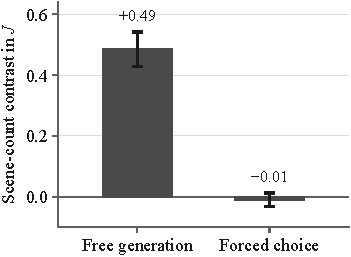
\includegraphics{fig_forced.pdf}\par}
\caption{The scene-count contrast in free generation, where the model selects which objects to
name, and as a forced-choice probe, where the question supplies the object; $95\%$ intervals.}
\label{fig:forced}
\end{minipage}\hfill
\begin{minipage}[t]{0.52\textwidth}
\vspace{0pt}
\makeatletter\def\@captype{table}\makeatother
\caption{Every probe fails all three off-ceiling conditions fixed in advance (pooled over arms):
C1~$\rateF \in [0.20, 0.80]$, C2~$\rateT \le 0.90$, C3~yes-rate~$\in [0.15, 0.85]$. Image-only:
``answer only from the image''; mixed: adds ``some are, some are not''. Closed-set rows:
calibration, $n = 478$.}
\label{tab:unsatceiling}
\centering
\footnotesize
\setlength{\tabcolsep}{4pt}
\begin{tabular}{@{}lrrr@{}}
\toprule
probe & \rateT{} & \rateF{} & yes-rate \\
\midrule
published probe & $0.9732$ & $0.8796$ & $0.8949$ \\
published probe, re-run here & $0.9739$ & $0.8791$ & $0.8945$ \\
image-only prompt & $0.9711$ & $0.8622$ & $0.8799$ \\
two-alternative choice & $0.9437$ & $0.9347$ & $0.9362$ \\
closed candidate set & $1.0000$ & $1.0000$ & $1.0000$ \\
closed candidate set, mixed & $1.0000$ & $0.9949$ & $0.9958$ \\
\bottomrule
\end{tabular}
\end{minipage}
\end{figure}

\paragraph{The objection.} The registered forced-choice probe moves the scene-count contrast by
$+0.4859$ under free generation and by $-0.0095$ \civ{-0.0314}{+0.0124} under forced choice on
identical units (Figure~\ref{fig:forced}). But the published forced-choice probe is saturated: its
false-positive rate rises from $0.022$ with no prefix to $0.8714$ and $0.8835$ under the one- and
five-scene prefixes, and it fails every off-ceiling condition fixed in advance
(Table~\ref{tab:unsatceiling}). Its null could mean that forced choice removes the selection step
carrying the effect, or that the probe would return a null for anything.

\paragraph{Changing the probe does not de-saturate it.}\label{app:unsat-gate} We pre-registered four
candidate probes, each read in one forward pass as a probability $p_{\mathrm{yes}}$ over two fixed
answer-token groups and thresholded for the binary answer. All four stay at ceiling, the closed
candidate set with never-mentioned distractors hardest, at a yes-rate of $1.0000$. A post-hoc
diagnostic on the two-alternative variant shows why: it chooses the unit object at $0.9362$ when the
prefix named it and $0.4990$ when it did not, so the binary format measures prefix membership. The
registered outcome is ``still saturated'', which returns no verdict.

\paragraph{The graded readout of the published probe.} Registered to be reported in every branch, it
gives $+0.0008$ \civ{-0.0142}{+0.0166}, width $0.0309$ against $0.0425$ for the binary answer, and
it is not pinned: between $61\%$ and $74\%$ of each arm's units have $p_{\mathrm{yes}}$ inside
$(0.05, 0.95)$. That evidence is post-hoc, because the registered ceiling gate was defined on the
binary rate and triggered.

\paragraph{Scoring objects the prefix never names.}\label{app:unsat-scope} A second pre-registered
analysis scores distractors, objects the prefix never mentions, with the two-alternative probe;
prefix membership is constant across them and cannot pin the readout. The registration names the
binary readout as primary, gated by the conditions of Table~\ref{tab:unsatceiling}, and the graded
readout as co-primary, gated on the graded quantity itself (interior fraction at least $0.50$,
$p > 0.99$ fraction at most $0.10$). Both gates were fixed before any five-scene row existed (the
earlier run had produced one-scene rows only), and a failure of one does not block the other. Free
generation on these units moves by $+0.3655$ \civ{+0.2987}{+0.4303}, so there is an effect to find.
The binary primary missed its ceiling gate ($\rateT = 0.9041$ against a ceiling of $0.90$), so the
registered outcome is ``distractor probe saturated'', which is not a verdict. The graded co-primary passed
its own gate: the forced-choice register moves by $-0.0057$ \civ{-0.0153}{+0.0036}, or
$-0.006 \pm 0.010$ once widened in quadrature by run-to-run replay noise, and the readout is live on
the same units and scale, registering ground-truth presence at $+0.2981$ ($0.7966$ against $0.4985$).
The registration reports the two readouts independently, but its pre-committed reading accepts a null
verdict only if the binary gates pass. They did not, so the graded null is supporting evidence and not
a registered confirmation.

\paragraph{Corrections.} The first scoring run reported ``distractor probe saturated'' as the headline
cell. A later change to the headline selector, reasoning from the clause that the two readouts are
gated independently, reported the co-primary's ``distractor null confirmed'' instead; every
number is identical between the two runs, and both result files are kept. That change conflicts with
the registration's pre-committed acceptance rule for a null, which requires the binary gates to pass.
We follow the stricter clause: the registered outcome is ``distractor probe saturated''. Separately, a replay gate shown to reject a perfect re-run of the earlier probe was
replaced before endpoint generation by one requiring exact agreement away from the decision boundary.

\paragraph{Scope.} Both graded analyses are consistent with a forced-choice null that does not
depend on prefix-membership pinning, since this one scores units where pinning cannot operate.
Neither is a registered confirmation: the earlier graded readout is post hoc, and this one is excluded
from confirmation by its registration's own acceptance rule. No off-ceiling binary probe was
obtained.


\section{The Ablation Ladder}
\label{app:ladder}

Section~\ref{sec:twofactors} reports that the answer to ``does the rise need the image?'' depends on the
ablation. This appendix gives the ten ablations, how severe each one is, and what each returns.

\paragraph{Construction.} Every ablation is applied to the canonical $336 \times 336$ image the
processor produces, so geometry is identical across arms; a gate asserts $32/32$ byte-identical
geometry against the unablated path. \texttt{noise}$k$ adds uniform pixel noise of amplitude $k$;
\texttt{blur}$k$ applies a Gaussian blur of radius $k$; \texttt{lowres16} downsamples to $16
\times 16$ and back; \texttt{shuffle24} permutes $24 \times 24$ patches; \texttt{grey} and
\texttt{black} replace the image with a uniform field; \texttt{mismatch} substitutes a different
real COCO image under a derangement (seed $20260919$, asserted bijective and self-pair-free).
Prefix token ids are bit-identical across all arms. $n = 3000$ cells per rung on the prefix
endpoint ($1500$ per condition), $500$ images on CHAIR.

\paragraph{Severity.} We define severity as $1 - \cos$ between the mean-pooled image features the
model's own vision pathway produces for the clean and the ablated image. It is a property of the
ablation, measured before any endpoint is read. It measures \emph{displacement in feature space},
not destruction of task-relevant content, and we have not validated it against a downstream task:
two real scenes share much of their mean-pooled structure, while a uniform field is out of
distribution for the encoder, so the substitution can displace features less than a blank while
destroying far more of what the endpoint scores. Claims below are therefore about displacement, and
the substantive point is the four named counterexamples rather than the ordering as a whole.

\paragraph{Reading.} The seven graded pixel ablations pool to $-0.006$ \civ{-0.037}{+0.025}; the
substitution returns $+0.160$ \civ{+0.105}{+0.213}, and the paired difference against grey is
$+0.176$ \civ{+0.119}{+0.230}. As blind-to-sighted ratios the same contrast is $1.033$
\civ{0.921}{1.160} under grey against $0.671$ \civ{0.573}{0.774} under the substitution; these are
the two figures the main text compares. Over the nine pixel ablations severity and $\dSight$ have a rank
correlation of $+0.10$; with $n = 9$ that is uninformative and we draw no conclusion from it. What
does the work is the four named counterexamples --- \texttt{lowres16}, \texttt{black}, \texttt{grey}
and \texttt{blur16} --- each displacing the image further than the substitution and each returning
an interval containing zero. The contribution sits in the hit rate ($\Delta H = +0.149$
\civ{+0.097}{+0.201} against $\Delta F = -0.010$ \civ{-0.034}{+0.013}): with the true image $H$
rises $0.676 \to 0.780$ across the contrast, with a substituted one it \emph{falls} $0.644 \to
0.599$. Grey hides this by collapsing the one-scene $H$ to $0.468$, preserving the difference while
destroying the level. Cross-condition length matching gives $+0.138$ \civ{+0.096}{+0.181}.

\paragraph{The substitution arm is not degenerate.} Pooled over both conditions its median
continuation is $384$ tokens against grey's $60$, its empty rate $0.017$ against $0.025$, its
$\le 3$-token rate $0.082$ against $0.124$, and it produces $2848$ distinct continuations of $3000$
against grey's $2693$. It is healthier than the arm it is compared with.

\paragraph{Registration and one amendment that mattered.} The ladder was pre-registered before any
rung was generated, with three dated amendments. Amendment~3 replaced a \emph{comparative} collapse
screen (``no more degenerate than the reference arms'') with absolute thresholds, because in the
five-scene condition both reference arms sit at the $384$-token generation budget, so a bar of
$\min(\text{sighted},\text{grey})$ equals the ceiling and flags every rung that terminates
naturally; the diversity ratios fall mechanically with length and have the same fault. The
amendment was written before any ladder verdict was read and it changed exactly one verdict --- the
substitution arm, from ``confounded by collapse'' to ``image contributes'', on an
$8$-gram ratio of $0.567$ against $0.575$. Under the original screen, the substitution result
would have been discarded by a screen whose form was wrong.

\paragraph{Positive controls.} The scorer reproduces the published $\dPrim = +0.4859$, $\dBlind =
+0.5019$ and $\dSight = -0.0160$ to $3 \times 10^{-5}$, and a re-generation of the grey arm is
$3000/3000$ token-identical to the published one with $\dSight$ reproducing to $0.000000$.

\paragraph{On CHAIR.} Under grey, and equally under flat black, the model names none of the $80$
categories in any of $500$ captions, so $\mathrm{CHAIR}_i$ is $0/0$. Every graded degradation leaves
the denominator non-empty: $500$, $500$, $498$, $489$, $378$, $405$, $450$ and $500$ captions of
$500$ retain a category mention under \texttt{noise16/32/64}, \texttt{blur4}, \texttt{blur16},
\texttt{lowres16}, \texttt{shuffle24} and \texttt{mismatch} respectively. Against a sighted PAI gain
of $+5.56$ in $\mathrm{CHAIR}_i$ (this experiment's resample gives \civ{+3.88}{+7.18}, the PAI experiment's
\civ{+3.88}{+7.10}), the image-attributable part is $+5.16$
\civ{+2.89}{+7.42} under substitution. Under \texttt{blur16} it is $+8.70$ \civ{+2.55}{+14.96},
more than the whole gain, so PAI raises $\mathrm{CHAIR}_i$ on the $378$ blurred captions that keep a
mention; with that denominator shrinking, we do not use the blur arm as evidence. The
three noise rungs retain the gain but fail the registered severity floor and are not quoted as
evidence. On this prompt-only endpoint the substitution arm is algebraically the registered
permuted-ground-truth secondary evaluated at a single derangement; the secondary averages twenty.

\paragraph{Not done.} \textsc{LLaVA-OV-0.5B} was not run on the ladder: its processor uses AnyRes
multi-crop, so the canonical geometry the geometry gate licenses does not transfer and the gate
would need redesigning first.


\section{POPE with a Blind Arm}
\label{app:pope}

\paragraph{Data.} Official POPE files from \texttt{RUCAIBox/POPE}, all three MS-COCO splits
(\texttt{random}, \texttt{popular}, \texttt{adversarial}), $3000$ questions each for $9000$ total
over $500$ distinct images, exactly $1500$ yes and $1500$ no per split, with per-file sha256
re-asserted at every load. Because the splits are balanced, $H$ is the reported recall and
$F = H + 1 - 2\,\mathrm{acc}$ exactly; the scorer asserts this identity on every cell and it holds
to $2.2\times10^{-16}$ across $48$ cells.

\paragraph{A snapshot trap.} \textsc{LLaVA-1.5}'s own evaluation documentation points at a
different POPE snapshot whose \texttt{random} split has $2910$ questions at $1500$ yes / $1410$ no.
An all-``yes'' responder scores $51.55$ there against $50.00$ on the balanced file, so the balanced
identity above does not hold for numbers computed on that snapshot. We use the current balanced
files throughout.

\paragraph{Arms.} \texttt{vanilla} ($\alpha = 0$, $\gamma = 1$, kernel- and loop-matched rather than
a separate code path), \texttt{pai\_full} ($\alpha = 0.5$, $\gamma = 1.1$; the released
\texttt{--use-attn --use-cfg}), \texttt{pai\_attn} ($\alpha = 0.5$, $\gamma = 1.0$; attention only,
amplifying the prefill row), and \texttt{pai\_both}, a constructed configuration that is not a
released one and is labelled as such wherever it appears. All arms are greedy; no contrast compares
across decoding modes. Ablations: sighted, grey, and a mismatched real image, plus a severity ladder
(\texttt{noise25/50/100}, \texttt{blur4}, \texttt{blur16}, \texttt{lowres}, \texttt{pshuffle}).

\paragraph{Result.} On \texttt{pai\_attn} --- the configuration that reproduces PAI's published POPE
number, $+1.10$ accuracy points against their $+1.06$ --- the gain is \emph{partly} attributable to
the image, at the registered label ``partial'' defined below:
$\Delta_{\text{sighted}}(J) = +0.0220$ \civ{+0.0107}{+0.0336}, $\Delta_{\text{ablated}}(J) = +0.0013$
\civ{-0.0102}{+0.0124}, and $\Delta_{\text{image}}(J) = +0.0207$ \civ{+0.0042}{+0.0371}; in accuracy
$+1.033$ \civ{+0.21}{+1.86}. $B = 4000$, paired, clustered on the $500$ images. The registered label
is ``partial'' rather than ``image-attributable'', because the lower bound $+0.0042$ falls
below the pre-registered half-gain line of $0.0110$, so the rule cannot certify that more than half
the gain is image-attributable. \texttt{pai\_both} agrees ($+0.0238$ \civ{+0.0078}{+0.0398}).

\paragraph{The released default measures nothing.} \texttt{pai\_full} gives
$\Delta_{\text{image}} = +0.000$. Its attention stage is guarded so that the conditional prefill pass
is never amplified, and on POPE the answer is the first generated token; \texttt{pai\_both} and
\texttt{pai\_full} differ only in whether the prefill last row is touched, and that difference is
worth $+1.112$ accuracy points against $+0.056$ for the decoding-distribution stage. The whole
published gain lives in one attention row.

\paragraph{The grey arm returns no data.} Under grey the model answers ``no'' to all $9000$
questions, fluently and correctly --- a grey field contains none of the queried objects --- so
$H = F = 0$ by construction, $\Delta_{\text{ablated}}$ is mechanically zero, and an unguarded reading
would have returned ``image-attributable'' while measuring nothing. The registration forbade
that reading in advance: the arm is ``blind arm degenerate'' and $\Delta_{\text{image}}$ is
undefined, not null. The severity ladder shows the same dissociation as Appendix~\ref{app:ladder}:
\texttt{blur16} retains $J = +0.19$ while a sharp photograph of another scene retains $+0.04$, and
\texttt{pshuffle} dissociates the rates ($H$ $0.883 \to 0.857$ while $F$ $0.184 \to 0.330$).

\paragraph{Gates and controls.} Fifteen blocking gates passed before any endpoint was read,
including per-item token identity across arms with zero padding, exactly $576$ image tokens per row,
copy-drift token-identity against the original kernel, $0/4$ decode mismatches against Hugging
Face \texttt{generate}, post-softmax mass on strictly-future keys exactly $0.0$, and determinism
$0/288$. Positive control: our \texttt{vanilla} sighted arm scores $84.91$ accuracy against PAI's
published $84.76$.

\paragraph{PAI's own published table, recoded.} On POPE's balanced splits the two coordinate systems
interconvert exactly: $\mathrm{acc} = (H + 1 - F)/2$ and $\mathrm{F1} = 2H/(1 + H + F)$, so
$F = H + 1 - 2\,\mathrm{acc}$ and $H = \mathrm{F1}\,(1 - \mathrm{acc})/(1 - \mathrm{F1})$. PAI's
Table~2 \citep{pai} reports accuracy and F1 for \textsc{LLaVA-1.5} under single-turn greedy decoding;
recoded, it gives Table~\ref{tab:paipub}. The recoding is derived, not measured: it carries no
interval, inherits the equal-variance assumption behind $d'$ and $c$, and is approximate because F1,
unlike accuracy, does not average exactly over the three splits. It is a cross-check on
Table~\ref{tab:pai}, which shows the same ordering, $\Delta c$ well above $\Delta d'$.

\begin{table}[h]
\caption{PAI's published POPE result \citep[Table~2]{pai}, recoded into rates and signal-detection
coordinates.}
\label{tab:paipub}
\begin{center}
\small
\begin{tabular}{lrrrrrrr}
\toprule
Arm & Acc & F1 & $H$ & $F$ & $J$ & $d'$ & $c$ \\
\midrule
Vanilla & $84.76$ & $85.51$ & $0.899$ & $0.204$ & $+0.695$ & $+2.105$ & $-0.226$ \\
PAI     & $85.82$ & $85.97$ & $0.869$ & $0.153$ & $+0.716$ & $+2.147$ & $-0.048$ \\
\midrule
Change  & $+1.06$ & $+0.46$ & $-0.031$ & $-0.052$ & $+0.021$ & $+0.042$ & $+0.178$ \\
\bottomrule
\end{tabular}
\end{center}
\end{table}

\paragraph{Registration.} Pre-registered before the first generation job, with two dated amendments
(the mismatched-image co-primary, and a frame-equivalence fix after a rounding discrepancy was found
and corrected from $2.221$ to $0.030$ maximum absolute pixel difference).


\section{\textsc{Qwen3-VL-8B}}
\label{app:qwen3}

\paragraph{Checkpoint and environment.} \texttt{Qwen/Qwen3-VL-8B-Instruct} \citep{qwen3vl}, revision
\texttt{0c351dd0}, $8{,}767{,}123{,}696$ parameters, bfloat16, one RTX 4090. This experiment ran under a
different interpreter from the other architectures (\texttt{torch} 2.11.0, same
\texttt{transformers} 5.14.1) because the base interpreter has neither PIL nor torchvision, so no
vision-language processor loads in it.

\paragraph{Template and cut.} The prompt template is the processor's own
\texttt{apply\_chat\_template} output, frozen to disk and byte-compared by every later stage. It
carries \emph{no} system turn, unlike \textsc{Qwen2.5-VL}'s. The realised census cut is $0.205$.
Free-running continuations hit the $256$-token cap on $99.2\%$ of images, so the per-cell budget is
near-constant rather than image-keyed; this cut is therefore not comparable to the $0.230$ and
$0.460$ of the other architectures.

\paragraph{Harness gate, calibrated against our own lead model.} Before any endpoint was generated,
six gates ran. The decisive one exploits greedy determinism: cut the model's own caption at the
census cut, splice it back as an assistant-turn prefill, and require it to re-emit the remainder. A
broken template cannot pass this; a merely terse model can. \textsc{Qwen3-VL-8B} scores a median
$16$-gram agreement of $1.000$, mean $0.958$, with $92\%$ of rows above threshold. The identical test
run on \textsc{LLaVA-1.5-7B} in the same job scores $1.000$, $0.945$ and $92\%$. The bar therefore
comes from this paper's own lead model rather than from an invented threshold, and the verdict was
``run endpoint''; the endpoint arms were held and released only on that verdict.

\paragraph{Result.} $\dPrim = +0.5828$ \civ{+0.5337}{+0.6342}, $\dBlind = +0.5231$
\civ{+0.4708}{+0.5764}, $\dSight = +0.0598$ \civ{+0.0235}{+0.0963}, $n = 1500$ cells per arm,
$B = 4000$ clustered on the image with one joint resample across all four arms. The interval
excludes zero, so on this architecture part of the rise does need the image --- but it lies entirely
inside the $\pm 0.10$ reference band, so about $90\%$ of the rise still survives blinding. The
contribution is confined to the five-scene condition ($+0.0612$ \civ{+0.0392}{+0.0841}) and absent in
the one-scene condition ($+0.0014$ \civ{-0.0262}{+0.0285}).

\paragraph{Not the \textsc{Qwen2.5-VL} failure.} The degeneracy screen passes on all four arms:
median continuation $384$ tokens in every arm, empty rates $0.000$ to $0.003$, $\le 3$-token rates
approximately zero. Supporting contrasts: length-matched $\dPrim = +0.576$ and $\dBlind = +0.511$;
object-matched $+0.565$; empty-removed $+0.584$; alternate seed $+0.583$.

\paragraph{A screen we now know is insufficient.} Our degeneracy screens test length and short-output
rate, not repetition. Measured after the fact, $90\%$ and $83\%$ of this model's cells fall below a
$0.5$ distinct-$8$-gram ratio --- but so do $67.5\%$ of the lead model's five-scene cells, so looping
is a property of the design rather than of this architecture. The sighted and blind arms nonetheless
loop at different rates ($0.827$ against $0.911$) in exactly the condition carrying $\dSight$, and no
looping-matched contrast was run. \textsc{Qwen2.5-VL}'s apparently clean ratio of $1.0000$ is an
artefact: four-token continuations contain no $8$-gram.

\paragraph{A mismatched-image arm (post hoc).} After the registered experiment, we ran the substitution of
Appendix~\ref{app:ladder} on this model: the same $1{,}500$ cells and prefixes, each image replaced by
another of the $500$ under the derangement with seed $20260919$ (asserted bijective and self-pair-free,
$3{,}000$ rows). Every hard gate of the registered scorer passed; its grey-flag gate, which requires the
ablated arm to be grey, was inverted to require that no arm is grey and that every substituted row was
generated from a different image. The scorer's positive controls reproduced both reference families
($+0.48587$ against $+0.4859$; $+0.15981$ against $+0.1598$), and the sighted contrast reproduces
$+0.583$. The substituted contrast is $+0.518$ \civ{+0.464}{+0.571}, so $\dSight = +0.065$
\civ{+0.031}{+0.100} (ratio $0.89$), against $+0.060$ \civ{+0.023}{+0.096} (ratio $0.90$) under grey.
The two ablations agree on this model. Its one-scene $J$ is $+0.049$ sighted and $+0.050$ substituted
($H$ $0.83$, $F$ $0.78$): the model repeats most passage objects in the one-scene condition, with
or without the correct image, so there is no one-scene level for a blank to destroy, and the image's
contribution sits entirely in the five-scene condition ($+0.065$ \civ{+0.042}{+0.087}). The regime
factor cannot be tested here: $94\%$ of continuations reach the budget and only $14$ cells are
untruncated.

\paragraph{Registration.} Pre-registered before the checkpoint existed locally, fixing the gate
thresholds, the census rule, the arms, the estimand, and the text to be published for every outcome
including the two adverse ones. The estimator was validated before any \textsc{Qwen3-VL} row existed
by reproducing two published families from their frozen rows: $+0.48587$ against a published
$+0.4859$, and $+0.15981$ against $+0.1598$.


\section{Both Ablations on the 3{,}500-Image Sample}
\label{app:regimeblind}

Appendix~\ref{app:regime} controls the generation regime on the sighted arms by restricting to
cells where neither condition reaches the $384$-token budget, which drops the contrast from
$+0.472$ on all $10{,}500$ cells of the $3{,}500$-image sample to $+0.346$. That control had no
ablated arm. This appendix supplies two, the grey field and the mismatched real image of
Appendix~\ref{app:ladder}, each run on all $10{,}500$ cells, so every cell of the $2 \times 2$ in
Figure~\ref{fig:lead}(b) is computed on one population. The whole extension is post hoc.

\paragraph{Construction.} Each ablated generator is the sighted generator with one line changed. For
grey, the target image is replaced by a flat mid-grey field of its own pixel dimensions, through the
same mirrored code path used for the published blind arms. For the substitution, each image is
replaced by another image of the same block under a derangement (seed $20260919$, asserted bijective
and self-pair-free, $875$ images per block). Prefix token ids, cell construction, sort order and
batch size are untouched. Gates ran before any row was kept, on all four blocks: for grey, a mirror
gate requiring the blind code path with the substitution \emph{off} to reproduce the sighted
generator token-for-token (\textbf{32/32} identical in every block); for both, a prefix-drift gate
against the published cells (\textbf{0} of $3{,}000$ published prefixes drift) and a census gate on
the cell md5s (\textbf{0} of $5{,}250$ per block). Each arm is $21{,}000$ rows. The derangement is
reconstructed at scoring time and checked against the text: under the substitution, $54.6\%$ of the
objects a continuation names are in the substitute image's ground truth and $18.7\%$ in the
target's, against $19.0\%$ and $54.1\%$ sighted.

\paragraph{Cell sets and positive controls.} ``All cells'' is every cell with both conditions in all
three arms ($10{,}500$ cells, $3{,}500$ images). ``Untruncated'' applies the \emph{registered} regime rule
to the sighted arms only --- both sighted continuations below the budget --- giving $2{,}089$ cells on
$1{,}649$ images. On that set the sighted contrast is $+0.3460$, reproducing the registered value in
Table~\ref{tab:regime} to four decimals, and the two ablated estimates reproduce their first scoring
runs to four decimals. The rule does not constrain the ablated arms: inside the untruncated cells grey
continuations still reach the budget in $2\%$ (one scene) and $27\%$ (five scenes) of cases, and
substituted ones in $11\%$ and $27\%$. On all cells the three arms reach it at similar rates (sighted
$48\%$ and $69\%$, substituted $47\%$ and $69\%$), except grey's one-scene arm ($25\%$).

\begin{table}[h]
\caption{The one-to-five-scene contrast under each ablation on the $3{,}500$-image sample. The one- and
five-scene columns give $J = H - F$ in each condition. Intervals are $B = 4000$ bootstrap replicates clustered on the
image. Ratio is the ablated contrast over the sighted one; its intervals are percentile intervals of the
replicate ratios.}
\label{tab:regimeblind}
\begin{center}
\footnotesize
\setlength{\tabcolsep}{2.4pt}
\begin{tabular}{llrrrll}
\toprule
Cells & Arm & One scene & Five scenes & Contrast & $\dSight$ & Ratio \\
\midrule
All      & Sighted          & $+0.176$ & $+0.647$ & $+0.472$ & --- & --- \\
($10{,}500$) & Grey field   & $-0.028$ & $+0.447$ & $+0.475$ & $-0.003$ \civ{-0.025}{+0.019} & $1.01$ \civ{0.96}{1.05} \\
         & Mismatched & $+0.099$ & $+0.418$ & $+0.319$ & $+0.153$ \civ{+0.132}{+0.175} & $0.68$ \civ{0.64}{0.72} \\
\midrule
Untruncated & Sighted          & $+0.105$ & $+0.451$ & $+0.346$ & --- & --- \\
($2{,}089$) & Grey field    & $-0.069$ & $+0.177$ & $+0.246$ & $+0.100$ \civ{+0.041}{+0.163} & $0.71$ \civ{0.56}{0.87} \\
         & Mismatched & $+0.057$ & $+0.221$ & $+0.164$ & $\mathbf{+0.182}$ \civ{+0.122}{+0.245} & $0.47$ \civ{0.33}{0.62} \\
\bottomrule
\end{tabular}
\end{center}
\end{table}

\paragraph{Result.} On all cells the $3{,}500$-image sample reproduces both registered-sample
answers --- grey $1.01$ against $1.03$, substitution $0.68$ against $0.67$ --- and $3{,}000$ of its
images played no part in either. Restricting to untruncated cells moves both
(Table~\ref{tab:regimeblind}). Under grey the untruncated one-scene level falls below zero ($-0.069$
against $+0.105$ sighted), the level collapse the blank produces on the registered sample. The
substitution keeps the one-scene level near the sighted one ($+0.057$), and it is the five-scene gain
that shrinks.

\paragraph{The substitute image is not information-free.} A real image contains common objects, and
the passage's present objects are enriched for them: $46$--$48\%$ of present units on all cells
($41$--$42\%$ untruncated) name an object that the substitute image also contains, against $10$--$12\%$
of absent units. For those units the substituted arm still has visual evidence. Excluding them from
every arm raises $\dSight$ to $+0.241$ \civ{+0.211}{+0.270} on all cells (ratio $0.46$
\civ{0.40}{0.52}) and to $+0.266$ \civ{+0.192}{+0.342} on untruncated cells (ratio $0.22$
\civ{0.02}{0.39}). The overlap therefore biases the substitution towards finding no image
contribution, and the estimates in Table~\ref{tab:regimeblind} are conservative. The exclusion
changes the population scored, so we report it as evidence on the direction of the bias, not as a
replacement estimate.

\paragraph{What this does not settle.} The substitution uses one derangement. The untruncated cells are
those that terminate naturally under \emph{both} sighted conditions, a population that is easier to
caption than the sample as a whole, and the rule does not force the ablated arms to terminate.


\end{document}
